%% uctest.tex 11/3/94
%% Copyright (C) 1988-2004 Daniel Gildea, BBF, Ethan Munson.
%
% This work may be distributed and/or modified under the
% conditions of the LaTeX Project Public License, either version 1.3
% of this license or (at your option) any later version.
% and version 1.3 or later is part of all distributions of LaTeX
% version 2003/12/01 or later.
%
% This work has the LPPL maintenance status "maintained".
% 
% The Current Maintainer of this work is Daniel Gildea.
%
% 2007/08/01
% LaTeX Package "ucr" is modified from LaTeX package "ucthesis."
% This modification is therefore under to the conditions of 
% the LaTeX Project Public License.
% Its formality is suitable for the dissertation of Universty of
% California, Riverside.
% This test document is for the convenience of all students of
% Universty of California, Riverside.
% Contact Charles Yang at chcyang@yahoo.com if you like.
% Charles Yang has nothing to do with the original author's sarcasm.
%
% \documentclass[11pt]{ucthesis}
% \documentclass[11pt]{ucr}
\documentclass[oneside, final]{ucr}

\usepackage{booktabs}
\usepackage{tabularx}
\usepackage{graphicx}%
\usepackage{multirow}%
\usepackage{amssymb}
\usepackage{algorithm}%
\usepackage{algorithmicx}%
\usepackage{algpseudocode}%
\usepackage{listings}%
\usepackage[toc,page]{appendix}
\usepackage[all]{nowidow}
%\usepackage{refcheck}

%% For algorithms...
\algnewcommand\algorithmicforeach{\textbf{for each}}
\algdef{S}[FOR]{ForEach}[1]{\algorithmicforeach\ #1\ \algorithmicdo}
\algnewcommand\algorithmicswitch{\textbf{switch}}
\algnewcommand\algorithmiccase{\textbf{case}}
\algdef{SE}[SWITCH]{Switch}{EndSwitch}[1]{\algorithmicswitch\ #1\ \algorithmicdo}{\algorithmicend\ \algorithmicswitch}
\algdef{SE}[CASE]{Case}{EndCase}[1]{\algorithmiccase\ #1}{\algorithmicend\ \algorithmiccase}
\algtext*{EndSwitch}
\algtext*{EndCase}
%%%%

\setlength{\footskip}{0.55in}

\begin{document}

% Declarations for Front Matter

\title{Scaling Spatial Overlay Operations and Flock Pattern Discovery}
\author{Andres Oswaldo Calderon Romero}
\degreemonth{December}
\degreeyear{2024}
\degree{Doctor of Philosophy}
\chair{Dr. Vassilis Tsotras}
\othermembers{
Dr. Amr Magdy\\
Dr. Petko Bakalov\\
Dr. Ahmed Eldawy\\
Dr. Vagelis Hristidis\\
}
\numberofmembers{5}
\field{Computer Science}
\campus{Riverside}

\hypersetup{pageanchor=false}
\maketitle
\hypersetup{pageanchor=true}
\copyrightpage{}
\approvalpage{}

\degreesemester{Fall}

\begin{frontmatter}

\begin{acknowledgements}

First and foremost, I would like to express my heartfelt gratitude to my advisor, Prof. Vassilis Tsotras. His guidance, patience, and insightful feedback have been invaluable throughout this journey. I feel privileged and honored to have worked under his supervision and am deeply indebted to him. I aspire to one day become as exceptional an advisor as he has been to me. Thank you.

In addition, I would like to extend my sincere gratitude to Petko Bakalov, Marcos Vieira, Laila Abdelhafeez, and Amr Magdy for their invaluable support in the work I present here. I am deeply grateful for your time, assistance, and encouragement.

And to my love, Nancy – you have been there for me whenever I needed you, offering boundless support and encouragement. Through countless moments when I felt like giving up, you continued to believe in me. Your presence has been extraordinary and essential to my journey. I love you and our family.

\end{acknowledgements}


\begin{dedication}
\null\vfil
{\large
\begin{center}
\textit{To Nancy, my beloved wife, and to our flock.}
\end{center}}
\vfil\null
\end{dedication}


\begin{abstract}
This thesis proposes scalable solutions to two significant spatial problems: computing overlay operations and discovering flock patterns. Overlay operations are typically computed among polygon layers using spatial data structures designed for complex geometric relationships. One such structure is the Doubly Connected Edge List (DCEL), an edge-list format widely used in spatial applications for performing planar topological computations. The overlay operation, which combines the DCELs of two input layers, enables efficient spatial queries such as intersection, union, and difference between layers. However, existing sequential methods for computing overlays struggle to scale and often fail to process large datasets, such as the US Census tracts. In this thesis, we present a distributed, scalable approach for computing the overlay operation and its associated queries. We address the challenges inherent in distributing the overlay computation and introduce several optimizations that enhance performance, making these computations feasible for large-scale spatial datasets.

The second part of this thesis extends upon the above proposed approach by introducing a novel spatial partitioner based on the kd-tree spatial index. This partitioner optimizes DCEL partitioning and overlay operations by leveraging data distributions, resulting in significantly improved performance and more efficient space utilization. Additionally, we adapt the optimization techniques developed for DCEL overlay operations to address a new problem: the polygonization of dangling edges, cut edges, and polygons.

The final part of this thesis presents a scalable technique for detecting moving flock patterns in large trajectory databases. A flock pattern represents a group of entities moving closely together within a defined spatial radius over a specified time interval. Traditional sequential algorithms, though effective, struggle with high computational costs on large, dense datasets. This thesis proposes a distributed framework that leverages spatial partitioning and parallel processing to accelerate flock detection. By addressing challenges in spatial and temporal joins across large datasets, introducing partition-based parallelism, and implementing strategies to manage flock patterns spanning multiple partitions, this approach significantly reduces processing time. Experimental evaluations on synthetic datasets demonstrate substantial improvements in scalability and efficiency over conventional methods.
\end{abstract}


\tableofcontents
\listoffigures
\listoftables
\end{frontmatter}

%\msp
\section{Introduction} %\label{sec:extenstion_introduction}

This chapter extends the previous work in \cite{calderon_scalable_2023}. The main new contributions are summarized as follows. First, we introduce a new spatial partitioner, based on the kd-tree partitioning strategy, for constructing overlay  DCELs (section \ref{sec:pstrategies}). Since it better utilizes the data distributions in optimizing DCEL partitions, it leads to noticeably improved performance. The new partitioning strategy contrasts with the original strategy that employed space-partitioning techniques based on quadtrees. 

Second, we extend the overlay DCEL approach to accept scattered and noisy line segments as input, rather than being restricted to clean polygon data. This enhancement builds on the scalable polygonization methods presented in \cite{abdelhafeez_ddcel_2023}, enabling the overlay of real-world datasets composed of vast sets of line segments —datasets that existing techniques are unable to process effectively.

For instance, Figure \ref{fig:extension_dcel_example} illustrates the fundamental components of a DCEL. Additionally, we identify two types of special half-edges. \textit{Dangles} are half-edges with one or both endpoints not incident on another half-edge endpoint; both half-edge $\overrightarrow{fj}$ and its twin are considered dangle edges. \textit{Cut-edges} are half-edges connected at both ends that do not form part of any polygon. The half-edge $\overrightarrow{dg}$ and its twin are classified as cut-edges.

\begin{figure}
    \centering
    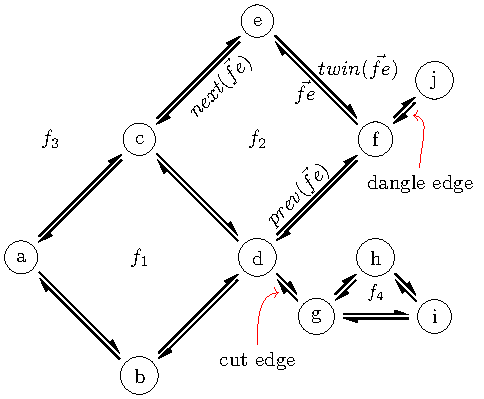
\includegraphics[width=0.6\linewidth]{chapterExtension/dcel_example2}
    \caption{Components of the DCEL structure with dangle and cut edges.}\label{fig:extension_dcel_example}
\end{figure}

The remainder of this chapter is organized as follows. Section \ref{sec:extension_methods} details the implementation of the new kd-tree partitioner and describes the polygon extraction process for adapting line segment inputs, which extends the overlay method to support dangle and cut edges. In Section \ref{sec:extension_experiments}, we present additional experiments to quantify the benefits of the kd-tree-based strategy and assess the performance of the proposed polygonization on datasets with large volumes of line segments.

\chapter{Scalable Overlay Operations over DCEL Polygon Layers}

\section{Introduction}

The use of spatial data structures is ubiquitous in many spatial applications, ranging from spatial databases to computational geometry, robotics, and geographic information systems \cite{samet_design_1990}. Spatial data structures have been used to improve the efficiency of various spatial queries, spatial joins, nearest neighbors, Voronoi diagrams, and robot motion planning. Examples include grids \cite{nievergelt_grid_1984}, R-trees \cite{guttman_r-trees_1984, beckmann_r-tree_1990}, and quadtrees \cite{finkel_quadtrees_1974}.  \textit{Edge-list} structures are also typically utilized in applications as topological computations in computational geometry \cite{berg_computational_2008}.

The most commonly used data structure in the edge-list family is the \textit{Doubly Connected Edge List (DCEL)}. A DCEL \cite{muller_finding_1978, preparata_computational_1985} is a data structure that collects topological information for the edges, vertices, and faces contained by a surface in the plane. The DCEL and its components represent a planar subdivision of that surface. In a DCEL, the faces (polygons) represent non-overlapping areas of the subdivision; the edges are boundaries that divide adjacent faces; and the vertices are the point endings between adjacent edges (see Figure \ref{fig:dcel_example}).  In addition to providing geometric and topological information, a DCEL can be enhanced to provide further information. For instance, a DCEL storing a thematic map for vegetation can also store the type and height of the trees around the area \cite{berg_computational_2008}.

\begin{figure}
    \centering
    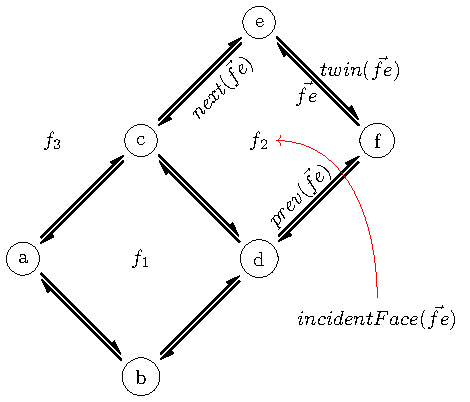
\includegraphics[width=0.6\linewidth]{chapterSDCEL/dcel_example}
    \caption{Components of the DCEL structure.}\label{fig:dcel_example}
\end{figure}

The DCEL data structure has been used in various applications. For instance, the use of connected edge lists is cardinal to support polygon triangulations and their applications in surveillance (the Art Gallery Problem \cite{chvatal_combinatorial_1975, orourke_art_1987}) and robot motion planning (\cite{berg_computational_2008, chew_convex_1993}). DCELs are also used to perform polygon unions (for example, on printed circuit boards to support the simplification of connected components in an efficient manner \cite{fogel_cgal_2012}) as well as the computation of silhouettes from polyhedra \cite{fogel_cgal_2012, berberich_arrangements_2010} (applied frequently in computer vision and 3D graphics modeling \cite{boguslawski_modelling_2011}).

Edge-list data structures have also been utilized to create thematic \textit{overlay maps}. In this problem, the input contains the DCELs of two polygonal layers, each capturing geospatial information and attribute data for different phenomena, and the output is the DCEL of an overlay structure that combines the two layers into one. In many application areas, such as ecology, economics, and climate change, it is important to be able to join the input layers and match their attributes in order to unveil patterns or anomalies in data that can be highly impacted by location. Several operations can then be easily computed given an overlay; for instance, the user may want to find the \textit{intersection} between the input layers (e.g., corresponding to soil types and evapotranspiration of plants), identify their \textit{difference} (or symmetric difference), or create their \textit{union}. 

Spatial databases use spatial indexes (R-tree \cite{guttman_r-trees_1984, beckmann_r-tree_1990}) to store and query polygons. Such methods use the \textit{filter and refine} approach where a complex polygon is abstracted by its Minimum Bounding Rectangle (MBR); this MBR is then inserted in the R-tree index. Finding the intersection between two polygon layers, each indexed by a separate R-tree, is then reduced to finding the pairs of MBRs from the two indexes that intersect (filter part). This is followed by the refine part, which, given two MBRs that intersect, needs to compute the actual intersections between all the polygons these two MBRs contain. While MBR intersection is simple, computing the intersection between a pair of complex real-life polygons is a rather expensive operation (a typical 2020 US census tract is a polygon with hundreds of edges).  Moreover, using DCELs for overlay operations offers the additional advantage that the result is also a DCEL, which can be directly used for subsequent operations. For example, one may want to create an overlay between the intersection of two layers with another layer, and so on.

Even though the DCEL has important advantages for implementing overlay operations, current approaches are sequential in nature. This is problematic, considering layers with thousands of polygons. For example, the layer representing the 2020 US census tracts contains around 72K polygons; the execution for computing the overlay over such a large file crashed on a stock laptop. To the best of our knowledge, there is no scalable solution for computing overlays over DCEL layers.

%% Extension
% In addition to the scalability issue, it is common in some applications that spatial polygons are provided in the form of scattered line segments, e.g., a set of road segments that form city blocks.  Such data can be very large and appear in applications in urban planning, geo-targeted advertising, economic and demographic studies, etc.  Yet, existing polygon overlay techniques cannot handle them directly at scale.  In that setting, extracting the DCEL subdivision's faces (polygons) is not straightforward.  To generate all of a subdivision's faces, the DCEL constructor must invoke a scalable \textit{polygonization} procedure, which extracts all closed polygons formed by a collection of planar line segments in a subdivision.

This chapter describes the design and implementation of a \textit{scalable} and \textit{distributed} approach to compute the overlay between two DCEL layers. We first present a partitioning strategy that guarantees that each partition collects the required data from each layer DCEL to work independently, thus minimizing duplication and transmission costs over 2D polygons. In addition, we present a merging procedure that collects all partition results and consolidates them in the final combined DCEL.

%% Extension
%Furthermore, we extend the overlay method to support input polygons in scattered line segments form by integrating a scalable and distributed polygon extraction approach.  Our solutions have been implemented in a parallel framework (i.e., Apache Spark).

Implementing a distributed overlay DCEL creates novel problems. First, there are potential challenges that are not present in the sequential DCEL execution. For example, the implementation should consider \textit{holes}, which could lay on different partitions, and they need to be connected with their components residing in other partitions so as not to compromise the combined DCEL's correctness.

%% Extension
%It should also consider the \textit{dangle} and \textit{cut edges} resulting from the polygonization process and their intersection with other polygon layers.

Secondly, once a distributed overlay DCEL has been built, it must support a set of binary overlay operators (namely \textit{union, intersection, difference} and \textit{symmetric difference}) in a transparent manner.  That is, such operators should take advantage of the scalability of the overlay DCEL and be able to run also in a parallel fashion. Additionally, users should be able to apply the various operators multiple times without rebuilding the overlay DCEL data structure.  

%% Extension
%This chapter extends the previous work in \cite{calderon_scalable_2023}. The main new contributions are summarized as follows. First, we introduce a new spatial partitioner, based on the kd-tree partitioning strategy, for constructing overlay  DCELs (section \ref{sec:kdtreestrategy}). Since it better utilizes the data  distributions in optimizing DCEL partitions, it leads to noticeably improved performance. The new partitioning strategy contrasts with the original strategy that employed space-partitioning techniques based on quadtrees. Second, we enable overlay DCELs to take scattered and noisy line segments as input instead of being limited to clean polygon data.  This builds on the work on scalable polygonization in \cite{abdelhafeez_ddcel_2023} to enable overlays of real datasets that consist of massive sets of line segments that cannot currently be handled by any existing technique. We also provide additional experiments, to quantify the benefits of the kd-tree based strategy, as well as the performance on the datasets with large volumes of line segments.

The rest of this chapter is organized as follows. Section \ref{sec:related} presents related work, while Section \ref{sec:prelim} discusses the basics of DCEL and the sequential algorithm. In Section \ref{sec:methods}, we present the partitioning schemes that enable parallel implementation of the overlay computation among DCEL layers; we also discuss the challenges presented in the DCEL computations by distributing the data and how to solve them efficiently. Two important optimizations are introduced in Section \ref{sec:alternative_methods}. Finally, an extensive experimental evaluation appears in Section \ref{sec:experiments}.

%% Extension
%Section~\ref{sec:polygonization} details the polygon extraction process for line input adaptation. It also extends the overlay method by supporting the overlay of dangle and cut edges.

\section{Related Work}\label{sec:related}
The fundamentals of the DCEL data structure were introduced in the seminal paper by Muller and Preparata  \cite{muller_finding_1978}. The advantages of DCELs are highlighted in \cite{preparata_computational_1985, berg_computational_2008}. Examples of using DCELs for diverse applications appear in \cite{barequet_dcel_1998, boltcheva_topological-based_2020, freiseisen_colored_1998}.

Once the overlay DCEL is created by combining two layers, overlay operators like union, difference, etc., can be computed in linear time to the number of faces in their overlay \cite{freiseisen_colored_1998}. 
Currently, few sequential implementations are available: LEDA \cite{mehlhorn_leda_1995}, Holmes3D
\cite{holmes_dcel_2021} and CGAL \cite{fogel_cgal_2012}. Among them, CGAL is an open-source project widely used for computational geometry research. To the best of our knowledge, there is no scalable implementation for the computation of DCEL overlay.

While there is a lot of work on using spatial access methods to support spatial joins, intersections, unions etc. in a parallel way (using clusters, multicores or GPUs), \cite{challa_dd-rtree_2016, sabek_spatial_2017, li_scalable_2019, franklin_data_2018, magalhaes_fast_2015, puri_efficient_2013, puri_mapreduce_2013} these approaches are different in two ways: (i) after the index filtering, they need a time-consuming refine phase where the operator (union, intersection etc.) has to be applied on each pair of (typically) complex spatial objects; (ii) if the operator changes, we need to run the filter/refine phases from scratch (in contrast, the same overlay DCEL can be used to run all operators.)

\section{Preliminaries} \label{sec:prelim}

The DCEL \cite{muller_finding_1978} structure is used to represent an embedding of a planar subdivision in the plane. It provides efficient manipulation of the geometric and topological features of spatial objects (polygons, lines, and points) using \textit{faces}, \textit{edges}, and \textit{vertices}, respectively. A DCEL uses three tables (relations) to store records for the faces, edges, and vertices, respectively. 

An important characteristic is that all these records are defined using edges as the main component (thus termed an edge-based structure). Examples appear in Tables \ref{tab:vertices}-\ref{tab:hedges}, with the subdivision depicted in Figure \ref{fig:dcel_example}.

\begin{table} %\label{tab:records}
\begin{minipage}{0.49\textwidth}
    \small
    \centering
    \caption{Vertex records.}\label{tab:vertices}
    \begin{tabular}{c c c}
        \toprule
        vertex & coordinates & incident edge \\
        \midrule
        a      & (0,2)  & $\vec{ba}$ \\
        b      & (2,0)  & $\vec{db}$ \\
        c      & (2,4)  & $\vec{dc}$ \\
        \vdots & \vdots & \vdots     \\
        \bottomrule
    \end{tabular}
\end{minipage}\hfill % maximize the horizontal separation
\begin{minipage}{0.49\textwidth}
    \small
    \centering
    \caption{Face records.}\label{tab:faces}
    \begin{tabular}{c c c} 
        \toprule
             & boundary  & hole\\
        face & edge      & list\\
        \midrule
        $f_1$ & $\vec{ab}$ & $nil$ \\
        $f_2$ & $\vec{fe}$ & $nil$ \\
        $f_3$ & $nil$      & $nil$ \\
        \bottomrule
    \end{tabular}
\end{minipage}
\end{table}

\begin{table} 
\begin{minipage}{\textwidth}
    \small
    \centering
    \caption{Half-edge records.}\label{tab:hedges}
    \begin{tabular}{c c c c c c} 
        \toprule
        half-edge & origin & face & twin & next & prev \\
        \midrule
        $\vec{fe}$ & f & $f_2$  & $\vec{ef}$ & $\vec{ec}$ & $\vec{df}$ \\
        $\vec{ca}$ & c & $f_1$  & $\vec{ac}$ & $\vec{ab}$ & $\vec{dc}$ \\
        $\vec{db}$ & d & $f_3$  & $\vec{bd}$ & $\vec{ba}$ & $\vec{fd}$ \\
        \vdots     & \vdots & \vdots & \vdots     & \vdots     & \vdots     \\
        \bottomrule
    \end{tabular}
\end{minipage}
\end{table}

An edge corresponds to a straight line segment shared by two adjacent faces (polygons). Each of these two faces will use this edge in its description; to distinguish, each edge has two \textit{half-edges}, one for each orientation (direction). It is important to note that half-edges are oriented counter-clockwise inside each face (Figure \ref{fig:dcel_example}). A half-edge is thus defined by its two vertices, one called the \textit{origin} vertex and the other the \textit{target} vertex, clearly specifying the half-edge's orientation (origin to target). Each half-edge record contains references to its origin vertex, its face, its \textit{twin} half-edge, as well as the next and previous half-edges (using the orientation of its face); see Table \ref{tab:hedges}. These references are used as keys to the tables that contain the referred attributes. 

Figure \ref{fig:dcel_example} shows half-edge $\overrightarrow{fe}$, its \textit{twin($\overrightarrow{fe}$)} (which is half-edge $\overrightarrow{ef}$), the \textit{next($\overrightarrow{fe}$)} (half-edge $\overrightarrow{ec}$) and the \textit{prev($\overrightarrow{fe}$)} (half-edge $\overrightarrow{df}$). Note the counter-clockwise direction used by the half-edges comprising face $f_2$. The \textit{incidentFace} of a half-edge corresponds to the face that this edge belongs to (for example, \textit{incidentFace}($\overrightarrow{fe}$) is face $f_2$).

Each vertex corresponds to a record in the vertex table (see Table \ref{tab:vertices}) that contains its coordinates as well as one of its incident half-edges.  An incident half-edge is one whose target is this vertex. Any of the incident edges can be used; the rest of a vertex's incident half-edges can be found easily following the next and twin half-edges.

Finally, each record in the faces table contains one of the face's half edges to describe the polygon's outer boundary (following this face's orientation); see Table \ref{tab:faces}. All other half-edges for this face's boundary can be easily retrieved following the next half-edges in orientation order. In addition to regular faces, there is one face that covers the area outside all faces; it is called the  \textit{unbounded} face (face $f_3$ in Figure \ref{fig:dcel_example}). Since $f_3$ has no boundary, its boundary edge is set to \textit{nil} in Table \ref{tab:faces}.

Note that polygons can contain one or more \textit{holes} (a hole is an area inside the polygon that does not belong to it). Each such hole is described by one of its half-edges; this information is stored as a list attribute (hole list) in the faces table where each element of the list is the half-edge's id which describes the hole. Note that in Table \ref{tab:faces}, this list is empty as there are no holes in any of the faces in the example of Figure \ref{fig:dcel_example}. 

An important advantage of the DCEL structure is that a user can combine two DCELs from different layers over the same area (e.g., the census tracts from two different years) and compute their \textit{overlay}, which is a DCEL structure that combines the two layers into one. Other operators, like the intersection, difference, etc., can then be computed from the overlay very efficiently. Given two DCEL layers $S_1$ and $S_2$, a face $f$ appears in their overlay  $OVL(S_1, S_2)$ if and only if there are faces $f_1$ in $S_1$ and $f_2$ in $S_2$ such that $f$ is a maximal connected subset of $f1 \cap f2$ \cite{berg_computational_2008}. This property implies that the overlay $OVL(S_1, S_2)$ can be constructed using the half-edges from $S_1$ and $S_2$. 

The sequential algorithm \cite{fogel_cgal_2012} to construct the overlay between two DCELs first extracts the half-edge segments from the half-edge tables and then finds intersection points between half-edges from the two layers (using a sweep line approach) \cite{berg_computational_2008}. The intersection points found will become new vertices of the resulting overlay. If an existing half-edge contains an intersection point, it is split into two new half-edges. Using the list of outgoing and incoming half-edges for the newly added vertices (intersection points), the algorithm can compute the attributes for the records of the new half-edges. For example, the list of outgoing and incoming half-edges at each new vertex will be used to update the next, previous, and twin pointers. Finally, the records of the faces and the vertices tables are updated with the new information. 

Figure \ref{fig:dcel_seq} illustrates an example of computing the overlay between two DCEL layers with one face each ($A_1$ and $B_1$ respectively) overlapping the same area. First, intersection points are identified, and new vertices are created in the overlay (red vertices $c_1$ and $c_2$). Then, new half-edges are created around these new vertices. As a result, face $A_1$ is modified (to an L-shaped boundary), as does face $B_1$, while a new face $A_1B_1$ is created. 

Since this new face is the intersection of the boundaries of $A_1$ and $B_1$, its label contains the concatenation of both face labels. By convention \cite{berg_computational_2008}, even though $A_1$ changes its shape, it does not change its label since its new shape is created by its intersection with the unbounded face of $B_1$; similarly, the new shape of $B_1$ maintains its original label. These labels are crucial for creating the overlay (and the operators it supports) as they are used to identify which polygons overlap an existing face.

\begin{figure}
    \centering
    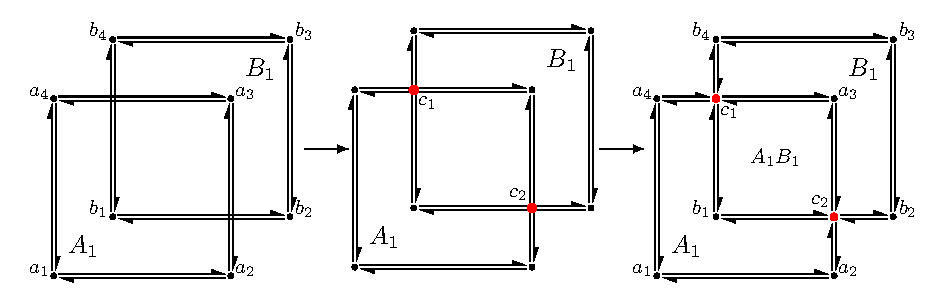
\includegraphics[width=\textwidth]{chapterSDCEL/dcel2/dcel2}
    \caption{Sequential computations of an overlay of two DCEL layers.}\label{fig:dcel_seq}
\end{figure}

Once the overlay structure of two DCELs is computed, queries like their intersection, union, difference, etc. (Figure \ref{fig:dcel_operators}) can be performed in linear time to the number of faces in the overlay. The space requirement for the overlay structure remains linear to the number of vertices, edges, and faces. Since an overlay is itself a DCEL, it can support the traditional DCEL operations (e.g., find the boundary of a face, access a face from an adjacent one, visit all the edges around a vertex, etc).

\begin{figure}
    \centering
    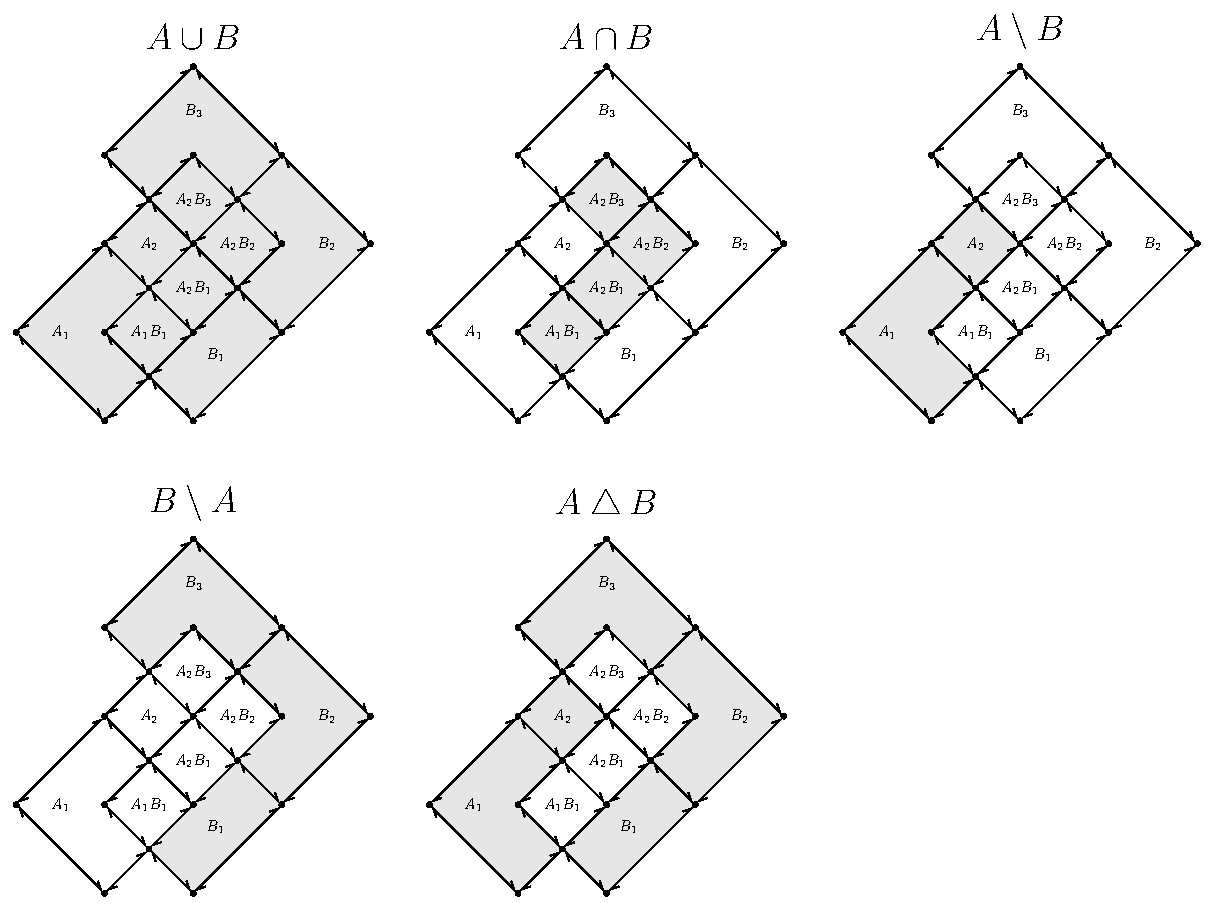
\includegraphics[width=\textwidth]{chapterSDCEL/dcel_operators/dcel_operators}
    \caption{Examples of overlay operators supported by DCEL; results are shown in gray.}
    \label{fig:dcel_operators}
\end{figure}

\section{Scalable Overlay Construction}\label{sec:methods}
This section presents the construction of overlay DCELs, assuming 2D polygons as input. The overlay computation depends on the size of the input DCELs and the size of the resulting overlay. The DCEL of a planar subdivision $S_1$ has size $O(n_1)$ where $n_1$ = $\Sigma (vertices_1 + edges_1 + faces_1$).  The sequential algorithm constructing the overlay of $S_1$ and $S_2$ takes $O(n \log n + k \log n)$ time, where $n = n_1 + n_2$ and $k$ is the size of their overlay.  Note that $k$ depends on how many intersections occur between the input DCELs, which can be very large \cite{berg_computational_2008}.

While the sequential algorithm is efficient with small DCEL layers, it suffers when the input layers are large and have many intersections. For example, creating the overlay between the DCELs of two census tracts (from years 2000 and 2010) from California (each with 7K-8K polygons and 2.7M-2.9M edges) took about 800sec on an Intel Xeon CPU at 1.70GHz  with 2GB of memory (see Section \ref{sec:experiments}). With DCELs corresponding to the whole US, the algorithm crashed.

Nevertheless, the overlay computation can take advantage of \textit{\textbf{partitioning}} (and thus parallelism) by observing that the edges in a given area of one input layer can only intersect with edges from the same area in the other input layer. One can thus spatially partition the two input DCELs and then compute the overlay within each cell; such computations are independent and can be performed in parallel. While this is a high-level view of our scalable approach, there are various challenges, including how to deal with edges that cross cells, how to manage the extra complexity introduced by \textit{orphan} holes (i.e., when holes and their polygons are in different cells), how and where to combine partition overlays into a global overlay, as well as how to balance the computation if one layer is much larger than the other.

\subsection{Partition Strategy} \label{sec:pstrategies}

%% Extension
% \subsubsection{Kd-tree Partition Strategy} %\label{sec:kdtreestrategy}
% In Section \ref{sec:pstrategies}, we use the quadtree spatial index as the baseline for our partitioning strategy. The quadtree follows a space-oriented approach, as it does not consider the content of each cell when determining potential splits. In contrast, kd-tree-based partitioning employs a data-oriented approach by sorting and selecting the midpoint within a cell to guide the placement of splits for future child nodes.
% 
% Building and populating the kd-tree partitioning follows a process similar to that of the quadtree. First, a kd-tree is constructed from a sample representing 1\% of the input data to define the tree’s structure, where the leaves represent the partition’s cells. The input data is then fed into this kd-tree structure, with each edge assigned to the leaf cell containing its boundaries. After partitioning, the local DCELs for each layer are constructed, and the overlay operation is performed within each cell as described in Section \ref{sec:pstrategies}.
% 
% Section \ref{sec:extension_experiments} will compare two partitioning strategies, the one presented in \ref{sec:pstrategies} based on the quadtree (i.e. space-oriented) and one on the kd-tree (i.e. data-oriented) indexes.  Note that both tree-based data partitioning involves shuffling all edges; this however, happens only once. Our experimental evaluation (see Section \ref{sec:comparison}) shows that the data-oriented approach leads to better performance.

While a simple grid could be used to divide the spatial area, our early experiments demonstrated that this approach leads to unbalanced cells, with some containing significantly more edges than others, negatively impacting overall performance.  Therefore, an advanced partitioning strategy is better since it adapts to skewed spatial distributions and helps assign a similar number of edges to each cell. In particular, we used two partitioning strategies, one based on the quadtree (i.e. space-oriented) and one on the kd-tree (i.e. data-oriented) indexes.

Note that such tree-based data partitioning involves shuffling all edges; this however, happens only once.  Our experimental evaluation (see Section \ref{sec:comparison}) shows that the data-oriented approach leads to better performance. Nevertheless, in describing the various challenges (orphan cells and holes, overlay evaluation, and optimizations) we use the quadtree-based partition since its well-defined space-oriented partitioning makes the presentation easier.

\subsubsection{Quadtree Partition Strategy}
\label{sec:strategy}

The main idea of the quadtree partition strategy is to split the area covered by the input layers into non-overlapping cells, which can then be processed independently.  While a simple grid could be used to divide the spatial area, our early experiments demonstrated that this approach leads to unbalanced cells, with some containing significantly more edges than others, negatively impacting overall performance.  In the rest we assume that the partitioning is performed using a quadtree index wich adapts to skewed spatial distributions and helps to assign a similiar number of edges to each cell.

The overall approach can be summarized in the following steps: (i) Partition the input layers into the index cells and build local DCEL representations of them at each cell, and (ii) Compute the overlay of the DCELs at each cell. Overlay operators and other functions can be run over the local overlays, and local results are collected to generate the final answer.

Note that each input layer is given as a sequence of polygon edges, where each edge record contains the coordinates of the edge's vertices (origin and target vertex) as well as the polygon id and a hole id in the case that an edge belongs to a hole inside of a polygon. We assume there are no overlapping or stacked polygons in the dataset.

To quickly build the partitioning quadtree structure, we build a quadtree from a sample taken from the edges of each layer (1\% of the total number of edges in that layer). We then use the leaves of that quadtree as the cells (partitions) of the partitioning scheme. These cells will be used to assign the edges of each input layer. Populated cells are then distributed to the available nodes for processing the overlay operations.

To support the creation of the quadtree we use the sampling functionalities provided in the Apache Sedona, an extension available on the Apache Spark platform. It allows the user to provide a parameter for the number of quadtree leaves; using this parameter as an approximation, it builds a quadtree; it should be noted that the actual number of leaves created is typically larger than the parameter provided by the user. The number of user-requested leaves and the size of the sample are used to compute the maximum number of entries per node (capacity) during the construction of the tree.  If the node capacity is exceeded, the node is divided into four child nodes with an equal spatial area, and its data is distributed among the four child nodes.  If any child node has exceeded its capacity, it is further divided into four nodes recursively and so on, until each node holds at most its computed \textit{capacity}.

After creating the quadtree from the sample, we use its leaf nodes as the partitioning cells for each layer. Each input layer file is then read from the disk, and \textit{all} its edges are inserted into the appropriate cells of the partitioning structure. Note that the partitioning structure created from the sample is now fixed; no more cells are created when the layer edges are assigned to cells. In the rest, we use the term cell and partition interchangeably.

For this approach to work, it is important that each cell can compute its two DCELs independently. An edge can be fully contained in a cell, or it can intersect  the cell's boundary. In the second case, we copy this edge to all cells where it intersects, but within each cell, we use the part of the edge that lies fully inside the cell. Figure \ref{fig:partition_strategy} shows an example where four cells and two edges of the upper polygon from layer A cross the cell borders.  Such edges are clipped at the cell borders, introducing new edges (e.g., edges $\alpha^{\prime}$ and $\alpha^{\prime \prime}$ in the Figure \ref{fig:partition_strategy}). Similarly, a polygon that crosses over a cell is clipped to the cell by introducing \textit{\textbf{artificial}} edges on the cell's border (see face $A_2$ in cell 3 of Figure \ref{fig:partition_strategy}). Such artificial edges are shown in red in the figure. This allows for the creation of a smaller polygon that is contained within each cell.

\begin{figure}
    \centering
    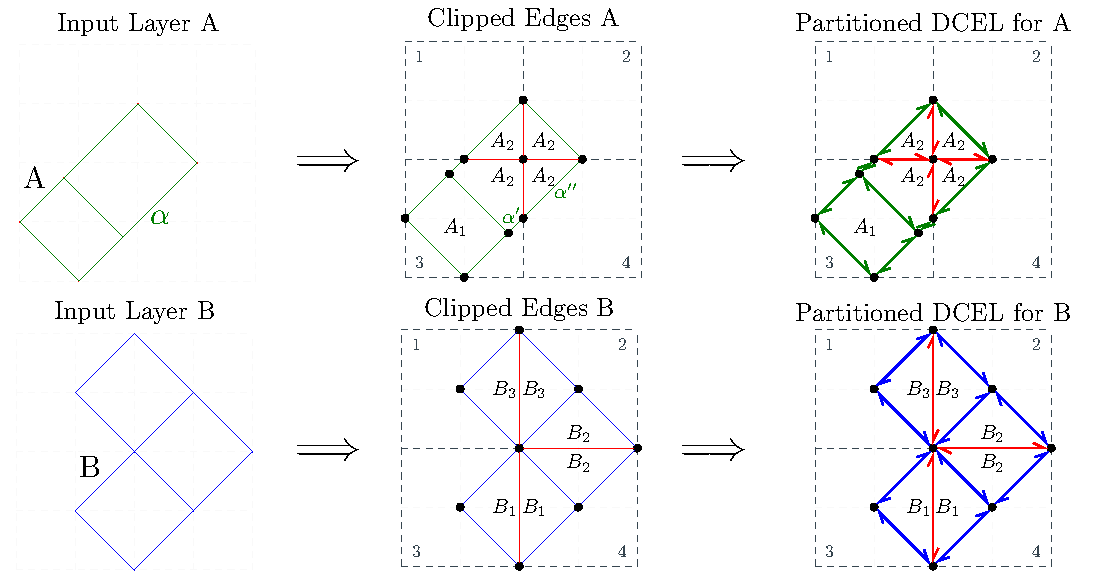
\includegraphics[width=\textwidth]{chapterSDCEL/partition_schema/PolygonsParted}
    \caption{Partitioning example using input layers A and B over four cells.} \label{fig:partition_strategy}
\end{figure}

For example, polygon $A_2$ is clipped into four smaller polygons as it overlaps all four cells. The clipping of edges and polygons ensures that each cell has 
all the needed information to complete its DCEL computations. As such computations can be performed independently, they are sent to different worker nodes to be 
processed in parallel. The assignment is delegated to the distributed framework (i.e., Apache Spark). 

Once a cell is assigned to a worker node, the sequential algorithm is used to create a DCEL for each layer (using the cell edges from that layer and any 
artificial edges, vertices, and faces created by the clipping procedures above) and then compute the corresponding (local) overlay for this cell. Using the 
example from Figure \ref{fig:partition_strategy}, Figure \ref{fig:overlay_partition} depicts an overview of the process for creating a local overlay DCEL inside 
cell 2. Similarly, Figure \ref{fig:distributed_dcel} shows all local overlay DCELs computed at each cell (artificial edges are shown in red). 

\begin{figure}
    \centering
    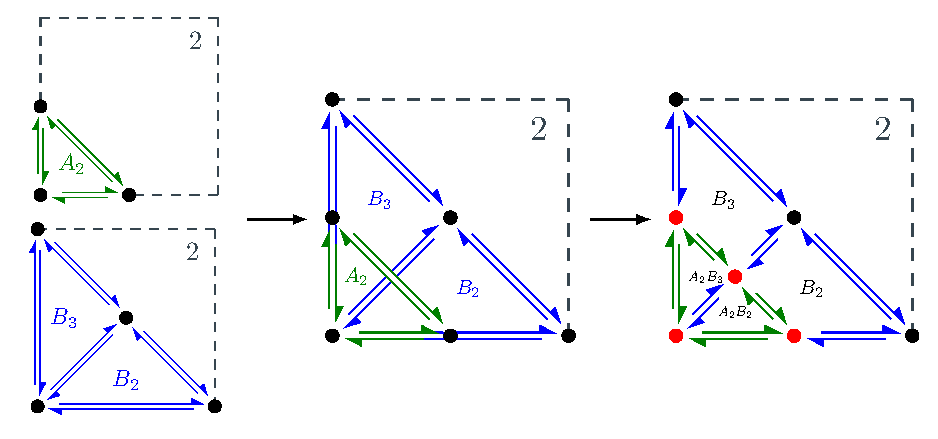
\includegraphics[width=\linewidth]
    {chapterSDCEL/overlay_partition/overlay_partition}
    \caption{Local overlay DCEL for cell 2.}\label{fig:overlay_partition}
\end{figure}

\begin{figure}
    \centering
    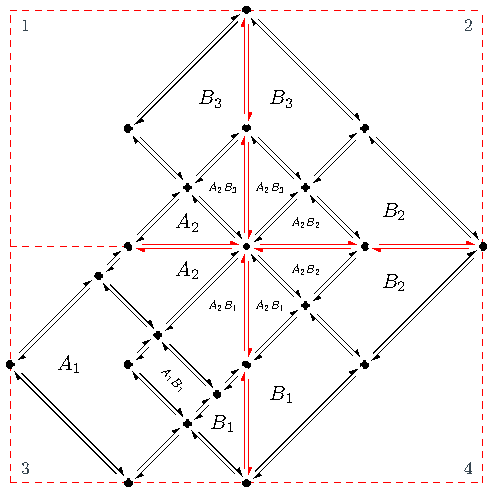
\includegraphics[width=0.75\linewidth]{chapterSDCEL/distributed_dcel/distributed_dcel}
    \caption{Result of the local overlay DCEL computations.}\label{fig:distributed_dcel}
\end{figure}

%%%
% Orphan cell and orphan hole problems...
%%%
Nevertheless, the partitioning creates two problems (not present in the sequential environment) that need to be addressed. 
The first is the case where a cell is empty; it does not intersect with (or contain) any regular edge from either layer. A regular edge is not part of a hole.
This empty cell does not contain any label, and thus, we do not know which face it may belong to. We term this as the \textbf{\textit{orphan cell}} problem.
An example is shown in Figure \ref{fig:orphan_cells}, which depicts a face (from one of the input layers) whose boundary goes over many quadtree cells; orphan 
cells are shown in grey. 

Note that an orphan cell may contain a hole (see Figure \ref{fig:orphan_cells}). In this case, the original label of the face where the hole belongs (and 
reported in the hole's edges) may have changed during the overlay computation (because it overlapped with a face from the other layer). However, this new label 
has not been propagated to the hole edges.
We term this as the \textbf{\textit{orphan hole}} problem. For simplicity, we focus on the case where a hole is within one orphan cell, but in the general case, 
a hole can split among many such cells.

The issue with both `orphan' problems is the missing labels. In section \ref{sec:anomalies}, we propose an algorithm that correctly labels an orphan cell. If 
this cell contains a hole, the new label is also used to update the hole edges. 

\subsubsection{Kd-tree Partition Strategy} \label{sec:kdtreestrategy}

The kd-tree based partitioning is a data-oriented approach because it sorts and picks the middle point inside a cell to locate the split of the future children. 1\% of the input data is used to build a kd-tree and extract the tree's structure.  The leaves of this structure are the partition's cells.  We feed the input data into the generated kd-tree structure to assign each edge to the leaf cell that has the edge within its boundaries.  After the partitioning is done, the construction of the local DCELs for each layer and the overlay operation is performed in each local cell in the same fashion as described in section \ref{sec:strategy}. 


\subsection{Labeling Orphan Cells and Holes} \label{sec:anomalies}
Assuming a quadtree-based partitioning, to find the label of an orphan cell, we propose an algorithm that recursively searches the space around the orphan cell
until it identifies a nearby cell that contains an edge(s) of the face that includes the orphan cell and thus acquire the appropriate label information. The 
quadtree index accommodates this search. Two observations are in order: (1) each cell is a leaf of the quadtree index (by construction), and (2) each cell has a 
unique id created by the way this cell was created; this id effectively provides the \textit{lineage} (unique path) from the quadtree root to this leaf.

Recall that the root has four possible children (typically numbered as 0,1,2,3 corresponding to the four children NW, NE, SW, and SE). The lineage is the 
sequence of these numbers in the path to the leaf. For example, the lineage for the shaded orphan cell in Figure \ref{fig:orphan_cells}(a) is 03. Further, note 
that the quadtree is an unbalanced structure, having more deep leaves where there are more edges. Thus, higher leaves correspond to larger areas, and deeper 
leaves correspond to smaller areas (since a cell split is created when a cell has more edges than a threshold).

\begin{figure}
    \centering
    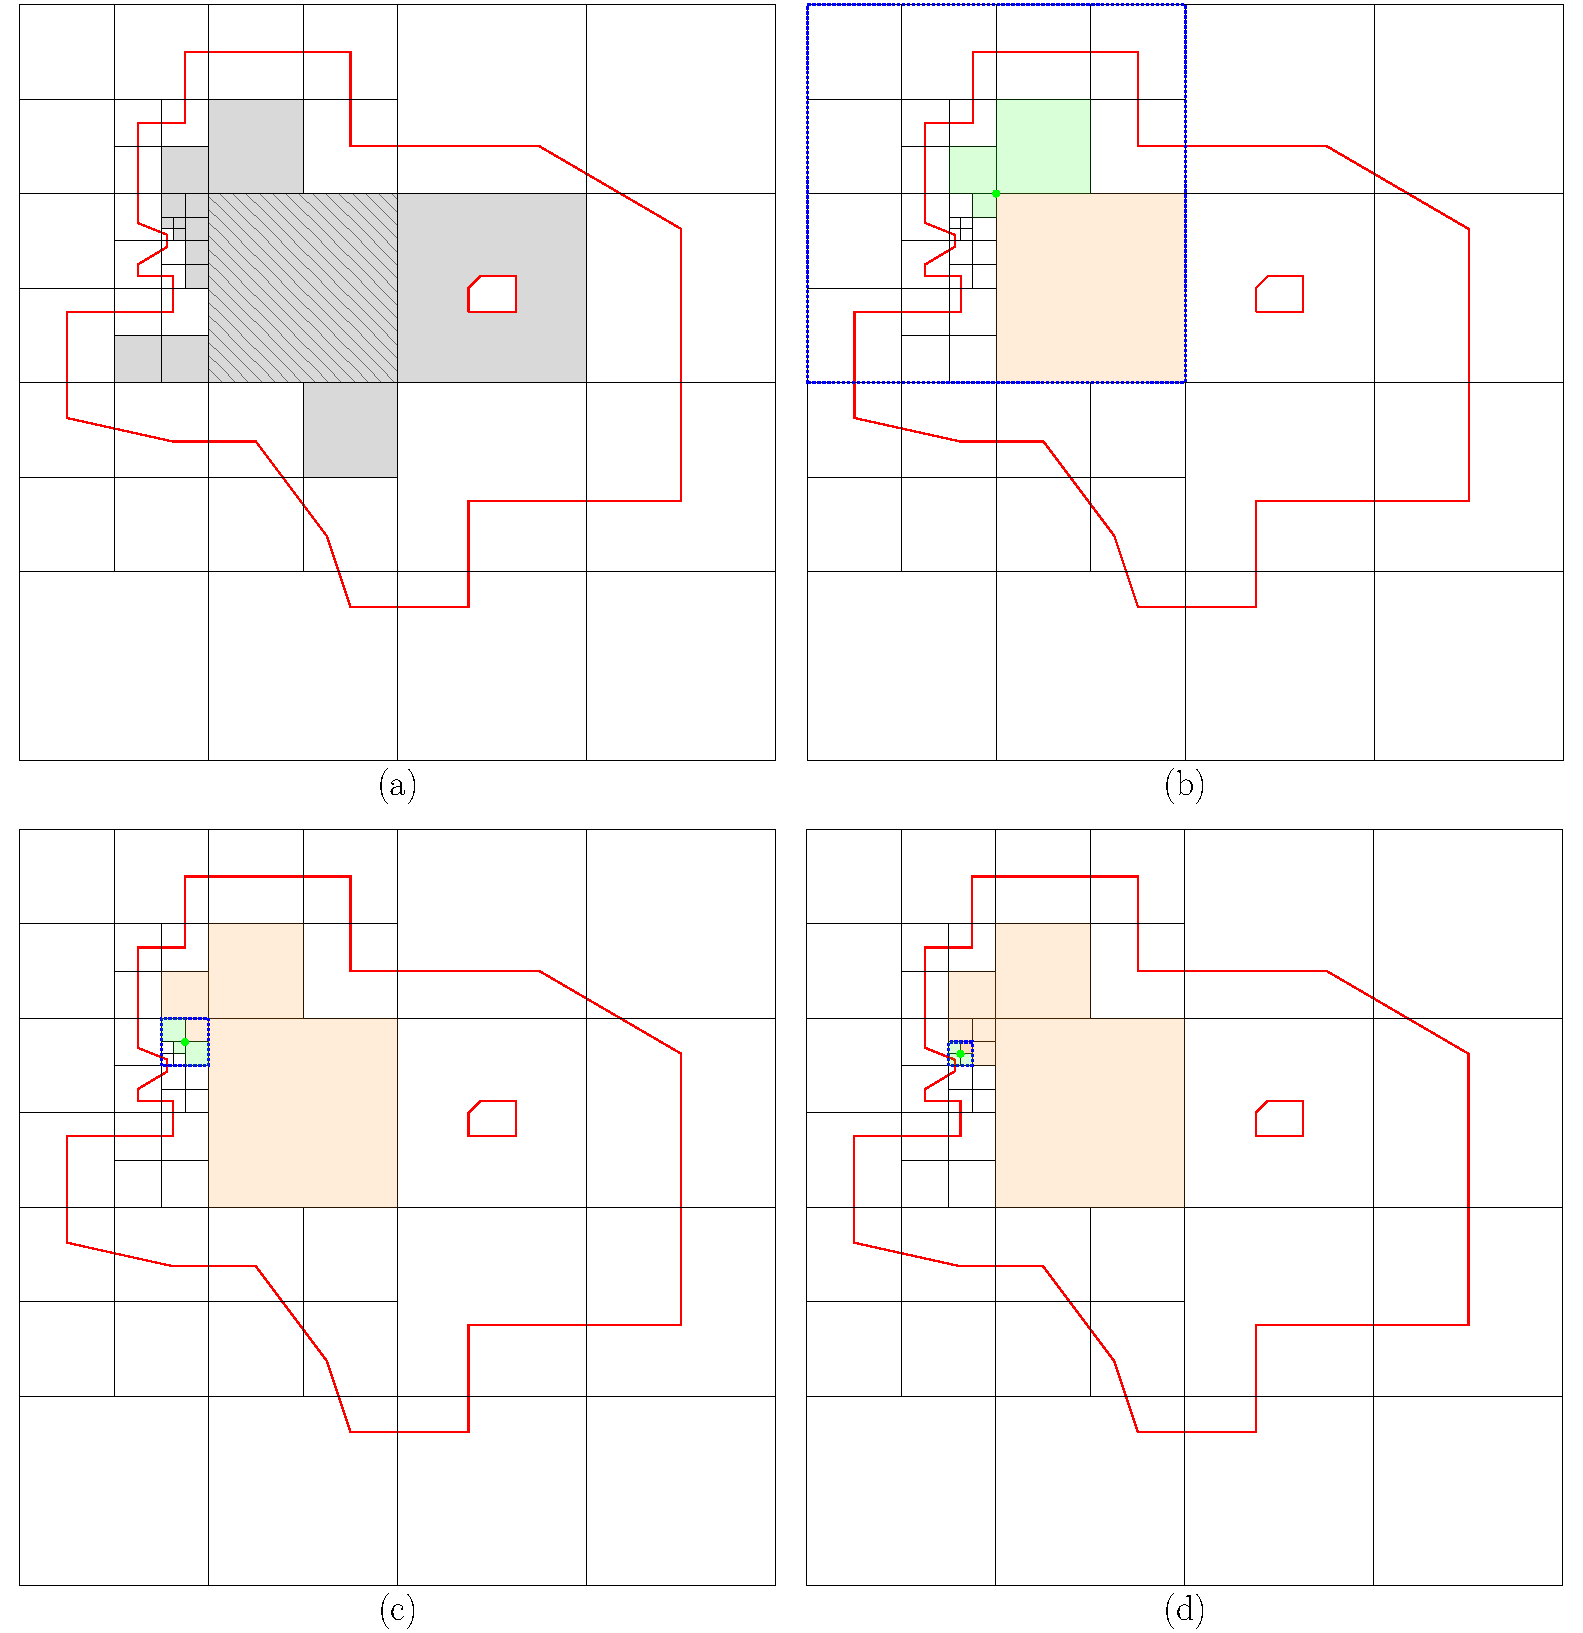
\includegraphics[width=\textwidth]{chapterSDCEL/orphan_cells/orphan_cells}    
    \caption{(a) Empty cell and hole examples; (b)-(c)-(d) show three iterations of the proposed solution.} \label{fig:orphan_cells}
\end{figure}

After identifying an orphan cell, the question
is where to search for a cell containing an edge. The following Lemma applies:

\begin{lemma} %\label{lem:cells}
Given an orphan cell, one of its siblings at the same quadtree level must contain a regular edge (directly or in its subtree). 
\end{lemma}

This lemma arises from the simple observation that if all three siblings of an orphan cell are empty, then there is no reason for the quadtree to make this split and create these four siblings. Based on the lemma, we know that at least one of the three siblings of the orphan cell can lead us to a cell with an edge.   However, these siblings may not be cells (leaves). Instead of searching each one of them in the quadtree until we reach their leaves, we want a way to quickly reach their leaves. To do so, we pick the centroid point of the orphan cell's parent (which is also one of the corners of the orphan cell).

For example, the parent centroid for the orphan cell 03 is the green point in Figure \ref{fig:orphan_cells}(b). We then query the quadtree to identify which cells (leaves, one from each sibling) contain this point. We check whether these cells contain an edge; if we find such a cell, we stop (and use the label in that cell). If all three cells are orphans, we need to continue the search. An example appears in Figure \ref{fig:orphan_cells}(b), where all three cells (green in the figure) are also orphans.

We first check if any of these orphan cells is a sibling (has the same parent) of the original cell. In this case that sibling is also a leaf (i.e. it does not have a subtree) and does need to be explored.  The remaining orphans are therefore at a lower level than the original orphan cell, which means they come from a sibling that has been split because of some edge. The algorithm picks any of the remaining orphan cells to continue. In Figure \ref{fig:orphan_cells}(b) all three leaves (green orphan cells) are at a lower level than the original orphan cell.

One can use different heuristics to pick which of the remaining leaves to use. Below, we consider the case where we use the deepest cell (i.e., the one with the longest lineage) among the leaves. This is because we expect this to lead us to the denser areas of the quadtree index, where there is more chance to find cells with edges. Figure \ref{fig:orphan_cells} shows a three-iteration run of the algorithm.

During the search process, we keep any orphan cells we discover; after a cell with an edge (non-orphan cell) is found, the algorithm stops and labels the original orphan cell and any other orphan cells retrieved in the search with the label found in the non-orphan cell. Note that if the non-orphan cell contains many labels (because different faces pass through it), we assign the label of the face that contains the original centroid.

The pseudo-code of the search process can be seen in Algorithms \ref{alg:one} and \ref{alg:two}. Another heuristic we used that is not described here is to follow the highest among the three orphan cells; i.e. the one with the shorter lineage since this has a larger area and will thus help us cover more empty space and possibly reach the border of the face faster.

{\ssp
\begin{algorithm}\caption{\textsc{getNextCellWithEdges} algorithm}\label{alg:one}
    \begin{algorithmic}[1]
    \Require a quadtree $\mathcal Q$ and a list of cells $\mathcal M$.
    \Function{ getNextCellWithEdges }{ $\mathcal Q$, $\mathcal M$ }
        \State $\mathcal C \gets $ orphan cells in $\mathcal M$
        \ForEach{ $orphanCell$ in $\mathcal C $ }
            \State initialize $cellList$ with $orphanCell$ 
            \State $nextCellWithEdges \gets nil$
            \State $referenceCorner \gets nil$
            \State $done \gets false$
            \While{ $\neg done$ } 
                \State $c \gets $ last cell in $cellList$ 
                \State $cells, corner \gets \textsc{getCellsAtCorner}(\mathcal Q, c)$ 
                \ForEach{$cell$ in $cells$}
                    \State $nedges \gets$ get edge count of $cell$ in $\mathcal M$ 
                    \If{ $nedges > 0$ }
                        \State $nextCellWithEdges \gets cell$
                        \State $referenceCorner \gets corner$
                        \State $done \gets true$
                    \Else
                        \If{$cell.level < orphanCell.level$}
                            \State add $cell$ to $cellList$
                        \EndIf
                    \EndIf
                \EndFor
            \EndWhile
            \ForEach{ $cell$ in $cellList$ }
                \State \textbf{output}($cell$, \\
                \hspace{2.5cm} $nextCellWithEdges$, $referenceCorner$)
                \State remove $cell$ from $\mathcal C$
            \EndFor
        \EndFor
    \EndFunction
    \end{algorithmic}
\end{algorithm}
}

{\ssp
\begin{algorithm} \caption{\textsc{getCellsAtCorner} algorithm}\label{alg:two}
    \begin{algorithmic}
    \Require a quadtree $\mathcal Q$ and a cell $c$.
    \Function{ getCellsAtCorner }{ $\mathcal Q$, $c$ }
        \State $region \gets $ quadrant region of c in $c.parent$
        \Switch{ $region$ }
            \Case{ `SW' }
                \State $corner \gets$ left bottom corner of $c.envelope$
            \EndCase
            \Case{ `SE' }
                \State $corner \gets$ right bottom corner of $c.envelope$
            \EndCase
            \Case{ `NW' }
                \State $corner \gets$ left upper corner of $c.envelope$
            \EndCase
            \Case{ `NE' }
                \State $corner \gets$ right upper corner of $c.envelope$
            \EndCase
        \EndSwitch
        \State $cells \gets$ cells which intersect $corner$ in $\mathcal Q$
        \State $cells \gets cells - c$ 
        \State $cells \gets$ sort $cells$ on basis of their depth 
        \State \Return{ ($cells$, $corner$) }
    \EndFunction
    \end{algorithmic}
\end{algorithm}
}

To determine the worst-case performance of the search algorithm, consider that for an orphan cell, the algorithm performs three point quadtree queries to find the sibling leaves containing the centroid. It then selects one of these leaves and repeats the process, querying three points for a new centroid within the siblings of the selected leaf. This causes the algorithm to explore progressively deeper into the quadtree. In the worst case, the longest path in the quadtree could result in a time complexity of $O(N)$. However, in the average case, when the quadtree is balanced, the complexity is logarithmic.

\subsection{Answering global overlay queries} %\label{sec:reduce}
Using the local overlay DCELs, we can easily compute the global overlay DCEL; for that, we need a reduce phase, described below, to remove artificial edges, and 
concatenate split edges from all the faces. Using the local overlay DCELs, we can also compute in a scalable way global operators like intersection, difference, 
symmetric difference, etc. For these operators, there is first a map phase that computes the specific operator on each local DCEL, followed by a reduce phase to 
remove artificial edges/added vertices.
Figure \ref{fig:overlay_operator} shows how the intersection overlay operator ($A \cap B$) is computed, starting with the local DCELs for four cells in Figure 
\ref{fig:overlay_operator}(a). First, each cell computes the intersection using its local overlay DCEL as shown in Figure \ref{fig:overlay_operator}(b). This is 
a map operation to identify overlay faces that contain both labels from layer A and layer B. Each cell can then report every such face that does not include any 
artificial edges, like face $A_1B_1$ in Figure \ref{fig:overlay_operator}(b); note that these faces are fully included in the cell. 

Using a reduce phase, the remaining faces are sent to a master node; in our implementation, it would be the driver node of the spark application that will (i) remove the artificial edges, shown in red in the figure and (ii) concatenate edges that were split because they were crossing cell borders. This is done by pairing faces with the same label and concatenating their geometries by removing the artificial edges and vertices added during the partition stage, for example, the two faces with label $A_2B_1$ from two different cells in Figure \ref{fig:overlay_operator}(b) were combined into one face in Figure \ref{fig:overlay_operator}(c). While the extra vertex was also removed. In section \ref{sec:optimizing}, we discuss techniques to optimize the reduce process of combining faces.

For symmetric difference, $A \bigtriangleup B$, the map phase filters faces whose label is a single layer (A or B). For the difference, $A \setminus B$, it 
filters faces with label A. For union $A \cup B$, all faces in the overlay structure are retrieved. 

\begin{figure}
    \centering
    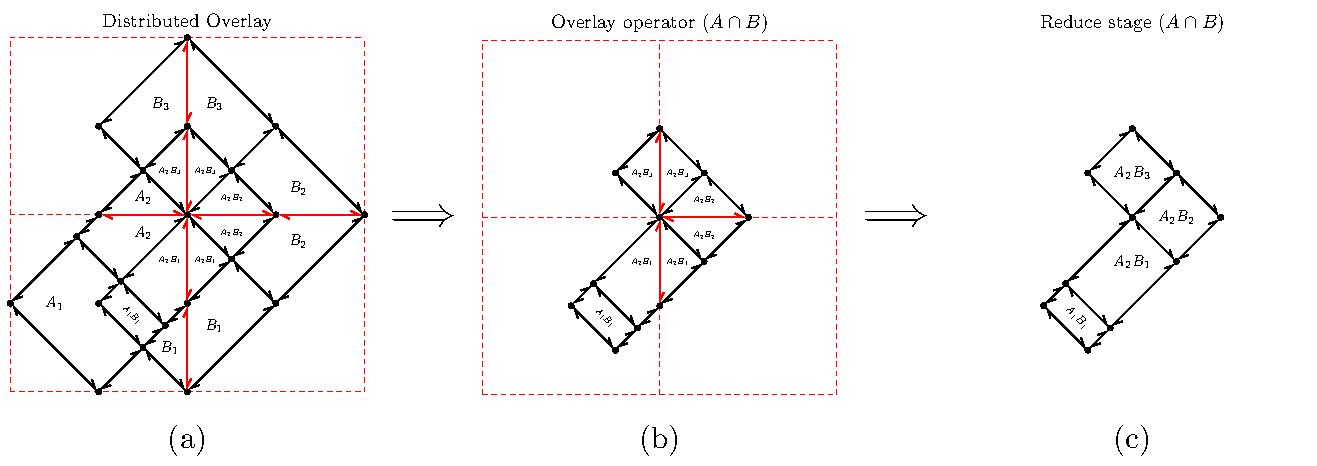
\includegraphics[width=\linewidth]{chapterSDCEL/overlay_operator/overlay_operator}
    \caption{Example of an overlay operator querying the distributed DCEL.} \label{fig:overlay_operator}
\end{figure}

\section{Overlay evaluation optimizations}\label{sec:alternative_methods}
We now focus on the different optimization aspects regarding the best approach to compute the boundaries of faces that span over different cells and how to mitigate the issues of layers with an unbalanced number of edges.

\subsection{Optimizations for faces spanning multiple cells}\label{sec:optimizing}

The naive reduce phase described above has the potential for a bottleneck since all faces, which can be a very large number, are sent to one worker node. From a distributed perspective, this process follows a typical MapReduce pattern. In the map phase, each worker node identifies and reports faces that are fully contained within its boundaries, as well as segments of faces that may need to be concatenated with segments reported by other nodes. These face segments are then sent to a master node, incurring communication costs as the master must wait for all nodes to report their segments. In the reduce phase, the master node groups the segments by face ID, sorts them, and concatenates the parts to form complete, closed faces.  One observation is that faces from different concatenated cells are in contiguous cells. This implies that faces from a particular cell will be combined with faces from neighboring cells. We will use this spatial proximity property to reduce the overhead in the central node.

We thus propose an alternative where an intermediate reduce processing step is introduced. In particular, the user can specify a level in the quadtree structure, measured as the depth from the root, that can be used to combine cells together.  While it may be challenging to predetermine an optimal level, it can be estimated based on the input size or the number of partitions. Moreover, Section \ref{sec:overlay_optimization} offers recommendations for suitable values and alternative approaches.  Given level \textit{i}, the quadtree nodes in that level (at most $4^i$) will serve as intermediate reducers, collecting the faces from all the cells below that node. Note: level 0 corresponds to the root, which is the naive method where all the cells are sent to one node.

By introducing this intermediate step, it is expected that much of the reduce work can be distributed in a larger number of worker nodes. Nevertheless, there may be faces that cannot be completed by these intermediate reducers because they span the borders of the level $i$ nodes. Such faces still have to be evaluated in a master/root node.  From a Map-Reduce standpoint, this alternative functions similarly to the previous approach but introduces additional reduce operations at an intermediate level. However, this also introduces new synchronization points, as each intermediate reducer must wait for its workers to report potential face segments before processing them. The reducer then either reports completed faces or sends incomplete segments to the driver for further processing.

Clearly, picking the appropriate level is important. Choosing a level $i$, i.e., going to nodes lower in the quadtree structure, implies a larger number of intermediate reducers and, thus, higher parallelism. However, simultaneously, it increases the number of faces that would need to be evaluated by the master/root node. On the other hand, lowering $i$ reduces parallelism, but fewer faces will need to go to the master/root node.

We also examine another approach to deal with the bottleneck in the naive reduce phase. This approach re-partitions the faces using the label as the key. Such partitions represent small independent amounts of work since they only combine faces with the same label that are typically few. Partitions are then shuffled among the available nodes. The second approach effectively avoids the reduce phase; it has to account for the cost of the re-partitioning; however, as we will show in the experimental section, this cost is negligible.  From a distributed computing perspective, this alternative introduces a shuffle stage at the beginning, eliminating the need for a reduce operation. The shuffle ensures that all segments with the same face ID are placed in the same worker, allowing them to be processed and reported directly.

\subsection{Optimizing for unbalanced layers}\label{sec:unbalance}
During the overlay computation, finding the intersections between the half-edges is the most critical task. In many cases, the number of half-edges from each layer within a cell can be unbalanced; that is, one of the layers has many more half-edges than the other.

In our initial implementation, the input sets of half-edges within each cell were combined into a single dataset, initially ordered by the x-origin of each half-edge.  Then, a sweep-line algorithm is performed, scanning the half-edges from left to right (in the x-axis). This scanning takes time proportional to the total number of half-edges. However, if one layer has much fewer half-edges, the running time will still be affected by the cardinality of the larger dataset.

An alternative approach is to scan the larger dataset only for the x-intervals where we know that there are half-edges in the smaller dataset. To do so, we order the two input sets separately. We scan the smaller dataset in x-order and identify x-intervals occupied by at least one half-edge. For each x-interval, we then scan the larger dataset using the sweep-line algorithm. This focused approach avoids unnecessary scanning of the large dataset, for example, areas with no half-edges from the smaller dataset.

\section{Experimental Evaluation} \label{sec:experiments}
For our experimental evaluation, we used a 12-node Linux cluster (kernel 3.10) and Apache Spark 2.4. Each node has 9 cores (each core is an Intel Xeon CPU at 1.70GHz) and 2G memory.

The scalable approach was implemented over the Apache Spark framework.  From a Map-Reduce point of view the stages described in Section \ref{sec:methods} were implemented using several transformations and actions supported by Apache Spark.  For example, the partitioning and load balancing described in Section \ref{sec:pstrategies} was implemented using a quadtree, where its leaves were used to map and balance the number of edges that have to be sent to the worker nodes.  Mostly, map operations were used to process and locate the edges in the corresponding leaf to exploit proximity among them while at the same time dividing the amount of work among worker nodes.

Similarly, the edges at each partition were processed using chains of transformations at local level (see Section \ref{sec:methods}) followed by reducer actions to post-process incomplete faces which could span over multiples partitions and have to be combined or re-distributed to obtain the final answer.  In addition, the reduce actions were further optimized as described in Section \ref{sec:alternative_methods}.

\subsection{Evaluation datasets}
The details of the real datasets of polygons that we use are summarized in Table \ref{tab:sdcel_datasets}. The first dataset (MainUS) contains the complete Census Tracts for all the states on the US mainland for the years 2000 (layer A) and 2010 (layer B). It was collected from the official website of the United States Census Bureau \cite{census_tract}. The data was clipped to select just the states inside the continent. Something to note with this dataset is that the two layers present a spatial gap (which was due to improvements in the precision introduced for 2010). As a result, there are considerably more intersections between the two layers, thus creating many new faces for the DCEL.

\begin{table}
    \centering
    \caption{Evaluation Datasets}
    \label{tab:sdcel_datasets}
    \begin{tabular}{c c c c}
        \toprule
        Dataset & Layer & Number        & Number    \\
                &       & of polygons   & of edges  \\
        \midrule
        MainUS& Polygons for 2000 & 64983 & 35417146        \\
              & Polygons for 2010 & 72521 & 36764043        \\
        GADM  & Polygons for Level 2 & 160241 & 64598411    \\
              & Polygons for Level 3 & 223490 & 68779746    \\
        CCT   & Polygons for 2000 & 7028 & 2711639          \\
              & Polygons for 2010 & 8047 & 2917450          \\
        \bottomrule
    \end{tabular}
\end{table}

The second dataset, GADM - taken from Global Administration Areas \cite{gadm_data}, collects the geographical boundaries of the countries and their administrative divisions around the globe. For our experiments, one layer selects the States (administrative level 2), and the other has Counties (administrative level 3). Since GADM may contain multi-polygons, we split them into their individual polygons.

Since these two datasets are too large, a third, smaller dataset was created for comparisons with the sequential algorithm. This dataset is the California Census Tracts (CCT), a subset from MainUS for the state of California; layer A corresponds to the CA census tracts from the year 2000, while layer B corresponds to 2010. Below, we also use other states to create datasets with different numbers of faces.  To test the scalable approach, a sequential algorithm for DCEL creation was implemented based on the pseudo-code outlined in \cite{berg_computational_2008}.

\subsection{Overlay face optimizations}\label{sec:overlay_optimization}
We first examine the optimizations in Section \ref{sec:optimizing}. To consider different distributions of faces, for these experiments, we used 8 states from the MainUS dataset with different numbers of tracts (faces). In particular, we used, in decreasing order of number of tracts, CA, TX, NC, TN, GA, VA, PA, and FL. For each state, we computed the distributed overlay between two layers (2000 and 2010). For each computation, we compared the baseline; master at the root node, with intermediate reducers at different levels: $i$ varied from 4 to 10. 

Figure \ref{fig:overlay_tester} shows the results for the distributed overlay computation stage; after the local DCELs were computed at each cell. 
Note that for each state experiment, we tested different numbers of cells for the quadtree and reported the configuration with the best performance. To determine this, we sampled 1\% of the edges for each state and evaluated the best number of cells ranging from 200 to 2000. In most cases, the best number of cells was around 3000.
As expected, there is a trade-off between parallelism and how much work is left to the final reduce job. For different states, the optimal $i$ varied between levels 4 and 6. The figure also shows the optimization that re-partitions the faces by label id. This approach has actually the best performance. This is because few faces with the same label can be combined independently. This results in smaller jobs better distributed among the cluster nodes, and no reduce phase is needed. As a result, we use the label re-partition approach for the rest of the experiments to implement the overlay computation stage.

\begin{figure}
    \centering
    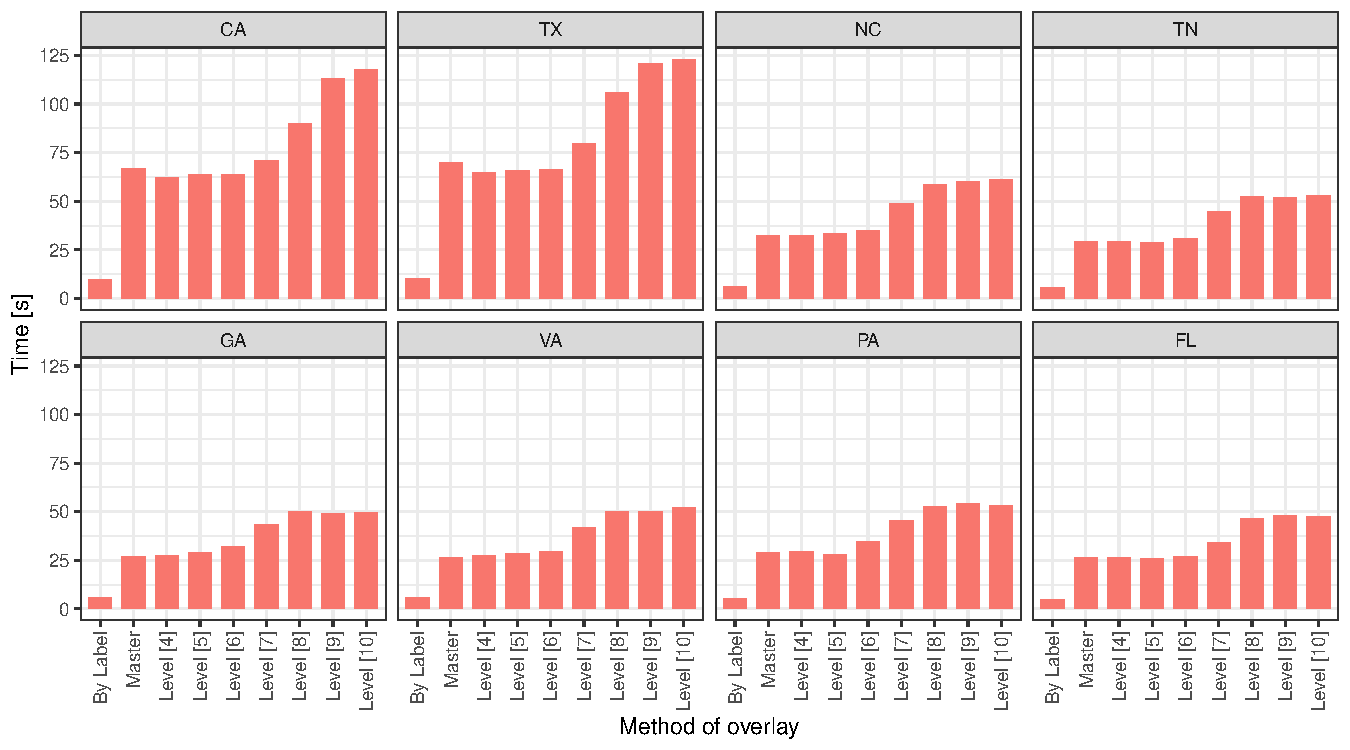
\includegraphics[width=\linewidth]{chapterSDCEL/OverlayTester/Overlay_Tester}
    \caption{Overlay methods evaluation.}\label{fig:overlay_tester}
\end{figure}

Finally we note that the overlay face optimizations involve shuffling of the incomplete faces. Table \ref{tab:percentages} shows the percentage of incomplete faces for three states, assuming 3000 cells. As it can be seen, the incomplete faces is small (in average 12.89\%) and moreover, for the \textit{By-Label} approach, this shuffling is parallelized.

\begin{table}
    \centering
    \caption{Percentages of edges in incomplete faces for three states} \label{tab:percentages}
    \begin{tabular}{cccc}
        \toprule
                & Number of & Edges in         &            \\
        Dataset & edges     & incomplete faces & Percentage \\
        \midrule
        CA &  47834 &  6339 & 13.25\% \\
        TX &  41227 &  4436 & 10.75\%\\
        FL &  24152 &  3547 & 14.68\%\\
        \bottomrule
    \end{tabular}
\end{table}

\subsection{Unbalanced layers optimization}
For these experiments, we compared the traditional sweep approach with the `filtered-sweep' approach that considers only the areas where the smaller layer has edges (Section \ref{sec:unbalance}).  To create the smaller cell layer, we picked a reference point in the state of Pennsylvania, from the MainUS dataset, and added 2000 census tracts until the number of edges reached 3K. We then varied the size of the larger cell layer in a controlled way: using the same reference point but using data from the 2010 census, and we started adding tracts to create a layer that had around 2x, 3x, ..., 7x the number of edges of the smaller dataset.

Since this optimization occurs per cell, we used a single node to perform the overlay computation within that cell. Figure \ref{fig:unbalance_tests}(a) shows the behavior of the two methods (filtered-sweep vs. traditional sweep) under the above-described data for the overlay computation stage.  Clearly, as the data from one layer grows much larger than the other layer, the filtered-sweep approach overcomes the traditional one.

\begin{figure}
    \centering
    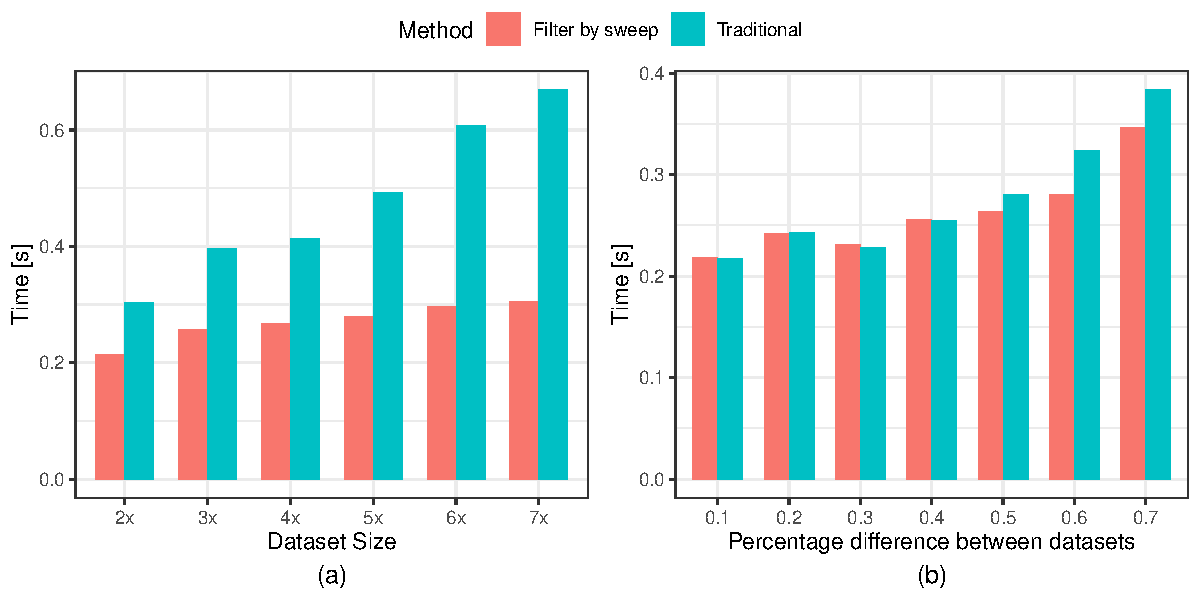
\includegraphics[width=\linewidth]{chapterSDCEL/UnbalanceTester/Unbalance_Tester}
    \caption{Evaluation of the unbalanced layers optimization.}\label{fig:unbalance_tests}
\end{figure}

We also performed an experiment where the difference in size between the two layers varies between 10\% and 70\%. For this experiment, we first identified cells from the GADM dataset where the smaller layer had around 3K edges. Among these cells, we then identified those where the larger layer had 10\%, 20\%, ... up to 70\% more edges. In each category, we picked 10 representative cells and computed the overlay for the cells in that category.

Figure \ref{fig:unbalance_tests}(b) shows the results; in each category, we show the average time to compute the overlay among the 10 cells in that category.  The filtered-sweep approach shows better performance as the percentage difference between layers increases. Based on these results, one could apply the optimization on those cells where the layer difference is significant (more than 50\%).  We anticipate that this optimization will be particularly beneficial for datasets where the two input layers contain many cells with significantly different edge counts.

\subsection{Varying the number of cells}
The quadtree configuration allows for performance tuning by setting the \textit{maximum capacity} of a cell. The quadtree continues splitting until this capacity is reached. There is an inverse relationship between the capacity and the number of leaf cells: a lower capacity results in more cells, while a higher capacity leads to fewer leaf cells. In skewed datasets, the quadtree may become unbalanced, with some branches splitting more frequently. As a result, the final number of partitions is not necessarily a multiple of four. In the figures, we round the number of leaf cells to the nearest thousand.

The number of cells affects the performance of our scalable overlay implementation, termed as SDCEL, since it relates to the average cell capacity given by the number of edges it could contain. As it was said before, a fewer number of cells implies larger cell capacity and thus more edges to process within each cell.  Complementary, creating more cells increases the number of jobs to be executed.

Figure \ref{fig:ca}(a) shows the SDCEL performance using the two layers of the CCT dataset while varying the number of cells from 100 to 15K (by multiple of 1000). Each bar corresponds to the time taken to create the DCEL for each layer and then combine them to create the distributed overlay. Clearly, there is a trade-off: as the number of cells increases, the SDCEL performance improves until a point where the larger number of cells adds an overhead. Figure \ref{fig:ca}(b) focuses on that area; the best SDCEL performance was around 7K cells.

In addition, Figure \ref{fig:ca}(a) shows the performance of the sequential solution (CGAL library) for computing the overlay of the two layers in the CCT dataset using one of the cluster nodes. Clearly, the scalable approach is much more efficient as it takes advantage of parallelism. Note that the CGAL library would crash when processing the larger datasets (MainUS and GADM).

\begin{figure}
    \centering
    \begin{tabular}{cc}
        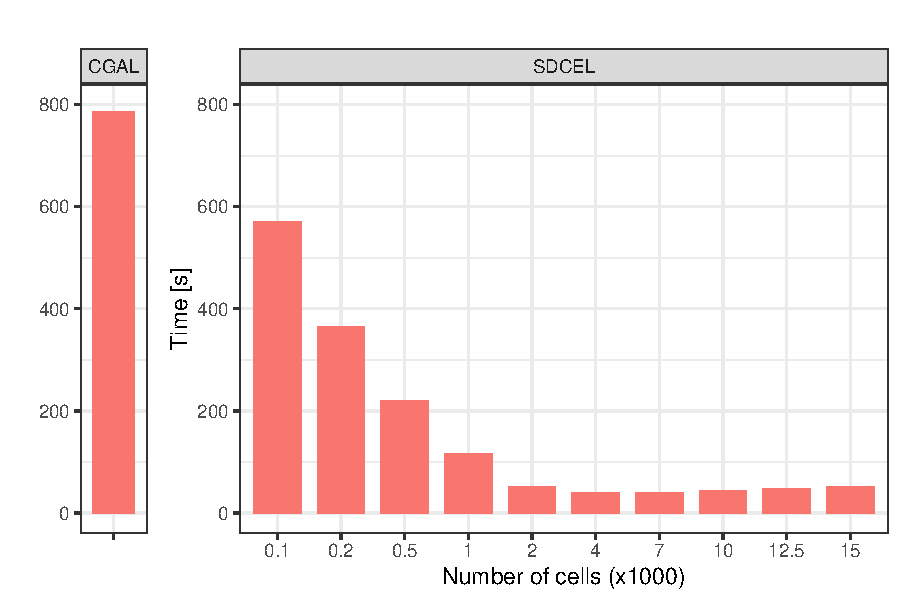
\includegraphics[width=0.50\linewidth]{chapterSDCEL/CA/CA} & 
        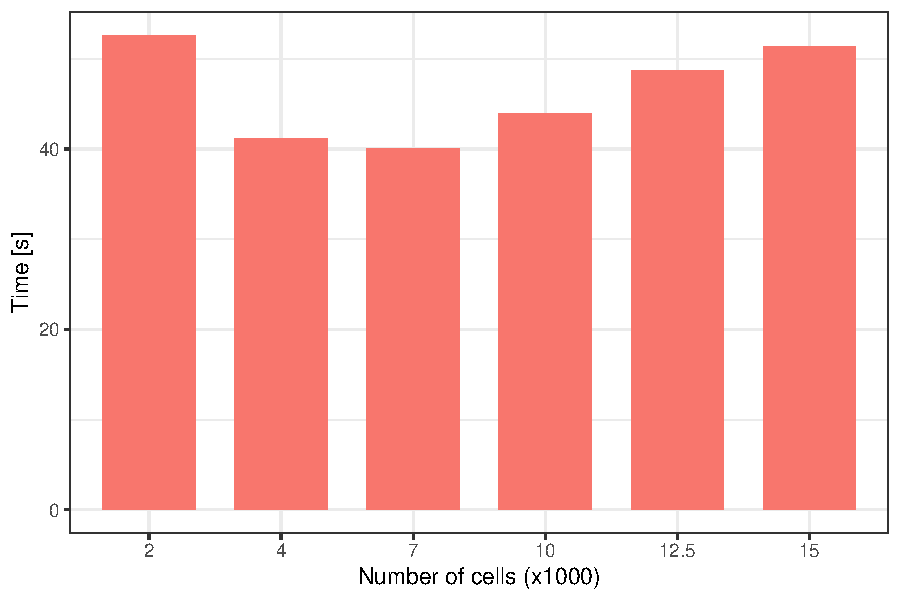
\includegraphics[width=0.45\linewidth]{chapterSDCEL/CA/CA_sample} \\
        (a) & (b)
    \end{tabular}
    \caption{SDCEL performance while varying the number of cells in the CCT dataset.} \label{fig:ca}
\end{figure}

\begin{figure}
    \centering
    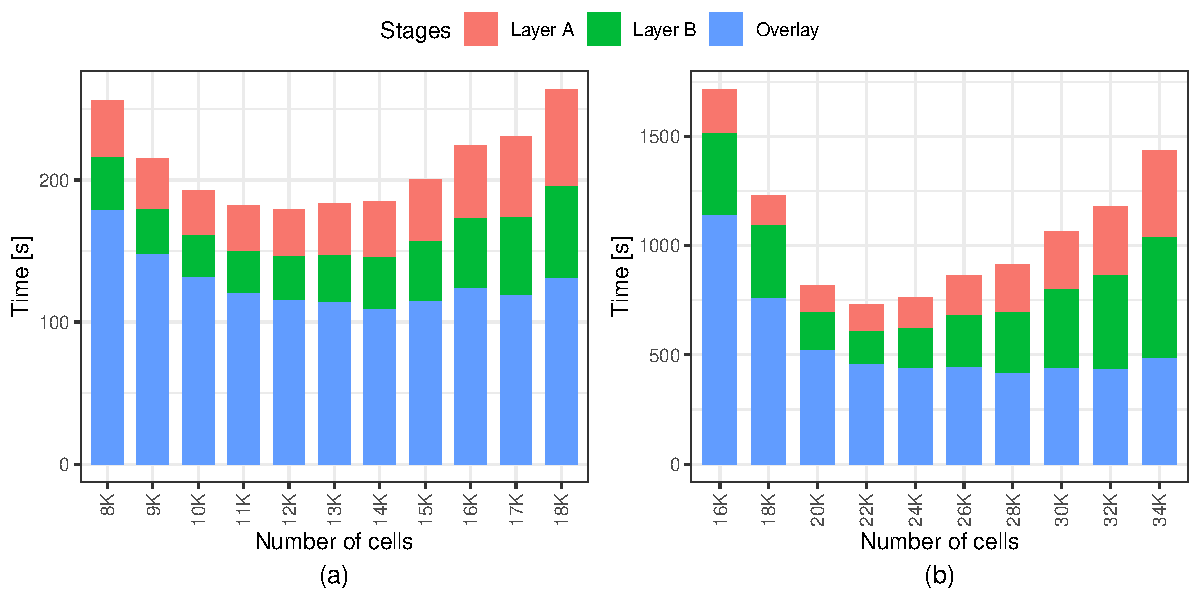
\includegraphics[width=\textwidth]{chapterSDCEL/Performance/Performance} 
    \caption{Performance with (a) MainUS and (b) GADM datasets.} \label{fig:mainus}
\end{figure}

Figure \ref{fig:mainus} shows the results when using the larger MainUS and GADM datasets, while again varying the number of cells parameter from 8K to 18K and from 16K to 34K, respectively. In this figure, we also show the time taken by each stage of the overlay computation.  This is, the time to create the DCEL for layer A, for layer B, and for their combination to create their distributed overlay. We can see a similar trade-off in each of the stages. The best performance is given when setting the number of cells parameter to 12K for the MainUS and 22K for the GADM dataset. Note that in the MainUS dataset, the two layers have a similar number of edges; as can be seen, their DCEL computations are similar.

Interestingly, the overlay computation is expensive since as mentioned earlier there are many intersections between the two layers. An interesting observation from the GADM plots is that layer B takes more time than layer A; this is because there are more edges in the counties than in the states. Moreover, county polygons are included in the (larger) state polygons. When the size of cells is small (i.e., a larger number of cells like in the case of 34K cells), these cells mainly contain counties from layer B. As a result, there are not many intersections between the layers in each cell, and the overlay computation is thus faster. On the other hand, with large cell sizes (smaller number of cells), the area covered by the cell is larger, containing more edges from states and thus increasing the number of intersections, resulting in higher overlay computation.

Additionally, Table \ref{tab:cell_stats} provides statistics on the cells. It shows that in larger datasets, an average cell size of approximately 3000 edges produces the best results. This cell size ensures a relatively small amount of data to transmit, which minimizes the impact on data shuffling and processing.  Table \ref{tab:orphans} presents the number of cells, original holes, and the orphan cells and holes generated after partitioning.

\begin{table}
    \centering
    \caption{Cell size statistics.}
    \label{tab:cell_stats}
    \begin{tabular}{ccccccc}
        \toprule
        Dataset & Min & 1st Qu. & Median & Mean & 3rd Qu. & Max   \\
        \midrule
        GADM    & 0   & 0       & 2768   & 3141 & 5052    & 16978 \\
        MainUS  & 0   & 1538    & 2582   & 2853 & 3970    & 10944 \\
        CCT     & 0   & 122     & 324    & 390  & 546     & 1230  \\
        \bottomrule
    \end{tabular}
\end{table}

\begin{table}
    \centering
    \caption{Orphan cells and orphan holes description}
    \label{tab:orphans}
    \begin{tabular}{c c c c}
        \toprule
                & Number   & Number   & Number of orphans   \\
        Dataset & of cells & of holes & (cell/holes) \\
        \midrule
        GADM  & 21970      & 1999     & 4310 \\
        MainUS& 12343      & 850      & 1069 \\
        CCT   & 7124       & 40       & 215  \\
        \bottomrule
    \end{tabular}
\end{table}

\subsection{Speed-up and Scale-up experiments} \label{sec:speed_scale}
The speed-up behavior of SDCEL appears in Figure \ref{fig:mainus_speed_scale}(a) (for the MainUS dataset) and in Figure \ref{fig:gadm_speed_scale}(a) (for the GADM dataset); in both cases, we show the performance for each stage. For these experiments, we varied the number of nodes to 3, 6, and 12 while keeping the input layers the same. Clearly, as the number of nodes increases, the performance improves. SDCEL shows good speed-up characteristics: as the number of nodes doubles from 3 to 6 and then from 6 to 12, the performance improves by almost half.

\begin{figure}
    \centering
    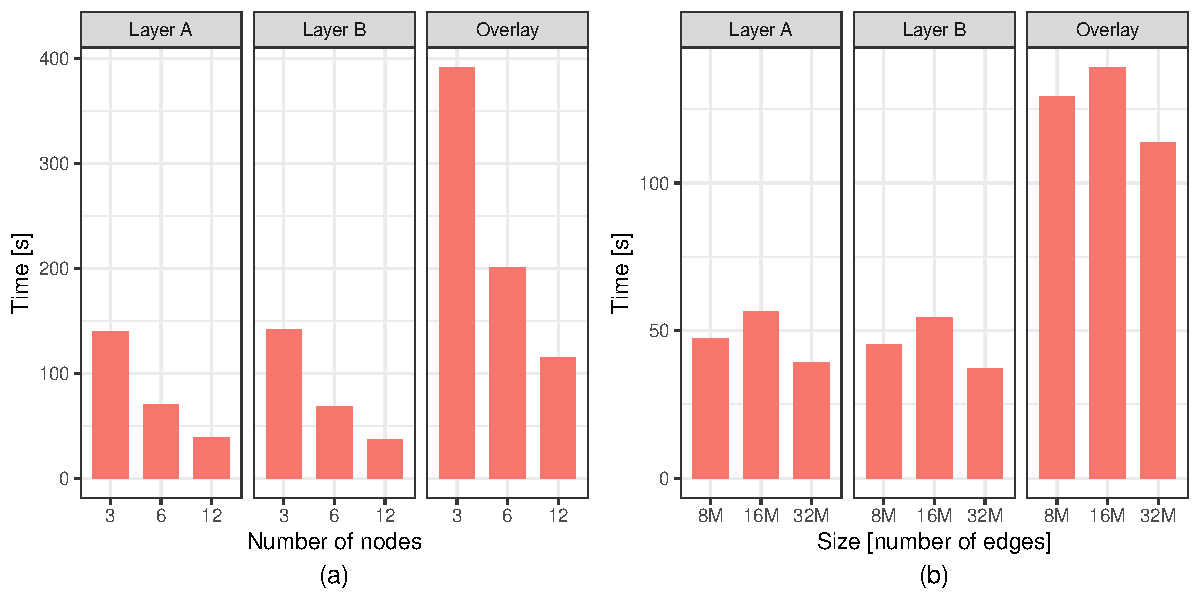
\includegraphics[width=\textwidth]{chapterSDCEL/MainUS_SS/MainUS_SS} 
    \caption{Speed-up and Scale-up experiments for the MainUS dataset.} 
\label{fig:mainus_speed_scale}
\end{figure}

\begin{figure}
    \centering
    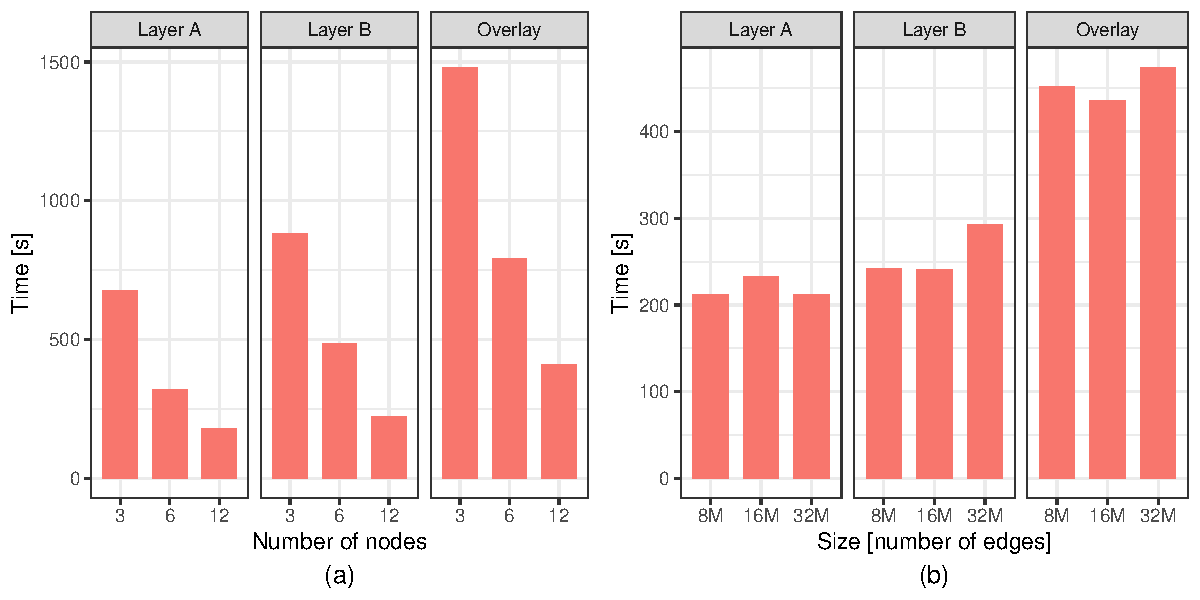
\includegraphics[width=\textwidth]{chapterSDCEL/GADM_SS/GADM_SS}
    \caption{Speed-up and Scale-up experiments for the GADM dataset.} \label{fig:gadm_speed_scale}
\end{figure}

To examine the scale-up behavior, we created smaller datasets out of the MainUS and similarly out of the GADM so that we could control the number of edges. To create such a dataset, we picked a centroid and started increasing the area covered by this dataset until the number of edges was closed to a specific number. For example, from the MainUS, we created datasets of sizes 8M, 16M, and 32M edges for each layer. We then used two layers of the same size as input to a different number of nodes while keeping the input-to-node ratio fixed. That is, the layers of size 8M were processed using 3 nodes, the layers of size 16M using 6 nodes, and the 32M using 12 nodes. We used the same process for the scale-up experiments with the GADM dataset. The results appear in Figure \ref{fig:mainus_speed_scale}(b) and Figure \ref{fig:gadm_speed_scale}(b).  Overall, SDCEL shows good scale-up performance; it remains almost constant as the work per node is similar (there are slight variations because we could not control perfectly the number of edges and their intersection).

%% Extension
%\subsection{Kd-tree versus quadtree performance} \label{sec:comparison}
%In order to compare the quadtree and the kd-tree partition strategies we analyze their performance during the construction of the spatial data structure which defines the cells that the partition will use based on the sample, the cost of partitioning; populating the cells with the full datasets, and the overall time to complete the phases of the overlay operation using each partitioning approach.  We use the datasets of MainUS and GADM described in Table \ref{tab:datasets}.

% \begin{figure}
%     \centering
%     \begin{tabular}{cc}
%         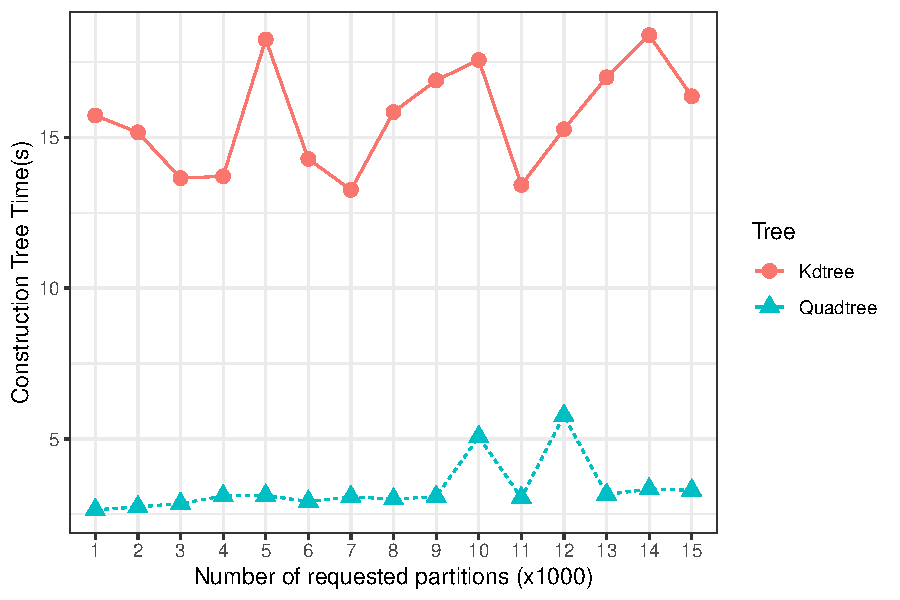
\includegraphics[width=0.49\linewidth]{chapterSDCEL/K_Creation_US.pdf} & 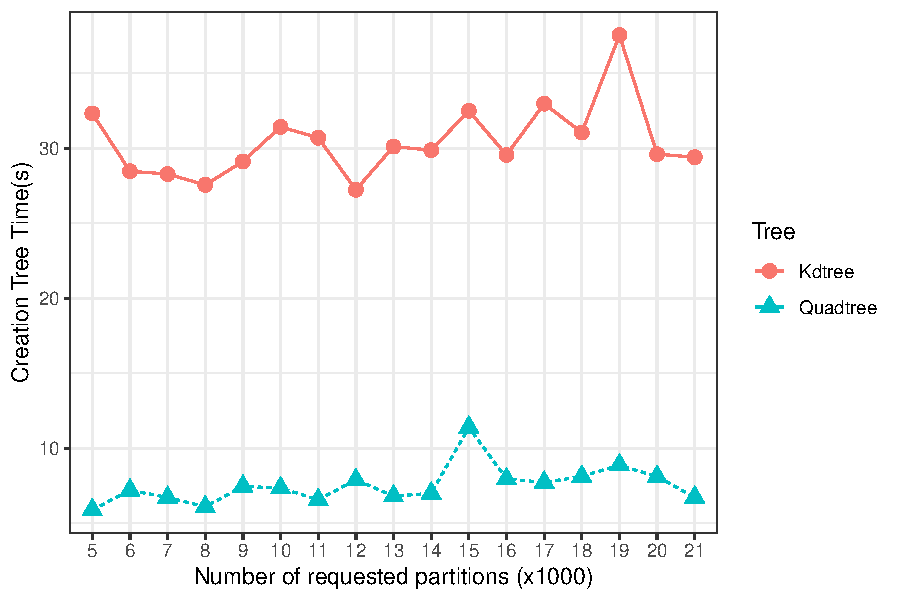
\includegraphics[width=0.49\linewidth]{chapterSDCEL/K_Creation_GADM.pdf} \\
%         (a) & (b)
%     \end{tabular}
%     \caption{Construction time for the spatial data structure in the (a) MainUS and (b) GADM datasets.} \label{fig:k_creation_us}
% \end{figure}

% \begin{figure}
%     \centering
%     \begin{tabular}{cc}
%         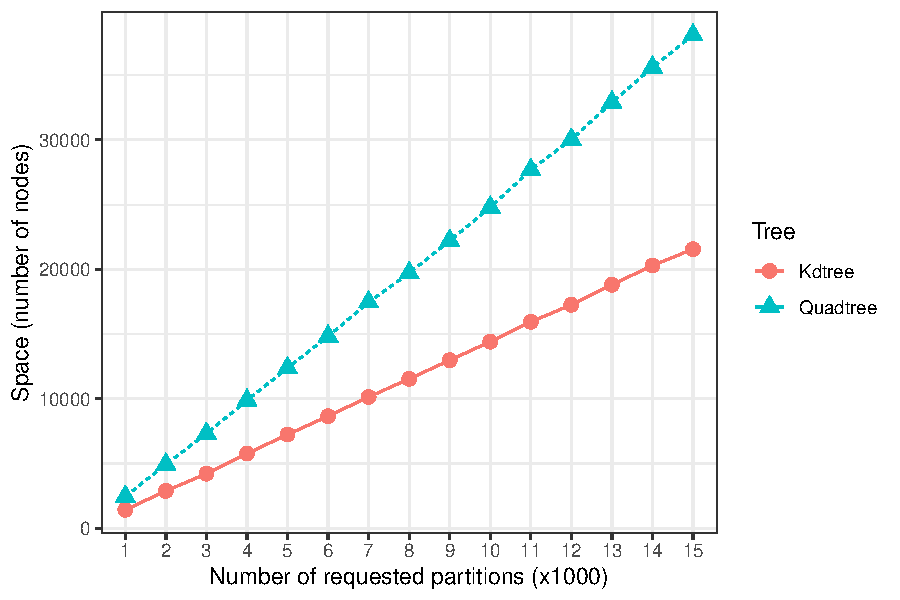
\includegraphics[width=0.49\linewidth]{chapterSDCEL/K_Space_US.pdf} & 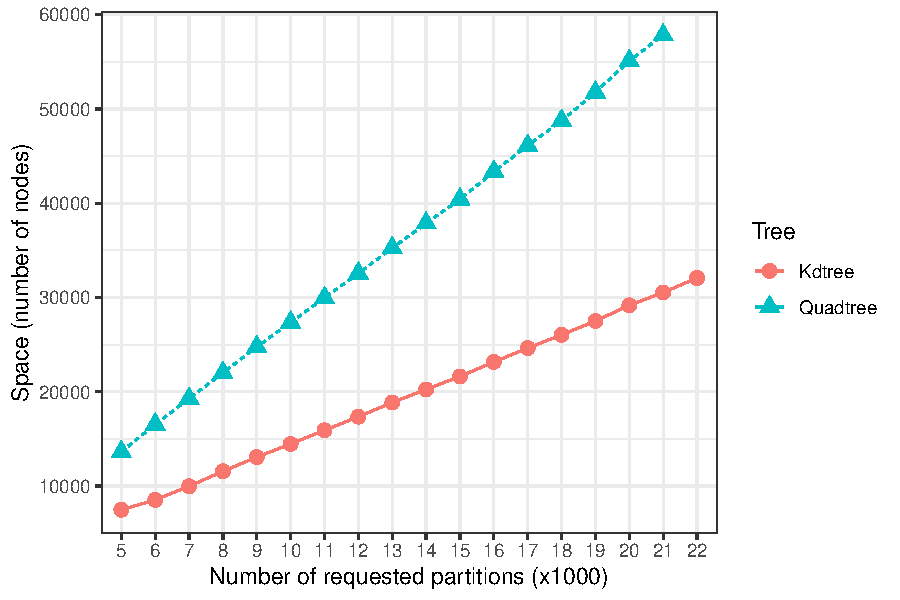
\includegraphics[width=0.49\linewidth]{chapterSDCEL/K_Space_GADM.pdf} \\
%         (a) & (b)
%     \end{tabular}
%     \caption{Number of cells created by each spatial data structure in the (a) MainUS and (b) GADM datasets.} \label{fig:k_space_us}
% \end{figure}

% Figure \ref{fig:k_creation_us} depicts the construction time during the sampling of the input layers and the generation of the partitioning cells after requesting a different number of divisions. We can see that the kd-tree takes more time, particularly because of the sorting done at each split, so as to organize the data and localize the middle point. In average, Quadtree takes 23.13\% the time it takes for Kdtree to be created (21.55\% in MainUS and 24.72\% in GADM). However, the Kdtree creation is just 5.86\% of the overall time during the total DCEL construction (6.88\% in MainUS and 4.87\% in GADM).

% \begin{figure}
%     \centering
%     \begin{tabular}{cc}
%         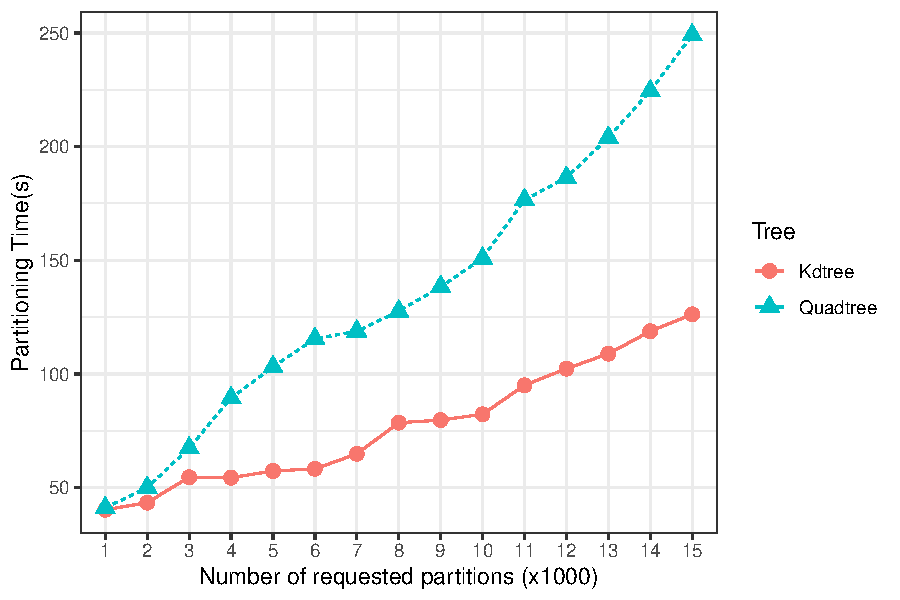
\includegraphics[width=0.49\linewidth]{chapterSDCEL/K_Partitioning_US.pdf} &
%         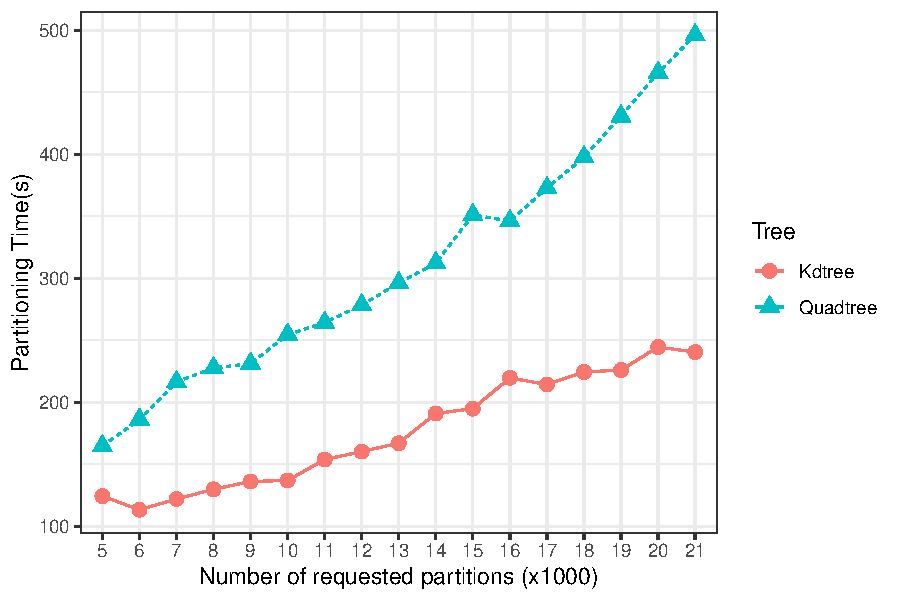
\includegraphics[width=0.49\linewidth]{chapterSDCEL/K_Partitioning_GADM.pdf} \\
%         (a) & (b)
%     \end{tabular}
%     \caption{Data partitioning time using a spatial data structure (a) in the MainUS dataset and (b) in the GADM dataset.} \label{fig:k_partitioning_us}
% \end{figure}

%An important characteristic of the behavior of each partitioning scheme is the number of cells (partitions) each sample data structure creates. Figure \ref{fig:k_space_us} depicts the number of cells created by each spatial data structure. As the quadtree follows a space-oriented technique, it creates more nodes (4 at each split) and thus generates more leaves (cells); more of them are prone to be empty compared to the kd-tree.

%Figure \ref{fig:k_partitioning_us} shows the cost to partition the full content of both layers. Given a sample tree data structure, each edge is assigned to a cell (partition) depending on which leaf the edge is located; edges are assigned (copied) to all leaves they intersect. Then, a shuffle operation is performed to move the data to the corresponding node that will handle this cell (partition). This figure shows that the quadtree partitioning takes more time. This depends largely on the number of leaves created by the sample tree and the number of edges that overlap partitions (which is expected to be larger for the quadtree since it uses more and thus smaller cells).

% \begin{figure}
%     \centering
%     \begin{tabular}{cc}
%         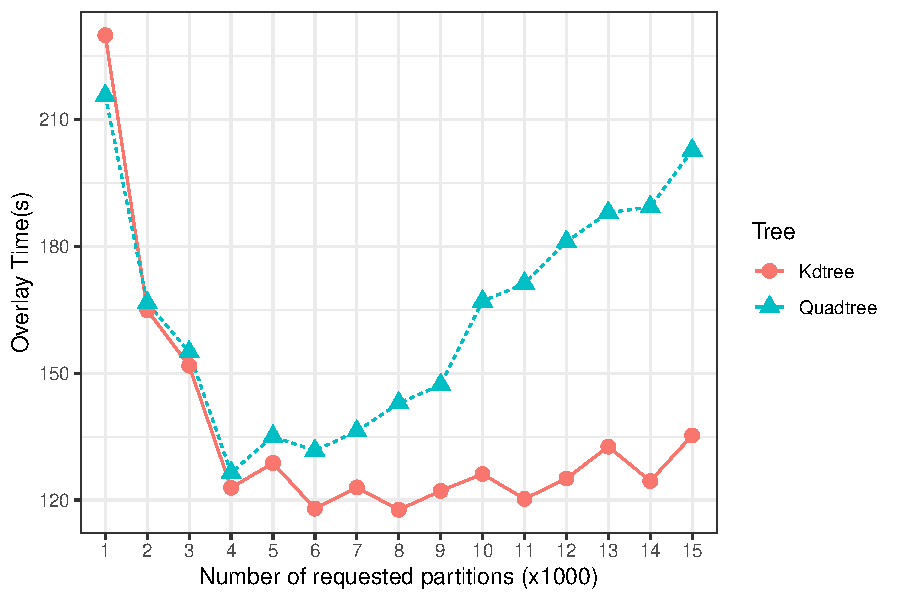
\includegraphics[width=0.49\linewidth]{chapterSDCEL/K_Overlay_US.pdf} &
%         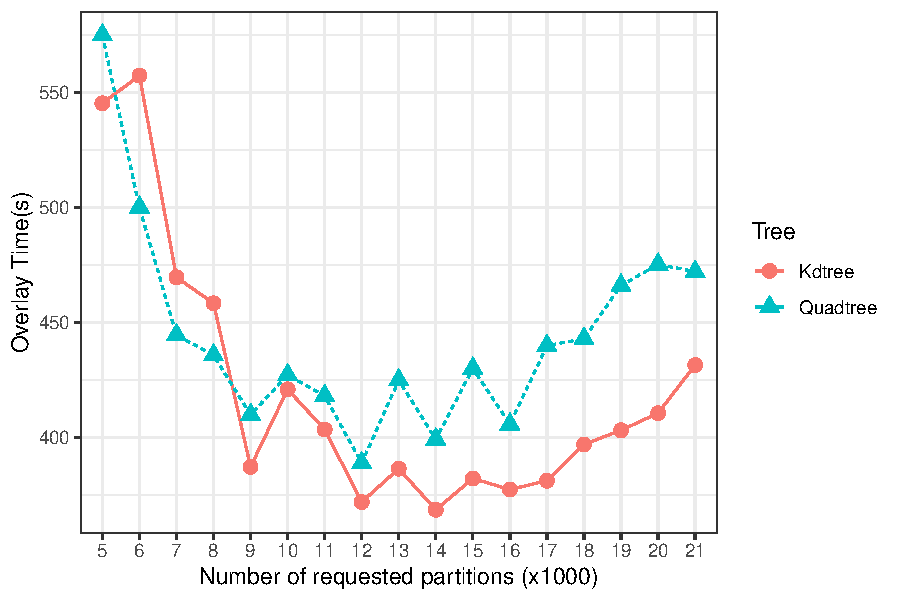
\includegraphics[width=0.49\linewidth]{chapterSDCEL/K_Overlay_GADM.pdf} \\
%         (a) & (b)
%     \end{tabular}
%     \caption{Execution time for the overlay operation using a spatial data structure in the MainUS (a)and GADM (b) dataset.} \label{fig:k_overlay_us}
% \end{figure}

%Once the data is assigned to their partitions, the overlay operation can be executed.  Figure \ref{fig:k_overlay_us} shows the overlay performance under each partition strategy, for different number of cells. The Kd-tree approach performs better; as the quadtree tends to generate more and emptier cells, its performance is directly affected.

%As it was said before, in particular on partitioning based on Kdtree, the smaller number of cells/partitions used in this approach give also an improvement on the impact of shuffling during the partition strategy because the number and size of the resulting partitions have a lower impact into the communication cost.

%Finally, we consider the speed-up and scale-up performance using the kd-tree partitioning. Figure \ref{fig:k_scale_speed_us}(a) shows the speed-up performance using the MainUS dataset (36M edges) while varying the number of nodes (for 3, 6, and 12 nodes). Similar to the quadtree partitioning strategy, the kd-tree partitioning shows good speed-up performance. As resources duplicate the execution time improves almost by a half.

%Figure \ref{fig:k_scale_speed_us}(b) shows the scale-up performance of the kd-tree partitioning approach. We followed the same procedure described in Section \ref{sec:speed_scale} to generate datasets for 8M, 16M, and 32M edges from the MainUS dataset and ran the kd-tree partitioning strategy with 3, 6, and 12 nodes, respectively. Again the kd-tree partitioning shows good speed-up performance, which remains flat as the load per node is almost equal.

% \begin{figure}
%     \centering
%     \begin{tabular}{cc}
%         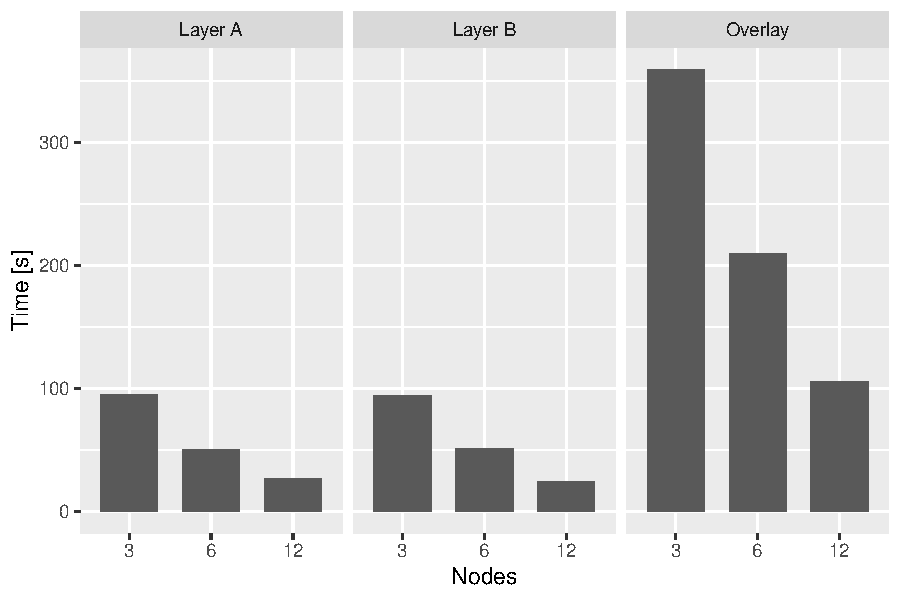
\includegraphics[width=0.49\linewidth]{chapterSDCEL/US_speedup.pdf} & 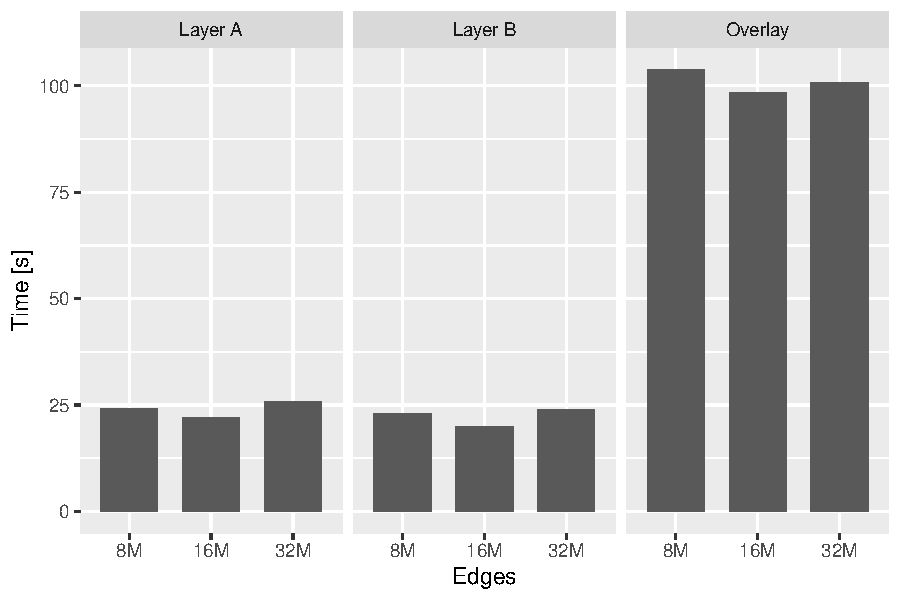
\includegraphics[width=0.49\linewidth]{chapterSDCEL/US_scaleup.pdf} \\
%         (a) & (b)
%     \end{tabular}
%     \caption{(a)Speed Up and (b) Scale Up performance of the Kdtree partitioning using the MainUS dataset.} \label{fig:k_scale_speed_us}
% \end{figure}


%% Extension
%\subsection{Polygonization Scalability}\label{sec:expr:query}
% \begin{table}
%     \centering
%     \caption{Polygonization Evaluation Dataset}
%     \label{table:polygonization:datasets}
%     \begin{tabular}{c c c c c}
%         \toprule
%         Dataset  & Area & Number of Line Segments & Faces \\
%         \midrule
%         USA & 9.83 $Mkm^2$ & 152$M$ & 5$M$ \\
%         South America & 17.8 $Mkm^2$ & 155$M$ & 7$M$\\
%         North America & 24.7 $Mkm^2$ & 240$M$ & 10$M$ \\
%         Africa & 30.4 $Mkm^2$ & 288$M$ & 10$M$  \\
%         Europe & 10.2 $Mkm^2$ & 563$M$ & 25$M$ \\
%         Asia & 44.6 $Mkm^2$ & 557$M$ & 23$M$ \\
%         \bottomrule
%     \end{tabular}
% \end{table}

% \begin{figure}
% \centering
% 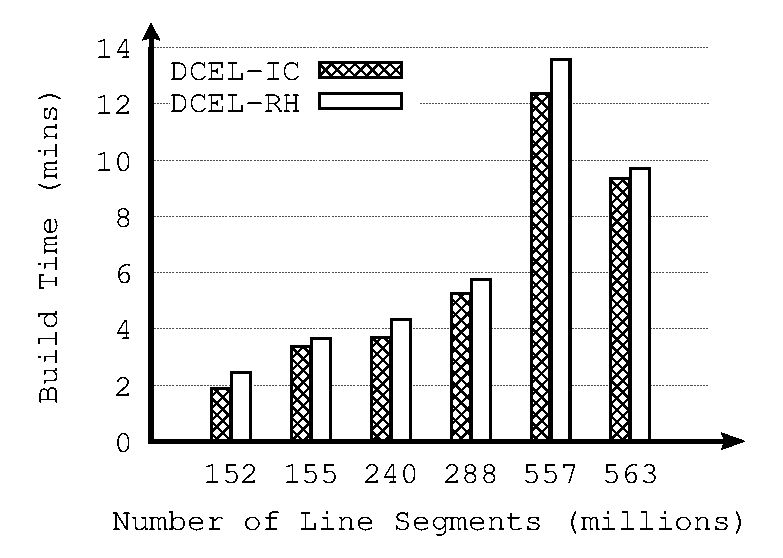
\includegraphics[width=0.48\linewidth]{chapterSDCEL/Experiments/n_records.eps}
% 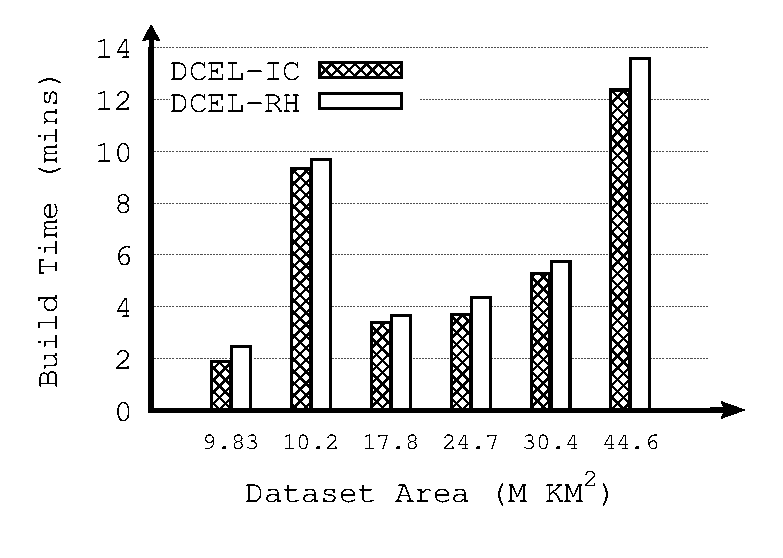
\includegraphics[width=0.48\linewidth]{chapterSDCEL/Experiments/area.eps}
% \caption{Polygonization Performance on Real Road Networks.}
% \label{fig:exp:query}
% \end{figure}

%Figure \ref{fig:exp:query} evaluates the scalability of the polygonization approach using the different evaluation datasets summarized in Table \ref{table:polygonization:datasets}.  We implemented our polygonization framework on Apache Sedona \cite{yu_spatial_2018}. The experiment is based on a Java 8  implementation and utilizes a Spark 2.3 cluster with two driver nodes and 12 worker nodes. All nodes run Linux CentOS 8.2 (64-bit). Each driver node is equipped with 128GB of RAM, while each worker node has 64GB of RAM. To increase parallelism, we divided the 12 worker nodes into 84 worker executors. Each executor is a separate JVM process with dedicated resources, such as memory and CPU cores. The distribution of these executors across the nodes is managed by the resource negotiator (YARN), which allocates resources for Spark jobs based on the availability of cores and memory. YARN typically balances resources across the cluster, so executors are likely to be evenly distributed, though some variation may occur due to resource availability at runtime. Assuming an even distribution, each worker node would run approximately 7 executors, as calculated by $\frac{84}{12} = 7$.

%As discussed in Section \ref{sec:rem}, the Rem Phase has two different approaches depending on the input data received from the Gen Phase. The first approach is to process the remaining half-edges iteratively, denoted as \textit{DCEL-RH}. In comparison, the second approach processes the incomplete cycles generated from the first phase iteratively denoted as \textit{DCEL-IC}.

%From Figure \ref{fig:exp:query}, we draw three conclusions; (1) first, the cardinality of the input dataset has a positive correlation with the build time; as the number of line segments increases, the build time also increases, as shown in Figure \ref{fig:exp:query}(a). However, we see that we have close cardinality for Asia (557M) and Europe (563M) datasets, but there is a noticeable difference in the build time; moreover, the build time for the Europe dataset is less than that of the Asia dataset. This drives us to the second conclusion; (2) for datasets with close or similar cardinalities, the area of the dataset has a positive correlation with the build time shown in Figure \ref{fig:exp:query}(b). Hence the build time of the Europe dataset (10.2 $Mkm^2$) is less than that of the Asia dataset (44.6 $Mkm^2$), even though Europe has a slightly larger dataset.  (3) The third conclusion is that for all evaluated datasets, the \textit{DCEL-IC} beats \textit{DCEL-RH}.


%% Extension
%\subsection{Polygonization Speed Up Evaluation} \label{sec:expr:speedup}
% \begin{figure}[tb]
% 	\centering
% 	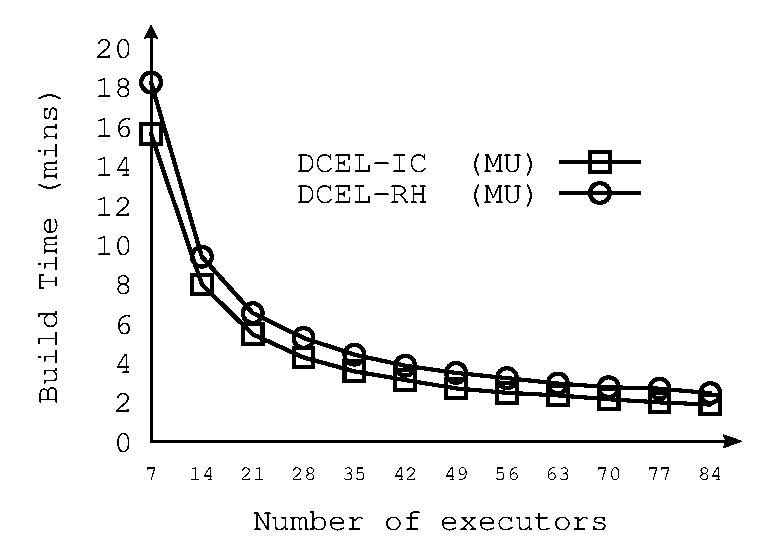
\includegraphics[width=8.8cm]{chapterSDCEL/Experiments/speedup.eps}
% 	\caption{Polygonization speed up evaluation using the USA dataset}
% 	\label{fig:exp:speedup}
% \end{figure}

%Figure \ref{fig:exp:speedup} shows the effect of increasing the number of executors on the build time for the USA dataset.  At each step in the figure, we add 7 more executors, which is approximately equivalent to adding one additional node.  Overall, our approach has good speedup performance. As the number of executors is doubled from 7 executors to 14 executors, the build time is almost halved.  This trend goes on as we double the number of executors. As we increase the number of executors from 7 to 84, the build time is decreased by a factor of 8.


%% Extension
%\subsection{Overlaying Polygons with Dangle and Cut Edges}
% \begin{table}
%     \caption{Overlaying Polygons with Dangle and Cut Edges Dataset}
%     \label{tab:dangles}
%     \begin{tabular}{c c c c}
%         \toprule
%         Dataset & Number Layer $A$ of Polygons & Number of Layer $B$ Edges & Result Polygons \\
%         \midrule
%         TN & 1,272 & 3,380,780 & 41,761 \\
%         GA & 1,633 & 4,647,171 & 49,125 \\
%         NC & 1,272 & 7,212,604 & 22,413 \\
%         TX & 4,399  & 8,682,950 & 98,635 \\
%         VA & 1,554 & 8,977,361 & 38,941 \\
%         CA & 7,038 & 9,103,610 & 96,916\\
%         \bottomrule
%     \end{tabular}
% \end{table}

% \begin{figure}
%     \centering
%     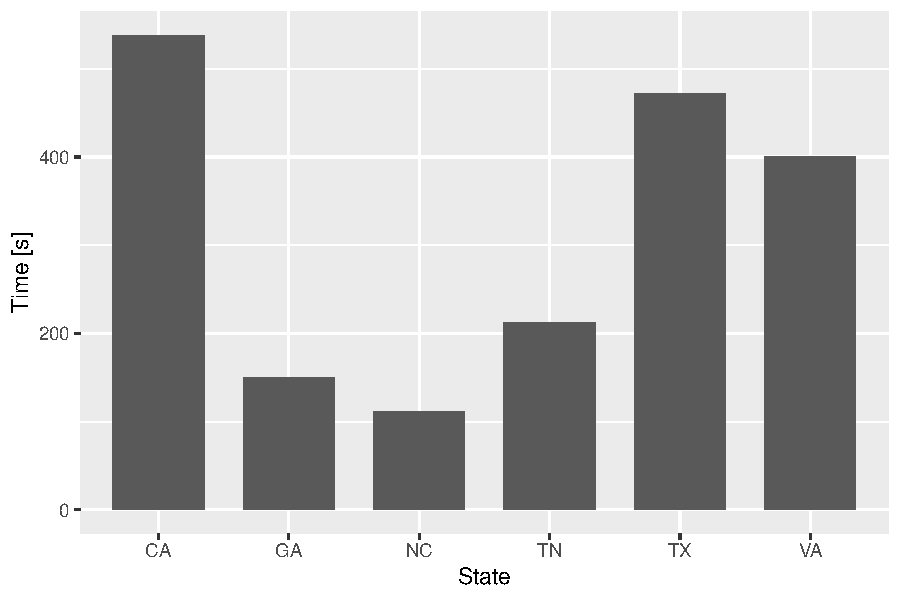
\includegraphics[width=0.7\linewidth]{chapterSDCEL/states.pdf}
%     \caption{Overlaying State polygons with dangle and cut edges.}
%     \label{fig:dangle}
% \end{figure}

%In this section, we examine the performance of overlaying polygons with dangle and cut edges resulting from the polygonization as detailed in Section \ref{sec:over_dang}.  Table \ref{tab:dangles} shows the number of polygons for each state for the first layer of the overlay. It also shows the number of dangle and cut edges per state for the second layer of the overlay. Finally, it shows the number of resultant polygons per state.  From Figure \ref{fig:dangle}, we conclude that the running time is affected by the number of dangle and cut edges and the number of intersections between the two layers (represented by the number of generated polygons).  TN and GA have a relatively smaller number of dangle and cut edges, so they have lower execution times compared to VA, TX, and CA. However, since the intersections in NC are significantly less than those of TN and GA, NC has the lowest execution time. TX, VA, and CA have a comparable number of edges; however, VA has the least number of intersections, resulting in lower execution time compared to TX and CA.

%\chapter{Conclusions}
We introduced SDCEL, a scalable approach to compute the overlay operation among two layers that represent polygons from a planar subdivision of a surface. Both 
input layers use the DCEL edge-list data structure to store their polygons. Existing sequential DCEL overlay implementations fail for large datasets. We first 
presented a partition strategy which guarantees that each partition collects the required data from each layer to work independently. 
We also proposed several optimizations to improve performance. Our experimental evaluation using real datasets shows that SDCEL has very good scale-up and 
speed-up performance and can compute the overlay over very large layers (up to 37M edges) in few seconds.


\chapter{Scaling DCEL Overlay Operations to Support Dangle and Cut Edges}

\section{Introduction} %\label{sec:extenstion_introduction}

This chapter extends the previous work in \cite{calderon_scalable_2023}. The main new contributions are summarized as follows. First, we introduce a new spatial partitioner, based on the kd-tree partitioning strategy, for constructing overlay  DCELs (section \ref{sec:pstrategies}). Since it better utilizes the data distributions in optimizing DCEL partitions, it leads to noticeably improved performance. The new partitioning strategy contrasts with the original strategy that employed space-partitioning techniques based on quadtrees. 

Second, we extend the overlay DCEL approach to accept scattered and noisy line segments as input, rather than being restricted to clean polygon data. This enhancement builds on the scalable polygonization methods presented in \cite{abdelhafeez_ddcel_2023}, enabling the overlay of real-world datasets composed of vast sets of line segments —datasets that existing techniques are unable to process effectively.

For instance, Figure \ref{fig:extension_dcel_example} illustrates the fundamental components of a DCEL. Additionally, we identify two types of special half-edges. \textit{Dangles} are half-edges with one or both endpoints not incident on another half-edge endpoint; both half-edge $\overrightarrow{fj}$ and its twin are considered dangle edges. \textit{Cut-edges} are half-edges connected at both ends that do not form part of any polygon. The half-edge $\overrightarrow{dg}$ and its twin are classified as cut-edges.

\begin{figure}
    \centering
    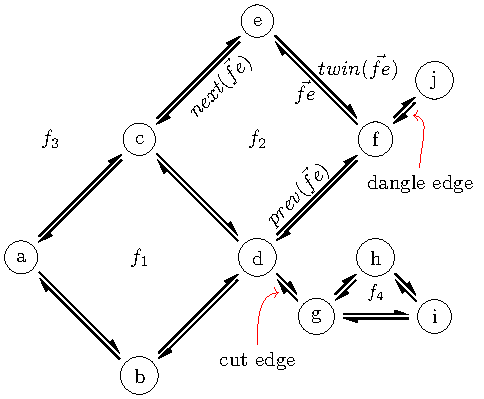
\includegraphics[width=0.6\linewidth]{chapterExtension/dcel_example2}
    \caption{Components of the DCEL structure with dangle and cut edges.}\label{fig:extension_dcel_example}
\end{figure}

The remainder of this chapter is organized as follows. Section \ref{sec:extension_methods} details the implementation of the new kd-tree partitioner and describes the polygon extraction process for adapting line segment inputs, which extends the overlay method to support dangle and cut edges. In Section \ref{sec:extension_experiments}, we present additional experiments to quantify the benefits of the kd-tree-based strategy and assess the performance of the proposed polygonization on datasets with large volumes of line segments.

\section{Scalable Kd-tree Partitioner with Dangle and Cut Edges Integration} \label{sec:extension_methods}

\subsubsection{Kd-tree Partition Strategy} %\label{sec:kdtreestrategy}
In Section \ref{sec:pstrategies}, we use the quadtree spatial index as the baseline for our partitioning strategy. The quadtree follows a space-oriented approach, as it does not consider the content of each cell when determining potential splits. In contrast, kd-tree-based partitioning employs a data-oriented approach by sorting and selecting the midpoint within a cell to guide the placement of splits for future child nodes.

Building and populating the kd-tree partitioning follows a process similar to that of the quadtree. First, a kd-tree is constructed from a sample representing 1\% of the input data to define the tree’s structure, where the leaves represent the partition’s cells. The input data is then fed into this kd-tree structure, with each edge assigned to the leaf cell containing its boundaries. After partitioning, the local DCELs for each layer are constructed, and the overlay operation is performed within each cell as described in Section \ref{sec:pstrategies}.

Section \ref{sec:extension_experiments} will compare two partitioning strategies, the one presented in \ref{sec:pstrategies} based on the quadtree (i.e. space-oriented) and one on the kd-tree (i.e. data-oriented) indexes.  Note that both tree-based data partitioning involves shuffling all edges; this however, happens only once. Our experimental evaluation (see Section \ref{sec:comparison}) shows that the data-oriented approach leads to better performance. 

\subsection{Overlaying Polygons with Dangle and Cut Edges} \label{sec:over_dang}

Beyond scalability challenges, many modern applications receive spatial polygon datasets as scattered line segments—for example, road segments that form city blocks. Such datasets can be extremely large and are common in fields like urban planning, geo-targeted advertising, economic and demographic studies, and more. However, existing polygon overlay techniques are not equipped to process them directly at scale. In this section, we extend the overlay method presented in Section \ref{sec:methods} to support polygonal input by integrating a scalable, distributed polygon extraction approach. This enhancement enables the merging of polygons with dangle and cut edges.

We built on in the scalable polygonization procedure presented in \cite{abdelhafeez_ddcel_2023}.  The result of that polygonization procedure generates two outputs: first, a set of closed polygons formed by the input planar line segments, and second, any edges that are not a part of any polygon (i.e., dangle or cut edges).  Overlaying the polygons generated with any polygon layer follows the approaches discussed in sections \ref{sec:methods} and \ref{sec:alternative_methods}.  However, we need to modify the algorithms provided in these previous sections to overlay an input polygon layer $A$ with the dangle and cut edges (layer $B$). In particular, we modify the reduce phase.

We build upon the scalable polygonization procedure presented in \cite{abdelhafeez_ddcel_2023} (see Figure \ref{fig:polygonization}), which produces two outputs: (1) a set of closed polygons formed from the input planar line segments, and (2) any edges that are not part of any polygon (i.e., dangle or cut edges). Overlaying these generated polygons with any polygon layer follows the methods discussed in Sections \ref{sec:methods} and \ref{sec:alternative_methods}. However, to overlay an input polygon layer $A$ with the dangle and cut edges (layer $B$), we modify the algorithms from these sections, particularly adjusting the reduce phase.

 \begin{figure}
     \centering
     \begin{tabular}{cc}
         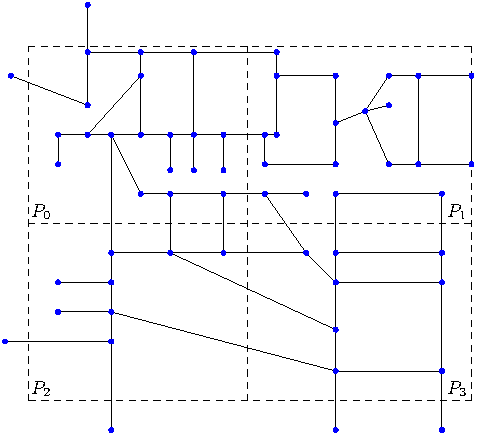
\includegraphics[width=0.49\textwidth]{chapterExtension/model/input/input} &
         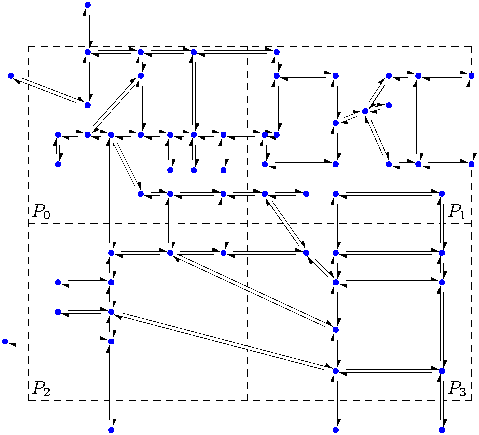
\includegraphics[width=0.49\textwidth]{chapterExtension/model/a/a} \\
         (a) & (b) \\
         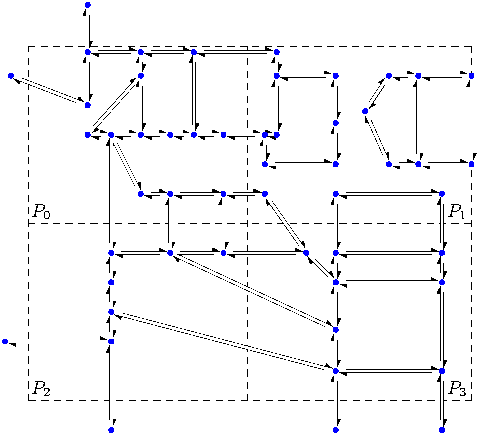
\includegraphics[width=0.49\textwidth]{chapterExtension/model/b/b} &
         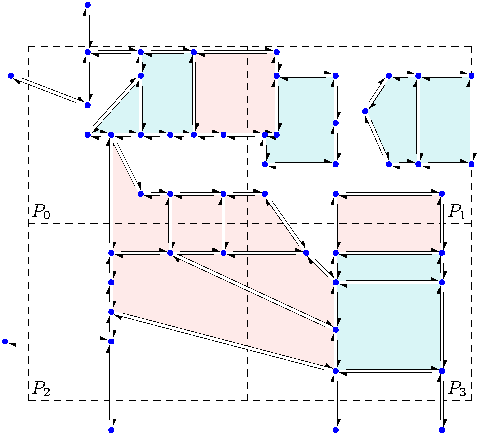
\includegraphics[width=0.49\textwidth]{chapterExtension/model/c/c} \\
         (c) & (d) \\
     \end{tabular}
     \caption{An example of four leaf nodes in a quadtree constructed for input spatial line segments. Solid lines represent the line segments, while dashed lines indicate the Minimum Bounding Rectangles (MBRs) of the partitions. (a) shows the partitioned input spatial lines. (b) shows the DCEL vertices and half-edges. (c) the resulting DCEL after  dangle and cut edge removal.  Finally, (d) shows the final DCEL faces. (taken from \cite{abdelhafeez_ddcel_2023}).} \label{fig:polygonization}
 \end{figure}

 \begin{figure}
    \centering
    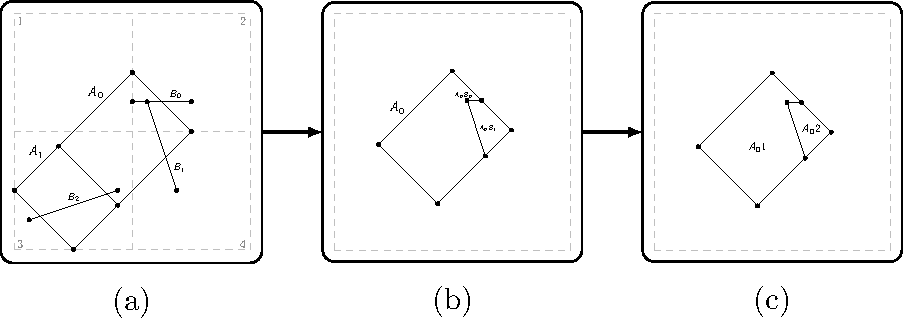
\includegraphics[width=\textwidth]{chapterExtension/dangles_cuts/DAC}
    \caption{(a) Spatial partitioning of input layers A and B, (b) Re-Partitioning of polygon $A_0$ with edges it intersects with, and (c) the result of polygonization of $A_0$ with $B_0, B_1, B_2$.} \label{fig:dangles_cuts}
 \end{figure}

 Figure \ref{fig:dangles_cuts}(a) illustrates the spatial partitioning of two input layers, $A$ and $B$. Layer $A$ contains two input polygons, $A_0$ and $A_1$, while Layer $B$ includes of three dangle edges, $B_0$, $B_1$, and $B_2$.
 
 Each edge in layer $B$ is assigned a unique label and provided as input to the overlay module.  The local overlay processs indentifies intersections between the input polygon layer $A$ and layer $B$ within each data partition.  If a polygon with $id = i$ from layer $A$ intersects with edges labeled $id = a$, $id = b$ and $id = c$ from layer $B$ in a given partition, a composite label $A_{i} B_{a} B_{b} B_{c}$ is generated to represent these intersections.  
 
During the reduce phase, we re-partition the data based on the first label, consolidating all edges that intersect with it. For instance, if two data partitions generate the labels $A_{i} B_{a} B_{b} B_{c}$ and $A_{i} B_{x} B_{y}$, we reassign the data so that $A_{i}$ is grouped within a single partition along with all intersecting edges, specifically $B_{a}, B_{b}, B_{c}, B_{x}, B_{y}$.  In Figure \ref{fig:dangles_cuts}(b), polygon $A_0$ is re-partitioned with the edges it intersects, namely $B_0$, $B_1$, and $B_2$.

After re-partitioning, all intersecting edges from both layers are consolidated within the same partition. The next step is to identify the polygons formed by these intersections. Since there is no guarantee that only one polygon will be generated, we replace the polygon concatenation method proposed in Section \ref{sec:optimizing} with a \textit{polygonization} procedure within each partition. This polygonization process ensures that all possible new polygons are generated.

The polygonization procedure follows the algorithm outlined in \cite{abdelhafeez_ddcel_2023}. It begins by generating new vertices and half-edges, marking the current dangle and cut edges, setting the next pointers, and finally constructing the partition polygons. Figure \ref{fig:dangles_cuts}(c) illustrates the result of polygonizing the edges from polygon$A_0$ and $B_0$, $B_1$, and $B_2$, yielding two polygons,$A_01$ and $A_02$.  The polygons generated from all partitions together form the overlay between polygon layer $A$ and layer $B$.

\section{Experimental Evaluation} \label{sec:extension_experiments}

\subsection{Overlaying Polygons with Dangle and Cut Edges}

\begin{table}
    \small
    \caption{Overlaying Polygons with Dangle and Cut Edges Dataset}
    \label{tab:dangles}
    \begin{tabular}{c c c c}
        \toprule
        Dataset & Number Layer $A$ of Polygons & Number of Layer $B$ Edges & Result Polygons \\
        \midrule
        TN & 1,272 & 3,380,780 & 41,761 \\
        GA & 1,633 & 4,647,171 & 49,125 \\
        NC & 1,272 & 7,212,604 & 22,413 \\
        TX & 4,399  & 8,682,950 & 98,635 \\
        VA & 1,554 & 8,977,361 & 38,941 \\
        CA & 7,038 & 9,103,610 & 96,916\\
        \bottomrule
    \end{tabular}
\end{table}

\begin{figure}
    \centering
    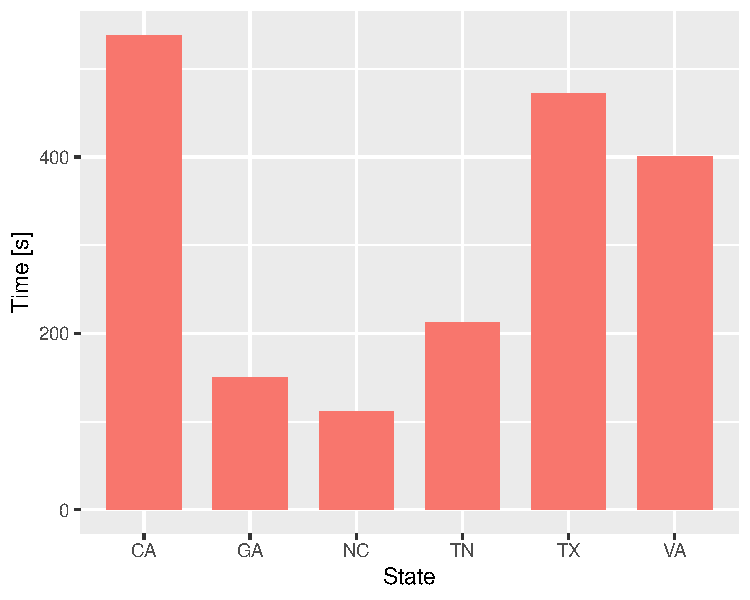
\includegraphics[width=0.75\textwidth]{chapterExtension/states.pdf}
    \caption{Overlaying State polygons with dangle and cut edges.}
    \label{fig:dangle}
\end{figure}

In this section, we examine the performance of overlaying polygons with dangle and cut edges resulting from the polygonization process, as detailed in \ref{sec:over_dang}.  Table \ref{tab:dangles} presents the number of polygons per state for the first overlay layer, the number of dangle and cut edges per state for the second overlay layer, and the number of resulting polygons per state.

From Figure \ref{fig:dangle}shows that the running time is influenced by both the number of dangle and cut edges and the number of intersections between the two layers (indicated by the number of generated polygons). TN and GA have relatively fewer dangle and cut edges, leading to lower execution times compared to VA, TX, and CA. However, because NC has significantly fewer intersections than TN and GA, it exhibits the lowest execution time overall. While TX, VA, and CA have a comparable number of edges, VA’s lower number of intersections results in a shorter execution time compared to TX and CA.


\chapter{Scalable Processing of Moving Flock Patterns}

\section{Introduction}
Technological advances in the past few decades have triggered an explosion in the collection of spatio-temporal data.  The increasing popularity of GPS devices and smartphones, along with the emergence of new disciplines such as the Internet of Things (IoT) and high-resolution Satellite/UAS imagery, has made it possible to collect vast amounts of data with spatial and temporal components.

In tandem, interest in extracting valuable information from such large databases has also grown.  Spatio-temporal queries about popular places or frequent events remain useful, but there has been growing interest in more complex patterns.  In particular, patterns that describe the group behavior of moving objects over significant periods.  Moving cluster \cite{kalnis_discovering_2005}, convoys \cite{jeung_discovery_2008}, flocks \cite{gudmundsson_computing_2006} and swarm patterns \cite{li_swarm_2010} reveal how entities move together over a minimum time interval.

Applications for this type of information are both diverse and intriguing, particularly when dealing with trajectory datasets \cite{jeung_trajectory_2011, huang_mining_2015}. Case studies span various domains, including transportation system management and urban planning \cite{di_lorenzo_allaboard_2016}, as well as ecology \cite{la_sorte_convergence_2016}. For example, \cite{turdukulov_visual_2014} explores the identification of complex motion patterns to discover similarities in tropical cyclone paths. Similarly, \cite{amor_persistence_2016} investigates eye movement trajectories to understand the strategies people use during visual searches. Additionally, \cite{holland_movements_1999} tracks the behavior of tiger sharks along the coasts of Hawaii to gain insight into their migration patterns.

One particular pattern of interest is the moving flock pattern, which captures how objects move within close proximity for a given time period. Closeness is defined by a disk of a specified radius within which the entities must remain. Since this disk can be positioned anywhere, detecting such patterns is a non-trivial problem. In fact, \cite{gudmundsson_computing_2006} highlights that finding flock patterns where the same entities stay together over time is an NP-hard problem. To address this, \cite{vieira_2009} proposed the BFE algorithm, the first approach capable of detecting flock patterns in polynomial time.

Despite the increasing availability of data, current state-of-the-art techniques for mining complex movement patterns still struggle with the performance demands of large-scale spatial data. This work introduces a scalable approach designed to detect moving flock patterns in very large trajectory databases. By leveraging emerging trends in distributed frameworks for spatial operations we aim to significantly improve the speed and efficiency of detecting these patterns.

\section{Related work}
The recent increased use of location-aware devices (such as GPS, smartphones, and RFID tags) has enabled the collection of vast amounts of data with spatial and temporal components.  Several studies have focused on discovering and analyzing these types of datasets \cite{leung_knowledge_2010, miller_geographic_2001}.  In this area, trajectory datasets have emerged as an interesting field where diverse kind of patterns can be identified \cite{zheng_computing_2011, vieira_spatio-temporal_2013}.  For instance, researchers have proposed techniques to discover spatial motion patterns such as moving clusters \cite{kalnis_discovering_2005}, convoys \cite{jeung_discovery_2008} and flocks \cite{benkert_reporting_2008, gudmundsson_computing_2006}.  Specifically, \cite{vieira_2009} introduced BFE (Basic Flock Evaluation), an innovative algorithm designed to efficiently identify moving flock patterns in polynomial time across large spatio-temporal datasets.

A flock pattern is defined as a group of entities that move together over a specified time period \cite{benkert_reporting_2008}. The applications of such patterns are broad and diverse. For instance, \cite{calderon_romero_mining_2011} identifies moving flock patterns in iceberg trajectories to analyze their movement behavior and their relationship with changes in ocean currents.

The BFE algorithm provides an initial approach for detecting flock patterns. It begins by identifying disks with a predefined diameter ($\varepsilon$) where moving entities are sufficiently close at specific time instants. This operation is computationally expensive due to the large number of points and time instances to be analyzed, with a complexity of $\mathcal{O}(2n^2)$ per time. Although the algorithm leverages a grid-based index and a stencil to accelerate this process, the overall complexity remains high.

Both \cite{calderon_romero_mining_2011} and \cite{turdukulov_visual_2014} adopt a frequent pattern mining approach to enhance performance when combining disks across time instants. Similarly, \cite{tanaka_improved_2016} utilize plane sweeping techniques, binary signatures, and inverted indexes to further accelerate this process. However, these methods retain the core strategy of BFE for detecting disks at each time instant.

In contrast, \cite{arimura_finding_2014} and \cite{geng_enumeration_2014} employ depth-first algorithms to analyze the time intervals of individual trajectories and report maximal duration flocks. However, these methods are less effective for dense datasets or those that involve large numbers of entities per time step, as they struggle to scale efficiently in such conditions.

Given the high computational demands of flock pattern detection, it is not surprising that parallelism has been employed to improve performance. For example, \cite{fort_parallel_2014} use extreme and intersection sets to report maximal, longest, and largest flocks on GPUs, albeit with limitations imposed by the GPU's memory model.

Despite the increasing adoption of cluster computing frameworks, particularly those with spatial data capabilities \cite{eldawy_spatialhadoop_2014, yu_demonstration_2016, pellechia_geomesa_2015, xie_simba_2016}, significant advancements in this area remain limited. To the best of our knowledge, this work is the first to explore the detection of moving flock patterns in a scalable approach.

\section{Background}
%This section outlines an alternative methodology for identifying moving flock patterns in large spatio-temporal datasets, utilizing modern distributed frameworks to partition and parallelize the workload.  
Before discussing the details of our contributions, we first provide an overview of the current state-of-the-art. This will help highlighting their challenges and limitations in handling large spatio-temporal datasets, as described in the next Section.

\subsection{The BFE sequential algorithm}
The alternative approach we will discuss closely follows the steps outlined in \cite{vieira_2009}. In that work, the authors introduced the Basic Flock Evaluation (BFE) algorithm, designed to identify flock patterns in trajectory databases. While the full details of the algorithm can be found in the source, we will provide a general overview of the key aspects. It is important to note that the BFE algorithm operates in two phases: first, it identifies maximal disks at the current time step; second, it extends and reports previous flocks by combining them with the newly discovered disks.

The input for the BFE algorithm consists of a set of points, a minimum distance $\varepsilon$ (which defines the diameter of the disks where the moving entities must lie), a minimum number of entities $\mu$ per disk, and a minimum duration $\delta$, representing the required time units that entities must remain together to be considered a flock. Based on this input, Figure \ref{fig:MF_flowchart} illustrates the workflow of the process in four general steps. The primary goal of this phase is to identify a set of disks at each time step, enabling the combination with future disks to form flocks.

\begin{figure}
    \centering
    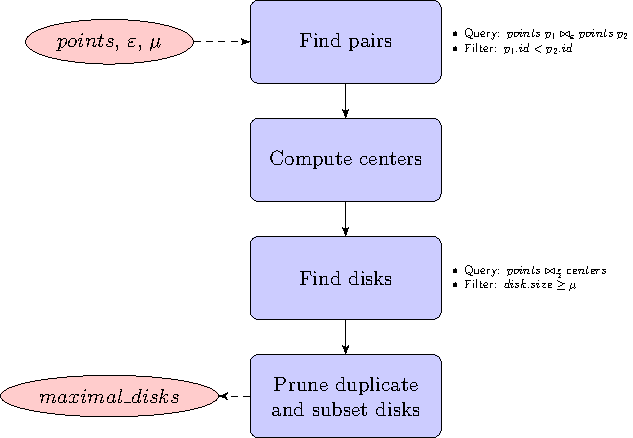
\includegraphics[width=0.85\linewidth]{chapterPFlocks/figures/MF_flowchart}
    \caption{General steps in phase 1 of the sequential algorithm.}\label{fig:MF_flowchart}
\end{figure}

The main steps in phase 1 follow:
\begin{enumerate}
    \item Pair finding:  The algorithm uses the parameter $\varepsilon$ to identify pairs of points that are within a maximum distance of $\varepsilon$ units 
from each other. This is achieved through a distance self-join operation on the set of points, using $\varepsilon$ as the distance threshold. To avoid 
redundancy, duplicate pairs are eliminated; for example, the pair $(p_1, p_2)$ is considered identical to the pair $(p_2, p_1)$, so only one instance is 
retained. Point IDs are used to filter out these duplicates efficiently.
    \item Center computation:  From the set of pairs obtained, each pair is used to compute the centers of two circles, each with a radius of 
$\frac{\varepsilon}{2}$, whose circumferences pass through the two points in the pair. The pseudo-code for this procedure is provided in Appendix 
\ref{app:centers}.
    \item Disk finding: Once the centers have been identified, a query is executed to gather the points within a distance of $\varepsilon$ units from each 
center. This is accomplished by performing a distance join between the set of points and the set of centers, using $\frac{\varepsilon}{2}$ as the distance 
parameter. As a result, each disk is defined by its center and the IDs of the surrounding points. At this stage, a filter is applied to discard any disks that 
contain fewer than $\mu$ entities.
    \item Disk pruning: It is possible for a disk to contain the same set, or a subset, of points as another disk. In such cases, the algorithm reports only 
that one disk which contains the other(s), referred to as the \textit{maximal} disk. The procedure for identifying maximal disks is explained in Appendix 
\ref{app:disks}.
\end{enumerate}

It is important to note that BFE also employs a grid structure in this phase to optimize spatial operations. The algorithm divides the space into a grid, where 
each cell has a side length of $\varepsilon$ (see Figure \ref{fig:grid} from \cite{vieira_2009}). This structure allows BFE to limit its processing to each grid 
cell and its eight neighboring cells. There is no need to query cells beyond this neighborhood, as points in more distant cells are too far away to influence 
the results. Figure \ref{fig:MF_stages} shows an example of the Phase 1 steps using a sample dataset.

\begin{figure}
    \centering
    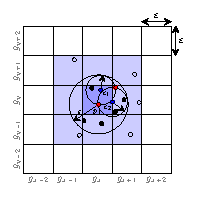
\includegraphics[width=0.5\linewidth]{chapterPFlocks/figures/grid_prime}
    \caption{The grid-based structure proposed in \cite{vieira_2009}.}\label{fig:grid}
\end{figure}

\begin{figure}
    \centering
    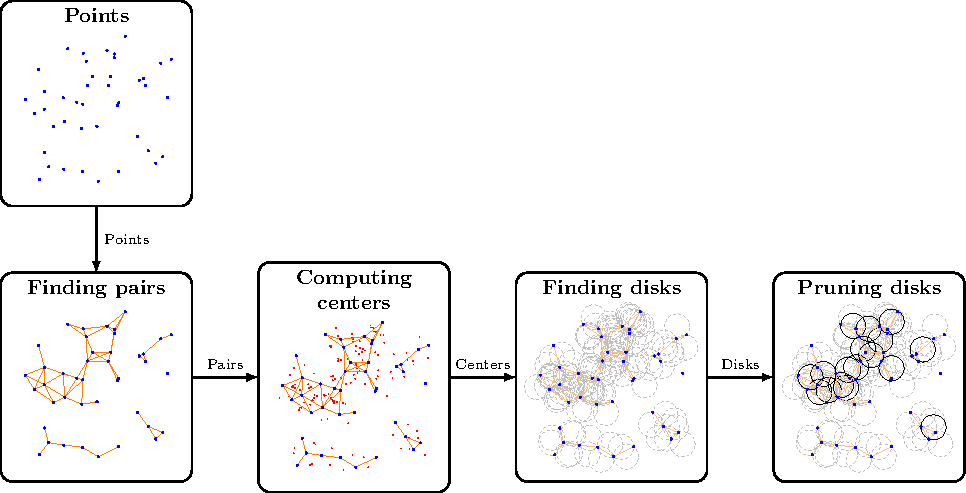
\includegraphics[width=\linewidth]{chapterPFlocks/figures/MF_stages2/flow}
    \caption{BFE Phase 1 example execution on a sample dataset.}\label{fig:MF_stages}
\end{figure}

Figure \ref{fig:FF_flowchart} explains schematically phase 2. This phase performs a recursion using the set of disks found at time $i$ and the set of partial 
flocks computed at the  previous time instant $i-1$.  As we do not know where and how far a group of points can move in the next time instant, this step 
performs a (temporal) join between both sets (partial flocks computed at time $i-1$ and maximal disks found in time $i$).  When a join is performed, we check 
that the number of common points remains greater than $\mu$, in which case the partial flock extends in time. A flock is reported in the answer if its duration 
has reached the minimum duration $\delta$; otherwise, it remains as partial flock and it will be further evaluated during the next iteration at the next time 
instant.

\begin{figure}
    \centering
    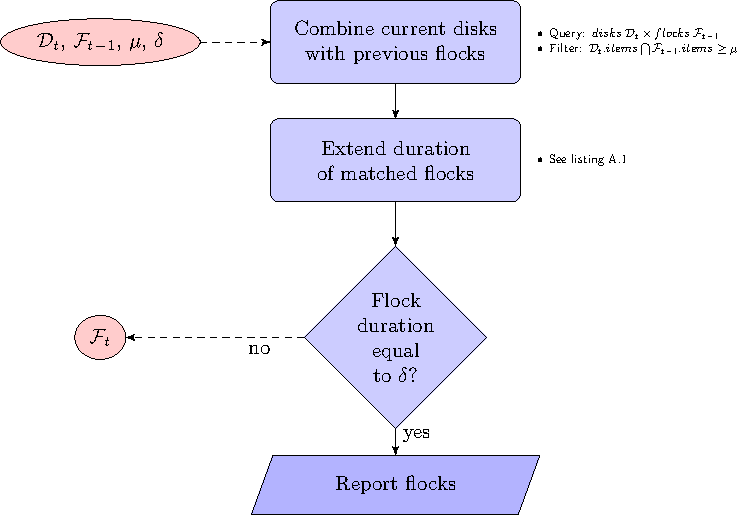
\includegraphics[width=0.85\linewidth]{chapterPFlocks/figures/FF_flowchart}
    \caption{Steps in BFE phase two. Combination, extension and reporting of flocks.}\label{fig:FF_flowchart}
\end{figure}

Similarly, Figure \ref{fig:FF_stages} illustrates the recursive process and how the set of partial flocks from previous time instants feeds into the next 
iteration. The example assumes a $\delta$ value of 3, meaning flocks start being reported from time instant $t_2$. Note that time instants $t_0$ and $t_1$ are 
considered the initial conditions. At the start of the algorithm, maximal disks are identified at $t_0$, which are immediately transformed into partial flocks 
with a duration of 1 and then passed on to the next time instant. At $t_1$, a new set of maximal disks $\mathcal{D}_1$ is found and joined with the partial 
flocks from $t_0$, denoted as $\mathcal{F}_0$. The information for each partial flock is updated accordingly, including its duration and the points it contains. 
From this point onward, subsequent time instants follow the exact steps outlined in Figure \ref{fig:FF_flowchart}.

\begin{figure}
    \centering
    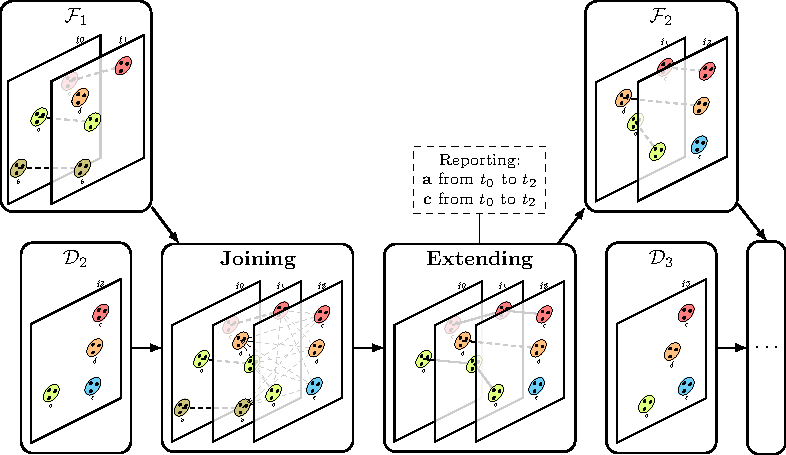
\includegraphics[width=\linewidth]{chapterPFlocks/figures/Temporal/f_stages}
    \caption{BFE Phase 2 example explaining the stages along time instants and the initial conditions.}\label{fig:FF_stages}
\end{figure}

\subsection{The PSI sequential algorithm}
The PSI algorithm, proposed by \cite{tanaka_improved_2016}, follows a similar process to the BFE algorithm. However, instead of using a grid structure to index 
points within the area, PSI employs a sweep-line approach that processes points in order of their x-coordinates. For each visited point $p$, the algorithm 
considers a square of side length $2\varepsilon$ centered at $p$. It only examines the points to the right of $p$ that lie within two half-squares of side 
length $\varepsilon$, as illustrated by the shaded regions in Figure \ref{fig:square}. 

While BFE processes points inside a grid cell of side length $\varepsilon$ along with its eight neighboring cells, PSI focuses on the points in these two 
half-squares. As a result, PSI more efficiently identifies the points relevant for detecting candidate pairs, centers, and disks. This indexing method has been 
shown to outperform BFE in most cases, with BFE offering similar or better performance only when $\varepsilon$ values are relatively small. In such cases, the 
number of points to consider is smaller, and PSI still requires sorting the points for the sweep-line approach. Therefore, both approaches are considered in the 
following sections.

\begin{figure}
    \centering
    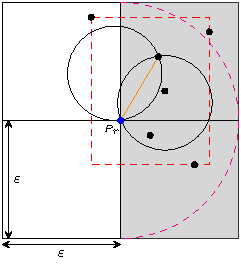
\includegraphics[width=0.45\linewidth]{chapterPFlocks/figures/square.pdf}
    \caption{An example of the two half squares used in PSI algorithm.}\label{fig:square}
\end{figure}

\section{Bottlenecks in the sequential approach and proposed solutions} %\label{spatial_phase}
Since both sequential approaches follow the same steps (as shown in Figures \ref{fig:MF_flowchart} and \ref{fig:FF_flowchart}), we will focus on discussing 
their bottlenecks using the BFE as an example. Certain stages in the BFE process are notably impacted when handling very large datasets, which can significantly 
affect performance.

\subsection{Phase 1: Spatial finding of maximal disks.}
First, we focus on Phase 1. As illustrated in Figure \ref{fig:MF_stages}, this phase's steps are demonstrated using a sample dataset. It is important to note 
that the final set of maximal disks is significantly smaller than the initial number of candidate disks found. Specifically, the number of candidate centers to 
evaluate is $2\lvert\tau\rvert^2$, where $\tau$ represents the number of trajectories \cite{vieira_2009}. Our experiments reveal that this issue becomes more 
pronounced not only in very large datasets but also in those containing areas with a high density of moving entities.

To address this issue, we propose a partition-based strategy that divides the study area into smaller subareas, allowing for independent and parallel 
evaluation. The strategy consists of three key steps: first, the \textit{partition and replication} stage, followed by the \textit{local flock discovery} within 
each partition, and finally, the \textit{filtering stage}, where we consolidate and unify the results. Each of these steps is detailed below.

\begin{itemize}
    \item Partition and Replication: Figure \ref{fig:partrep} provides a brief example of the partition and replication stage. Different types of spatial 
indexes, such as grids, R-trees, or quadtrees, can be used to create spatial partitions of the input dataset. In the example shown in Figure 
\ref{fig:partrep}.b, we use a quadtree, which generates seven partitions. To ensure each partition can locally identify flocks, it must have access to all 
relevant data. This is achieved by replicating points that are within a distance of $\varepsilon$ from the border of each partition, an area referred to as the 
\textit{expansion zone}, into adjacent partitions. Figure \ref{fig:partrep}.c illustrates each partition, surrounded by a dotted line representing the expansion 
zone, which includes the points that need to be replicated from neighboring partitions.

    \item Local flock discovery: At this stage, each partition can be processed independently and in parallel, with partitions assigned to different processing 
nodes. Within each partition, we can execute the steps of Phase 1 of the BFE algorithm locally, as outlined in Figure \ref{fig:MF_flowchart}.

    \item Filtering: While partitioning and replication facilitate parallelism, they can also lead to result duplication, as different nodes may report the same 
maximal disk. Specifically, if a disk's center lies within a partition, it will be reported only once by the node processing that partition. However, disks with 
centers located in an expansion zone will be reported by all partitions that share that zone. To address this, we propose a reporting approach that effectively 
prevents such duplication, which we detail below.
\end{itemize}

\begin{figure}
    \centering
    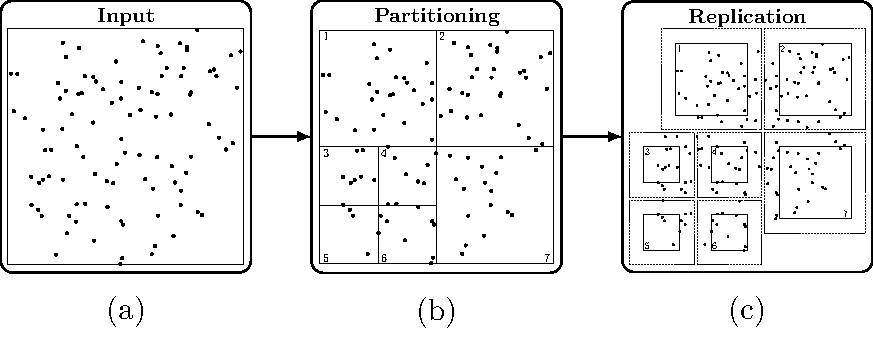
\includegraphics[width=\linewidth]{chapterPFlocks/figures/PartReplication/P123}
    \caption{An example of partitioning and replication on a sample dataset.}\label{fig:partrep}
\end{figure}

Disks with centers in an expansion zone are created by points that exist in both partitions due to replication. We assert that each partition should only report 
disks generated within its own area and not those originating in its expansion zone. Figure \ref{fig:ensuring} illustrates the possible scenarios. Assume 
partitions 1 and 2 in the figure are contiguous, sharing edge AB. Consider the disks $a^\prime$ and $a^{\prime\prime}$ (each with a diameter of $\varepsilon$), 
which are generated by two points (shown in green) located in the expansion zone of partition 1 but inside partition 2. In this case, both $a^\prime$ and 
$a^{\prime\prime}$ will be reported by partition 2. Similarly, both $c^\prime$ and $c^{\prime\prime}$ will be reported by partition 1. However, $b^\prime$ will 
be reported by partition 1, while $b^{\prime\prime}$ will be reported by partition 2.

\begin{figure}
    \centering
    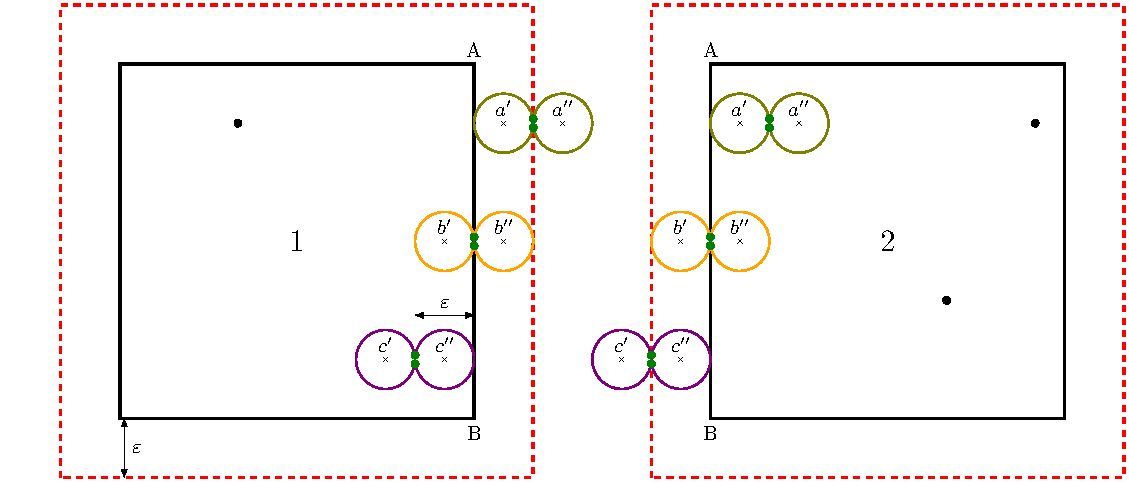
\includegraphics[width=\linewidth]{chapterPFlocks/figures/merge.pdf}
    \caption{Ensuring no loss of data in safe zone and expansion area.}\label{fig:ensuring}
\end{figure}

\subsection{Phase 2: Temporal join}\label{sec:temporal_join}
At the end of Phase 1, we have computed a set of maximal disks for a given time instant. In Phase 2, we proceed by combining these disks over time instants to 
form flocks. However, since Phase 1 involved partitioning the spatial domain for parallelism, Phase 2 becomes more complex as flocks can move across spatial 
partitions over time. Once the maximal disks are identified for a time instant $i$, a temporal join occurs within each partition to link these disks with 
partial flocks from the previous time instant ($i-1$). However, we must account for partial flocks that may appear near the partition borders and potentially 
move into adjacent partitions.

\begin{figure}
    \centering
    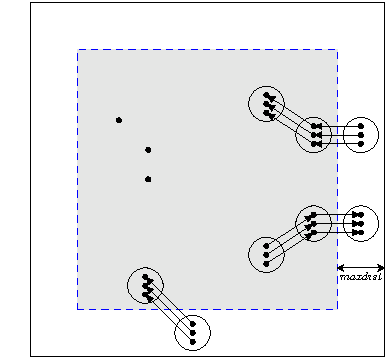
\includegraphics[width=0.5\linewidth]{chapterPFlocks/figures/maxdist.pdf}
    \caption{Examples of CPFs that that start or end in the border area of a partition.}\label{fig:maxdist}
\end{figure}

To address this issue, we introduce an additional parameter, \textit{maxdist}, which represents the maximum distance a moving object can travel between 
consecutive time instants (see Figure \ref{fig:maxdist}). We define the \textit{safe area} of a partition as the internal region that is at least \textit{maxdist} away from the partition’s border (illustrated in grey in Figure \ref{fig:maxdist}). Any partial or full flocks discovered within a partition’s safe area can be directly reported as results. However, flocks that start or end outside the safe area must be collected for post-processing to determine if they correspond with partial flocks from neighboring partitions. These cases, where flocks cross between partitions, are referred to as \textit{crossing partial flocks} (CPFs).  

In Figure \ref{fig:simple_alternative} we can see an example of the possible cases.  It shows flocks $a$ and $d$ which happen inside of the safe area of the orange partition, both of them are ready to be reported.  However, flocks $a$ and $c$ travel along different partitions.  Flock $a$ starts in $t_0$ in partition blue and move to partition orange in $t_2$.  It will create 2 CPFs: $a^{\prime}$ from $t_{0}$ to $t_{1}$ reported by the orange partition and $a^{\prime \prime}$ from $t_{2}$ to $t_{4}$ reported by the blue partition.  Similarly, flock $c$ starts in $t_0$ in partition blue and move to partition orange in $t_2$, then it come back to partition blue in $t_3$.  It will create 3 CPFs: $c^{\prime}$ from $t_{0}$ to $t_{1}$ reported by the blue partition, $c^{\prime \prime}$ in ${t_2}$ reported by the orange partition, and $c^{\prime \prime \prime}$ from $t_{3}$ to $t_{4}$ reported by the blue partition.

In Figure \ref{fig:simple_alternative}, we observe an example illustrating the possible cases. The figure shows flocks $a$ and $d$, which occur within the safe area of the orange partition; both of these flocks are ready to be reported. However, flocks $a$ and $c$ move across different partitions. 

Flock $a$ begins in partition blue at $t_0$ and moves to partition orange at $t_2$. This movement results in two CPFs: $a^{\prime}$, from $t_{0}$ to $t_{1}$, reported by the orange partition, and $a^{\prime \prime}$, from $t_{2}$ to $t_{4}$, reported by the blue partition.

Similarly, flock $c$ starts in partition blue at $t_0$, moves to partition orange at $t_2$, and returns to partition blue at $t_3$. This creates three CPFs: $c^{\prime}$, from $t_{0}$ to $t_{1}$, reported by the blue partition; $c^{\prime \prime}$, at $t_2$, reported by the orange partition; and $c^{\prime \prime \prime}$, from $t_{3}$ to $t_{4}$, reported by the blue partition.


\begin{figure}
    \centering
    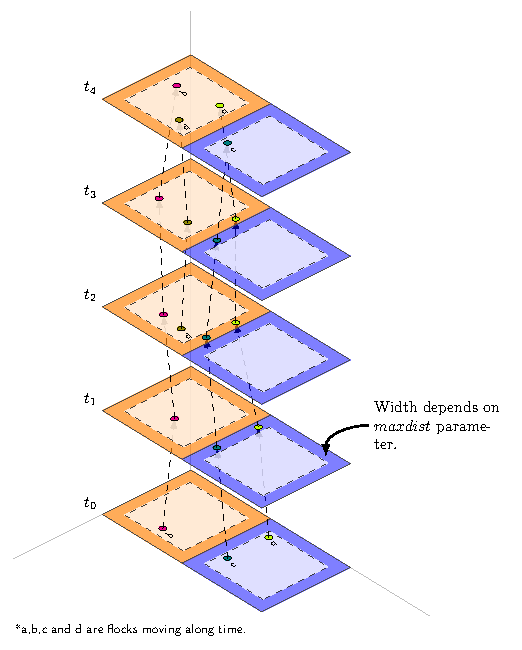
\includegraphics[height=0.9\textheight]
    {chapterPFlocks/figures/plots/11_temporal_partitions/TemporalPartitioning.pdf}
    \caption{CPFs cases moving along different partitions over time.}\label{fig:simple_alternative}
\end{figure}

In the post-processing stage, we evaluate four alternatives for collecting and checking crossing partial flocks (CPFs). The simplest approach is to gather all CPFs and process them sequentially on a single node (the master node). However, due to the large number of partitions and the \textit{maxdist} parameter, the volume of CPFs requiring post-processing can become substantial, leading to a bottleneck that negatively impacts overall performance.

We also evaluate an intermediate approach where the CPFs from a given partition are sent to a middle-level node for processing, based on the quadtree structure used to create the partitions. The choice of which middle-level node to send the CPFs to is determined by a user-defined parameter called \textit{step}. A value of $step = 1$ corresponds to sending CPFs to the immediate parent, $step = 2$ to the grandparent, and so on, until the root is reached. For example, with \textit{step=1}, all CPFs from a partition are first sent to its parent node in the quadtree. The parent node processes its CPFs, but some flocks may still cross outside the parent's safe area.  These leftover CPFs are then passed to the next parent (since $step = 1$), and this process continues until all CPFs are processed, potentially reaching the root node. This approach allows for parallelism in post-processing, as moving to a parent node increases the partition's area and improves the likelihood that CPFs can be resolved at that level. In the experimental section, we test different values of the \textit{step} parameter, such as $step=2$, where CPFs are sent to the grandparent at each stage.  Figure \ref{fig:master-bylevel_alternative} illustrates the Master and By-Level alternatives.

\begin{figure}
    \centering
    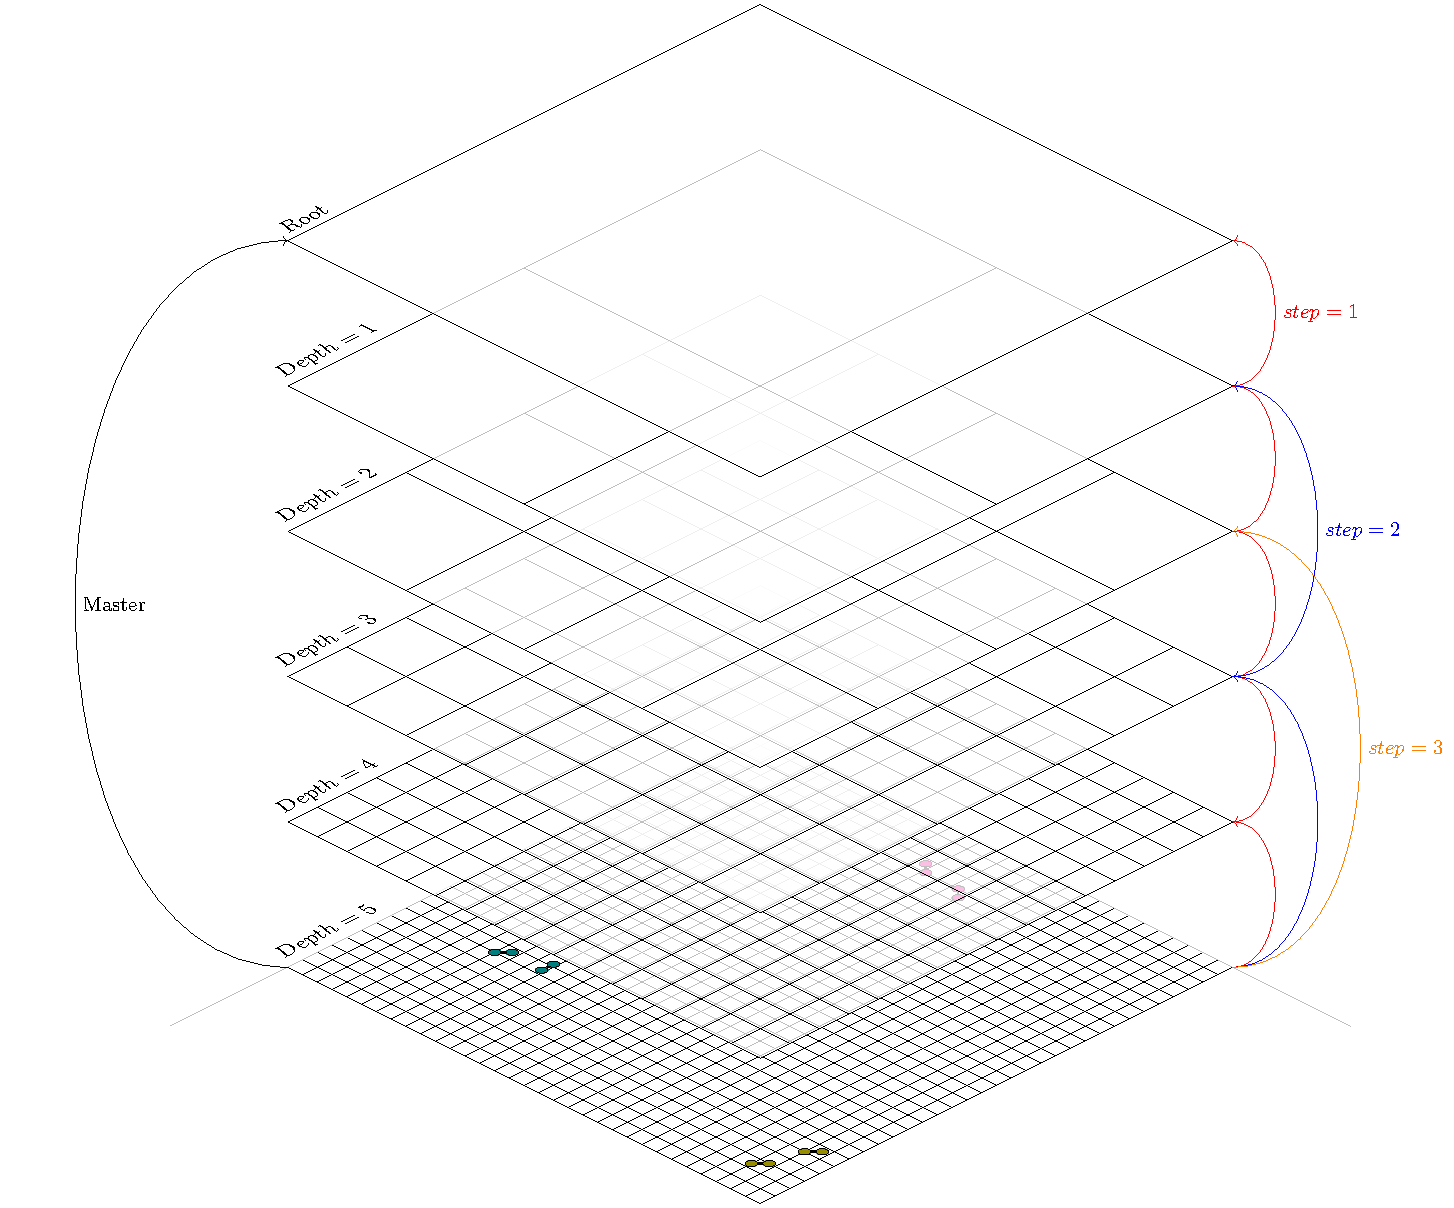
\includegraphics[width=0.75\linewidth]
    {chapterPFlocks/figures/plots/11_temporal_partitions/MasterByLevel}
    \caption{Master and By-Level alternatives.  Different values of $steps$ are illustrated for the By-Level apprach,}\label{fig:master-bylevel_alternative}
\end{figure}

Unlike the previous two approaches, which assign all CPFs from a given partition in the same way (partition-based), the third alternative assigns each CPF individually (CPF-based). For a given CPF $f$, we extend its most recent disk by a ring with a size of \textit{maxdist}, identifying all overlapping partitions for this extended disk —essentially determining which neighboring partitions the objects in $f$ could move to in the next time instant. For each overlapping partition, we retrieve the Least Common Ancestor (LCA) between that partition and $f$'s original partition. CPF $f$ is then sent to the node(s) corresponding to these LCAs. The benefit of this approach is that the LCA can efficiently complete the processing for $f$, as it exploits proximity using \textit{mindist} (see Figure \ref{fig:lca_alternative}).  However, the downside is the increased copying overhead, as $f$ may need to be sent to multiple nodes.

\begin{figure}
    \centering
    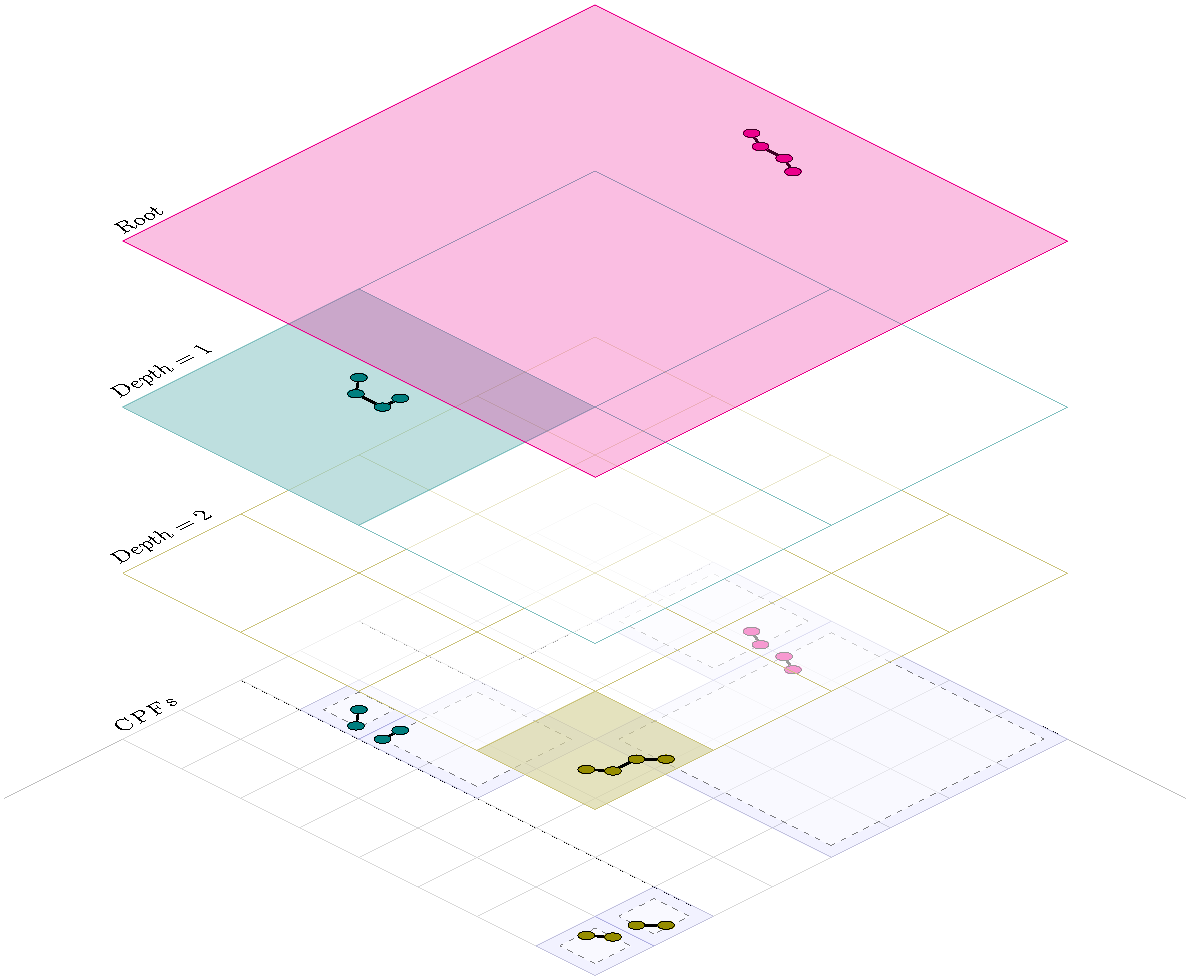
\includegraphics[width=0.75\linewidth]
    {chapterPFlocks/figures/plots/11_temporal_partitions/LCA}
    \caption{LCA alternative and how it resolves CPFs at the nearest shared ancestor of the involved partial flocks.}\label{fig:lca_alternative}
\end{figure}

A limitation of the previous alternatives is that each spatial partition is processed by a single node, which incrementally evaluates all time instances for that partition. The fourth alternative introduces fixed divisions in the temporal domain, based on a user-defined parameter (number of divisions), as illustrated in Figure \ref{fig:cube_alternative}. In this approach, the spatio-temporal space is divided into temporal `cubes,' each of which can be processed by different nodes. For simplicity, we assume that each division spans the same length of time. However, an additional validation step is required to ensure continuity of flocks across temporal divisions.

\begin{figure}
    \centering
    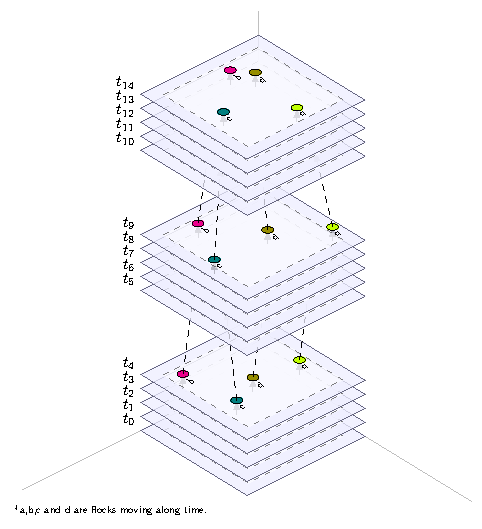
\includegraphics[width=0.9\linewidth]
    {chapterPFlocks/figures/plots/11_temporal_partitions/Cube-based}
    \caption{An alternative division on the time dimension to partition the data into cubes.}\label{fig:cube_alternative}
\end{figure}

\section{Experimental Evaluation}
\subsection{Experimental Setup}
For our experiments, we utilized a 12-node cluster, each running Linux (kernel version 3.10) and Apache Spark 2.4. Each node was equipped with 8 cores, providing a total of 96 cores across the cluster. Each core operated with an Intel Xeon CPU at 1.70 GHz, and each node had 4 GB of main memory.

To evaluate the different approaches, we generated three synthetic datasets with varying characteristics, as detailed in Table \ref{tab:datasets}. These datasets were created using the SUMO simulator \cite{krajzewicz_recent_2012}, by importing traffic networks of Berlin and Los Angeles from OpenStreetMap \cite{haklay2008openstreetmap}. We configured SUMO for pedestrian traffic and generated datasets of 10K, 25K, and 50K pedestrian trajectories. The total duration of the trajectories was set to 10, 30, and 60 minutes, respectively, with positions of pedestrians recorded at one-minute intervals.

\begin{table}
    \centering
    \caption{Description of datasets.}\label{tab:datasets}
    \begin{tabular}{cccc}
        \hline
        Dataset & Number of Trajectories & Total number of points & Maximum Duration (min) \\
        \hline
         Berlin10K &  10000 & 97526 & 10\\ 
         LA25K &  25000 & 1495637 & 30\\
         LA50K &  50000 & 2993517 & 60\\
         \hline
    \end{tabular}
\end{table}

For the partitioning phase, we employed a quadtree structure, though other indexing methods could also be used. The advantage of using a quadtree is its ability to create nodes that tend to have a similar number of objects. The input to this phase is a set of points in the format \textit{(traj-id, x, y, t)}. To construct the quadtree, we begin by sampling 1\% of the input data and inserting this subset into an initially empty quadtree.

A key parameter for the quadtree is the node capacity, denoted as $c$. When the number of points in a node exceeds this capacity, the node splits. After all the sampled points are inserted, we use the Minimum Bounding Rectangles (MBRs) of the leaf nodes as the partitions for our approach. The remaining points are then inserted into these fixed partitions, with no further splits occurring. Each partition is assigned to a different cluster node, where a sequential version of either BFE or PSI is executed locally on the points within that partition.

\subsection{Optimizing the number of partitions for Phase 1.}
The capacity parameter $c$ directly influences the number of partitions in the quadtree. A smaller value of $c$ results in a higher number of partitions, which leads to many smaller tasks that can be distributed across the cluster. However, this can increase the overhead associated with data transmission and, potentially, replication, which may become a bottleneck. Conversely, a larger value of $c$ reduces the number of partitions, resulting in fewer but larger tasks. This increases the workload of the sequential algorithm within each partition, potentially extending the response time for individual jobs.

Figure \ref{fig:optimal_performance} presents the execution time (in seconds) for computing maximal disks (Phase 1) at a specific time instant, using different values of $c$ and $\varepsilon$. The experiments were conducted using the LA25K dataset.
For the case where $\varepsilon = 20m$, we observe that there is an optimal value of $c$ that minimizes the execution time for finding maximal disks, which occurs at $c = 100$ (corresponding to approximately 1300 partitions). Additionally, the optimal value of $c$ varies based on the value of $\varepsilon$. For instance, with a smaller $\varepsilon = 2m$, the execution time is minimized at a larger capacity $c = 500$ (around 250 partitions).
When $\varepsilon$ is large, more pairs of points need to be processed, resulting in a higher number of maximal disks to compute. In such cases, using a smaller value of $c$ creates more partitions within the same spatial area, thereby distributing the workload more evenly across partitions and reducing the amount of work per partition.

\begin{figure}
    \centering
    \begin{tabular}{c c}
         \includegraphics[width=0.45\linewidth]{chapterPFlocks/figures/plots/01_optimal_performance/pflockE2_by_capacity.pdf} & 
         \includegraphics[width=0.45\linewidth]{chapterPFlocks/figures/plots/01_optimal_performance/pflockE5_by_capacity.pdf} \\
         \includegraphics[width=0.45\linewidth]{chapterPFlocks/figures/plots/01_optimal_performance/pflockE10_by_capacity.pdf} &
         \includegraphics[width=0.45\linewidth]{chapterPFlocks/figures/plots/01_optimal_performance/pflockE15_by_capacity.pdf} \\ 
         \includegraphics[width=0.45\linewidth]{chapterPFlocks/figures/plots/01_optimal_performance/pflockE20_by_capacity.pdf} & \\
    \end{tabular}
    \caption{Execution time testing different values for Capacity ($c$) and Epsilon  ($\varepsilon$).}\label{fig:optimal_performance}
\end{figure}

After determining the optimal value of $c$ for a given $\varepsilon$, we further analyzed the behavior of BFE and PSI on the most `demanding' partitions, those 
that required the longest time to complete Phase 1. Since the partitions are processed in parallel across different cores, these demanding partitions have the 
greatest impact on the overall performance. By focusing on these partitions, we can better understand potential bottlenecks and further optimize the system's 
efficiency.

\subsection{Analyzing most costly partitions.}
We began by identifying the top 10 partitions that required the most time to execute the BFE algorithm with $\varepsilon = 20$ meters. For these specific 
partitions, we ran both BFE and PSI while varying $\varepsilon$ from 10 to 20 meters. The Phase 1 execution times are shown in Figure 
\ref{fig:top_time_partitions}, where it is evident that PSI consistently outperformed BFE across all values of $\varepsilon$.

\begin{figure}
    \centering
    \includegraphics[width=\linewidth]{chapterPFlocks/figures/plots/03_top_time_partitions/top_time_partitions.pdf}
    \caption{Comparing the performance of PSI and BFE for time consuming  partitions.} \label{fig:top_time_partitions}
\end{figure}

We further investigated the reasons behind some partitions taking longer to compute. Figure \ref{fig:pairs_performance} shows the Phase 1 execution times per 
partition while varying $\varepsilon$ from 10m to 20m, with partitions ordered by the number of pairs they contain. One key observation is that as $\varepsilon$ 
increases, the number of pairs also increases, since a larger $\varepsilon$ allows for more maximal disks. For instance, with $\varepsilon = 10m$, the maximum 
number of pairs in a partition is around 1800, whereas for $\varepsilon = 20m$, some partitions contain nearly 4000 pairs.

\begin{figure}
    \centering
    \includegraphics[width=0.85\linewidth]{chapterPFlocks/figures/plots/04_pairs_performance/pairs_performance.pdf}
    \caption{Execution time for pairs/disks finding in the dense partition.}
    \label{fig:pairs_performance}
\end{figure}

Another notable observation is that BFE is more sensitive to the density of pairs within a partition than PSI, a difference that becomes more pronounced at 
higher values of $\varepsilon$ (e.g., 18m or 20m). As mentioned earlier, the flexible bounding boxes used by PSI (illustrated in Figure \ref{fig:square}) more 
effectively isolate the relevant points for computing pairs, whereas BFE relies on a fixed grid cell, which makes it less efficient in denser partitions.

A final observation is that a few partitions take significantly more time than others, particularly those with a higher density of pairs. This is directly 
related to the number of maximal disks that need to be computed and subsequently pruned. For example, the partition that takes the longest time when 
$\varepsilon = 20m$ is the one with the highest number of pairs, which corresponds to partition 187 in Figure \ref{fig:top_time_partitions}.

We further analyzed how Phase 1 processing is distributed within the most demanding partition. Figure \ref{fig:dense_stages}.a (for BFE) and Figure 
\ref{fig:dense_stages}.b (for PSI) display the time taken by each Phase 1 stage (refer to Figure \ref{fig:MF_stages}) for partition 187. The most 
resource-intensive stage in both cases is the final step of filtering the disks, where disks whose points are contained within others are removed—this stage 
identifies the \textit{maximal} disks (labeled as `Maximals' in the figure).

This stage is particularly costly because both BFE and PSI must scan a large set of candidate disks, identifying and removing those that are redundant. As 
$\varepsilon$ increases, this processing becomes even more time-consuming, as the number of pairs and candidate disks grows along with $\varepsilon$.

\begin{figure}
    \centering
    \includegraphics[width=\linewidth]{chapterPFlocks/figures/plots/09_dense_stages/dense.pdf} 
    \caption{Processing time for the stages of Phase 1, in (a) standard BFE and (b) standard  PSI.}\label{fig:dense_stages}
\end{figure}

\subsection{Can we reduce pruning time?}
Dense areas pose challenges for pruning, as they are highly sensitive to increases in the value of $\varepsilon$, leading to an exponential growth in the number 
of pairs. To address this, we explored alternative strategies that could enable more effective grouping of points. It is important to note that density-based 
spatial clustering methods, such as DBSCAN \cite{dbscan}, are not suitable for this problem. In very dense regions, these approaches often produce a single 
large cluster, which does not resolve the issue. Additionally, clustering algorithms do not enforce the strict relationships required for a flock, where all 
points must be within a distance of $\varepsilon$ from each other.

Instead, we explored graph-oriented clustering, focusing on the concept of \textit{maximal cliques}. In an undirected graph, a maximal clique is a subset of 
vertices where each vertex is directly connected to every other vertex in the subset. Additionally, the clique is maximal in the sense that it cannot be 
extended by adding more vertices \cite{tomita_clique_2013, bron_algorithm_1973}.

In this context, the points within a partition can be treated as the vertices of an undirected graph, where edges are created between pairs of points that are 
within a distance of $\varepsilon$. By finding the set of maximal cliques in this graph, we identify subsets of points where each point is connected to all 
others in the subset. This means that all points in the clique are at most $\varepsilon$ apart, and no additional points can be added to the subset.
However, not every maximal clique qualifies as a maximal disk. A maximal clique becomes a maximal disk only if it contains at least $\mu$ points and can be 
enclosed by a disk with a radius of $\frac{\varepsilon}{2}$.

To verify whether a maximal clique qualifies as a maximal disk, we introduce the concept of the \textit{Minimum Bounding Circle} (MBC) \cite{welzl_mbc_1991}. 
Given a set of points in Euclidean space, the MBC is the smallest circle that can enclose all the points. For each maximal clique identified within a partition, 
we can quickly check if all points in the clique fit within an MBC with a diameter of $\varepsilon$. If they do, we can immediately report the set of points and 
their MBC as a maximal disk.  However, cliques that do not satisfy this condition must be evaluated using the traditional method. This involves computing the 
potential disk centers, identifying candidate disks, and pruning them, as outlined in Figure \ref{fig:MF_flowchart}. Figure \ref{app:cmbc_flowchar} illustrates the steps described above.

To evaluate the cliques that do not meet the above condition, we implemented two variants. The first variant, termed \textit{COLLECT}, gathers the points from 
all cliques that are not reported as maximal disks, removes duplicates (since points may appear in multiple cliques), and then applies the traditional pruning 
method to the entire set. In the second variant, \textit{EACH}, we apply the pruning procedure independently for each clique that does not qualify as a maximal 
disk.

Figure \ref{fig:cmbc_variants} compares the performance of these variants against the time taken by BFE (a) and PSI (b) for the same stage. Surprisingly, 
neither variant improves execution time. A closer examination reveals that while identifying the cliques and their MBCs is relatively fast, few cliques actually 
qualify as maximal disks. As a result, the overhead involved in processing the remaining cliques is significant, making the original approach more efficient for 
both BFE and PSI.

\begin{figure}
    \centering
    \includegraphics[width=\linewidth] {chapterPFlocks/figures/plots/10_cmbc/cmbc2.pdf}
    \caption{Execution time of the Cliques approach compared to (a) standard BFE and (b) standard PSI.}\label{fig:cmbc_variants}
\end{figure}

\subsection{Relative performance of BFE and PSI Phase 1 using synthetic datasets.}
To further examine the relative performance of the scalable BFE and PSI approaches for Phase 1, we also conducted experiments using a synthetic dataset where we 
could control the values of $c$, $\varepsilon$, and point density. We used a fixed square area of 1000m x 1000m, within which we uniformly distributed 25K, 50K, 
75K, and 100K points.

We experimented with different quadtree capacities ($c$ values of 100, 200, and 300), which resulted in varying numbers of partitions (as shown in Table 
\ref{tab:uniform_ncells}). Both BFE and PSI were tested for phase 1, where maximal disks are identified, using $\varepsilon$ values ranging from 1m to 5m. The 
results are presented in Figure \ref{fig:uniform_performance}.

Overall, PSI demonstrated better performance than BFE, though there were cases (particularly with smaller $\varepsilon$ values) where BFE outperformed PSI. In 
these cases, the smaller $\varepsilon$ generates fewer pairs, and the additional ordering step required by PSI becomes an overhead. However, in the subsequent 
experiments focusing on temporal joins (phase 2, flock creation), we concentrate on the scalable performance of PSI.

\begin{table}
    \centering
    \caption{Number of partitions by capacity and number of points in synthetic uniform datasets.}
    \label{tab:uniform_ncells}
    \begin{tabular}{c|cccc}
              & 25K & 50K  & 75K  & 100K \\
        \hline
        c=100 & 544 & 1024 & 1024 & 2185 \\
        c=200 & 256 & 514  & 1024 & 1024 \\
        c=300 & 256 & 514  & 481  & 1024 \\
    \end{tabular}
\end{table}

\begin{figure}
    \centering
    \includegraphics[width=\linewidth]{chapterPFlocks/figures/plots/05_uniform_performance/uniform_performance.pdf}
    \caption{Performance in an uniform dataset analysing density and capacity with diverse values for epsilon.}\label{fig:uniform_performance}
\end{figure}

\subsection{Evaluation of Phase 2: Temporal join.}
Phase 2 focuses on joining maximal disks across time instants to form flocks. In Section \ref{sec:temporal_join}, we discussed four alternatives: Master, 
By-Level, LCA, and Cube-based. For these experiments, we used the scalable PSI approach due to its robust performance.
First, we compared the Master and By-Level alternatives while varying $\varepsilon$ from 20m to 40m using the Berlin10K dataset (see Figure 
\ref{fig:step_performance}). For the By-Level approach, we tested different step values ranging from 1 to 6. The Master approach proved to be the slowest, due 
to the overhead of sending all CPFs to the root node. The performance of the By-Level approach depends on the step size. A smaller step value (e.g., step 1) 
introduces overhead because CPFs may need to be evaluated at more intermediate nodes before completion. On the other hand, a larger step value reduces 
parallelism by sending more CPFs to intermediate nodes. Based on these experiments, we determined that Step=3 offers the best balance.

We also evaluated the optimal value for the \textit{interval} parameter in the Cube-based approach. Using the LA25K dataset with $\varepsilon=30m$, we tested 
various interval values, ranging from 2 to 12 time instants. This dataset contains 30 time instants in total. The results, shown in Figure 
\ref{fig:interval_performance}, illustrate the trade-offs involved. Lower interval values result in higher parallelism, as more cubes can be processed 
independently. However, this also increases the number of cube crossings for CPFs that need to be checked, which adds to the execution time. Conversely, larger 
interval values reduce parallelism but also decrease the number of CPF crossings. Based on these findings, we selected $interval=6$ as the optimal value for the 
Cube-based approach.

\begin{figure}
    \centering
    \includegraphics[width=0.8\linewidth]{chapterPFlocks/figures/plots/06_step_performance/step_performance.pdf}
    \caption{Root and step alternative for temporal join using the Berlin dataset.}\label{fig:step_performance}
\end{figure}

\begin{figure}
    \centering
    \includegraphics[width=0.8\linewidth]{chapterPFlocks/figures/plots/07_interval_performance/interval-performance.pdf}
    \caption{Interval optimization for the Cube-based alternative for temporal join using the LA25K dataset.}\label{fig:interval_performance}
\end{figure}

Finally, we compared the optimized versions of the By-Level and Cube-based approaches with the Master and LCA methods. Figure \ref{fig:la25k_e_bfe_psi} shows 
the results, including the sequential PSI algorithm as a reference. This experiment was conducted using the LA25K dataset with $\varepsilon$ values ranging from 
5m to 30m. Clearly, all parallel approaches offer significant improvements over the sequential PSI.

To further analyze the relative performance of the scalable approaches, Figure \ref{fig:la25k_e} focuses on the parallel algorithms for the same experiment. 
Interestingly, for very small $\varepsilon$ values, the Master approach performs best —primarily because the limited number of flocks makes sending the CPFs to 
a single node fast and efficient. However, as $\varepsilon$ increases, the Cube-based approach becomes the most effective, leveraging greater parallelism. 
By-Level also improves over the Master approach as $\varepsilon$ grows, as explained in Figure \ref{fig:step_performance}. Similarly, for larger $\varepsilon$ 
values, the LCA approach outperforms By-Level because it more quickly identifies the node that can complete the CPF operations.

We repeated the same experiment with the LA50K dataset, varying $\varepsilon$ from 4m to 20m. The results, shown in Figure \ref{fig:la50k_e}, once again 
demonstrate that the Cube-based approach offers the best performance as $\varepsilon$ increases.

\begin{figure}
    \centering
    \includegraphics[width=0.75\linewidth]{chapterPFlocks/figures/plots/08_sequential_parallel/la25k_e_bfe_psi.pdf}
    \caption{Performance comparing parallel and sequential alternatives in the LA25K dataset.}\label{fig:la25k_e_bfe_psi}
\end{figure}

\begin{figure}
    \centering
    \includegraphics[width=0.75\linewidth]{chapterPFlocks/figures/plots/08_sequential_parallel/la25k_e.pdf}
    \caption{Performance of the 4 parallel alternatives in the LA25K dataset.}\label{fig:la25k_e}
\end{figure}

\begin{figure}
    \centering
    \includegraphics[width=0.75\linewidth]{chapterPFlocks/figures/plots/08_sequential_parallel/la50k_e.pdf}
    \caption{Performance of the 4 parallel alternatives in the LA50K dataset.}\label{fig:la50k_e}
\end{figure}

%\section{Conclusions} \label{sec:conclusions}
We present a novel, scalable approach to discovering moving flock patterns in large trajectory databases. By leveraging distributed frameworks, the proposed method overcomes the limitations of sequential algorithms that struggle with large-scale spatio-temporal datasets. Through partitioning and replication, as well as improvements in pruning and temporal joins, this approach efficiently handles dense data, offering significant performance improvements over traditional methods. The evaluation results demonstrate the scalability and effectiveness of the approach, making it a valuable contribution for analyzing complex movement patterns.

\chapter{Conclusions}
We introduced SDCEL, a scalable approach to compute the overlay operation among two layers that represent polygons from a planar subdivision of a surface. Both 
input layers use the DCEL edge-list data structure to store their polygons. Existing sequential DCEL overlay implementations fail for large datasets. We first 
presented a partition strategy which guarantees that each partition collects the required data from each layer to work independently. 
We also proposed several optimizations to improve performance. Our experimental evaluation using real datasets shows that SDCEL has very good scale-up and 
speed-up performance and can compute the overlay over very large layers (up to 37M edges) in few seconds.


\clearpage
\appendix

\renewcommand\appendixname{}
\renewcommand\appendixpagename{}
\renewcommand{\thechapter}{}
\renewcommand{\thesection}{\Alph{section}}

\chapter{Appendix}
\section{Center computation.}
{\ssp
\begin{algorithm}[h!]
    \caption{Find the centers of given radius which circumference laid on the two input points.}
    \begin{algorithmic}[1]
        \Require Radius $\frac{\varepsilon}{2}$ and points $p_1$ and $p_2$.
        \Ensure Centers $c_1$ and $c_2$.
        
        \Function{FindCenters}{$p_1$, $p_2$, $\frac{\varepsilon}{2}$}
        \State $r^2 \gets (\frac{\varepsilon}{2})^2$
        \State $X \gets p_1.x - p_2.x$
        \State $Y \gets p_1.y - p_2.y$
        \State $d^2 \gets X^2 + Y^2$
        \State $R \gets \sqrt{\lvert 4 \times \frac{r^2}{d^2} - 1 \rvert}$
        \State $c_1.x \gets X + \frac{Y \times R}{2} + p_2.x$
        \State $c_1.y \gets Y - \frac{X \times R}{2} + p_2.y$
        \State $c_2.x \gets X - \frac{Y \times R}{2} + p_2.x$
        \State $c_2.y \gets Y + \frac{X \times R}{2} + p_2.y$
        
        \State \Return $c_1$ and $c_2$
        \EndFunction
    \end{algorithmic}
    \label{app:centers}
\end{algorithm}
}

\clearpage
\section{Disk pruning.}
{\ssp
\begin{algorithm}[h!]
    \caption{Prune disks which are duplicate or subset of others.}
     \begin{algorithmic}[1]
         \Require Set of disks $D$.
         \Ensure Set of disks $D^{\prime}$ without duplicate or subsets.
         
         \Function{PruneDisks}{$D$}
         \State $E \gets \varnothing$
         \ForAll{disk $d_i$ in $D$}
             \State $N \gets d_i \cap D$
             \ForAll{disk $n_j$ in $N$}
                 \If{$d_i$ contains all the elements of $n_j$}
                         \State $E \gets E \cup {n_j}$
                 \EndIf
             \EndFor
         \EndFor        
         \State $D^{\prime} \gets D \setminus E$
         \State \Return $D^{\prime}$
         \EndFunction
     \end{algorithmic}
    \label{app:disks}
\end{algorithm}
}

\clearpage
\section{Clique and MBC approach.}\label{app:cmbc_flowchar}
\renewcommand{\thefigure}{C.1}
\begin{figure}[h!]
    \centering
    \includegraphics[width=0.65\linewidth]{chapterPFlocks/figures/plots/10_cmbc_variants/CMBC_flowchart2.pdf}
    \caption{Schematic description of the Clique and MBC approach.}
\end{figure}



%\nocite{*}
\clearpage
\phantomsection
\bibliographystyle{plain}
\bibliography{thesis}

\end{document}
